\documentclass[notitlepage]{dochead}
\usepackage{psfig}
\usepackage{makeidx}
\usepackage{fancyvrb}
\usepackage{graphicx}

%% Settings for typesetting text as it will be in the book
\setlength{\textheight}{45pc}
\setlength{\textwidth}{34pc}
\setlength{\topmargin}{0in}
\setlength{\oddsidemargin}{-0.25in}
\setlength{\evensidemargin}{\oddsidemargin}

%% Settings for typesetting text for 8.5x11
%\setlength{\textheight}{9.25in}
%\setlength{\textwidth}{6.75in}
%\setlength{\topmargin}{0in}
%\setlength{\oddsidemargin}{-0.25in}
%\setlength{\evensidemargin}{\oddsidemargin}

\setcounter{topnumber}{5}
\setcounter{bottomnumber}{5}
\setcounter{totalnumber}{5}
\renewcommand{\topfraction}{.98}
\renewcommand{\bottomfraction}{.98}
\renewcommand{\textfraction}{0.01}

\raggedbottom

% Shortcut for \noindent
%\newcommand{\noind}{\noindent}

% Macro to introduce invisible (play) character as formatting trick
%\newcommand{\pc}{\mbox{}}

% Macro to define appearance of program source code file name in text
\newcommand{\codename}[1]{\texttt{#1}}

% Macro to define appearance of a term to define
\newcommand{\defn}[1]{\index{#1}\emph{#1}}

% Macro to input code from a source file and label
%
% 1 - Label of code segment
% 2 - source file
%
% Example:  \jcode{Bob}{bob.c}
%
% Bob
% ____________________________________________________________
% #include <stdio.h>...
% \newcommand{\jcode}[2]{\label{#2}\vspace*{0.05in}\hspace*{\fill}{\bf \codename{#1}} \\
% \hrule \small{\listinginput{0}{#2}} \hrulefill\\ \hspace*{\fill}{\bf \codename{#1}}}
% I hope none of our programs are over 10000 lines long!
% 1 - Last line number from file (optional) - SPECIFY IN [] when using
% 2 - Title of code segment
% 3 - source file
% 4 - First line number to display
% 5 - First line number from file (start from 1)
%
% Example:  \jcode{Bob}{bob.c}{0}{1}
%           \jcode[20]{Bob}{bob.c}{0}{1}
\renewcommand{\theFancyVerbLine}{\arabic{FancyVerbLine}}
% 1 - Title of code segment
% 2 - source file
\newcommand{\jcodestartdivide}[2]{\index{#2}\label{#2}\vspace*{0.05in}\hspace*{\fill}\textbf{\codename{#1}} \\ \hrule}
% 1 - Title of code segment
\newcommand{\jcodestopdivide}[1]{\hrulefill \\ \hspace*{\fill}\textbf{\codename{#1}}}
% 1 - Last line number from file (optional) - SPECIFY IN [] when using
% 2 - source file
% 3 - First line number to display
% 4 - First line number from file (start from 1)
%\newcommand{\jcodenoem}[4][10000]{\VerbatimInput[numbers=left,fontfamily=courier,fontsize=\small,firstnumber=#3,
\newcommand{\jcodenoem}[4][10000]{\VerbatimInput[numbers=left,fontfamily=courier,fontsize=\normalsize,firstnumber=#3,
firstline=#4,lastline=#1,xleftmargin=0.23in,numbersep=5pt]{#2}}
% 1 - Last line number from file (optional) - SPECIFY IN [] when using
% 2 - source file
% 3 - First line number to display
% 4 - First line number from file (start from 1)
\newcommand{\jcodeem}[4][10000]{\VerbatimInput[numbers=left,fontfamily=courier,fontsize=\normalsize,firstnumber=#3,
firstline=#4,lastline=#1,xleftmargin=0.23in,numbersep=5pt,fontseries=b]{#2}}
\newcommand{\jcode}[5][10000]{\jcodestartdivide{#2}{#3} \jcodenoem[#1]{#3}{#4}{#5} \jcodestopdivide{#2}}

% Use this to connect previous code snippets
%
% Example:  This prints the start divider, the first 5 lines normally, the remaining lines emphasized (bold)
%           and the stop divider
% \jcodestartdivide{Bob}{bob.c}
% \jcodenoem[5]{bob.c}{0}{1}
% \jcodeconnect
% \jcodeem{bob.c}{0}{6}
% \jcodestopdivide{Bob}
\newcommand{\jcodeconnect}{\vspace*{-0.27in}}

\newcommand{\jtitle}{JUNK}
\newcommand{\jfile}{JUNK}

% Macro to create pamphelet part.  Pamphlet consist of (in decreasing 
% order of importance): Parts, chapters (\pampchap), sections
% (\pampsect), and subsection (\pampsubsect, \apihdr)
%
% 1 - Part name (e.g. Tutorial)
%
% Example:  \pamppart{Tutorial}
%
% <new page>
% ...
%                    Part I:
% ...
%                   Tutorial
% ...
% \newcounter{partcnt}
% \renewcommand{\thepartcnt}{\Roman{partcnt}}
% \newcommand{\pamppart}[1]{
% \stepcounter{partcnt}
% \newpage % create new page
% \thispagestyle{empty}  % No page number

% \vspace*{\fill}

% \begin{center}  % Include pamphlet part major name on one line 
%                 % and minor name on next line
% {\bf\Huge Part \thepartcnt\\ \vskip .5in #1}
% \addtocontents{toc}{\vspace*{0.1in}\noindent{\LARGE\bf Part \Roman{partcnt}\hfill #1}\vspace*{0.1in}}
% \end{center}
% \vfill  % Fill remainder of page

% \newpage  % create new page
% }

\newcommand{\pamppart}[1]{\part{#1}}

% Macro to create chapter header (e.g. Introduction)
%
% 1 - Chapter name
%
% Example: \pampchap{Introduction}
%
% 1 Introduction (right justified)
%
% \newcounter{chapcnt} %[partcnt] Add back in to get chapcnt to restart with each part
% \renewcommand{\thechapcnt}{\arabic{chapcnt}}
% \newcommand{\pampchap}[1]{\stepcounter{chapcnt}\label{chap:#1}\vspace*{0.1in}\noindent{\Large\bf Chapter~\thechapcnt:  #1}\\[0.1in]\addcontentsline{toc}{section}{\thechapcnt~#1}}

%\newcommand{\pampchap}[1]{\newpage%
%\stepcounter{chapter}\vspace*{0.1in}\noindent{\LARGE\bf Chapter~\thechapter:  #1}
%\\[0.1in]\addcontentsline{toc}{chapter}{\protect\numberline{\thechapter}#1}}

\newcommand{\pampchap}[1]{\chapter{#1}}

% Macro to create section header (e.g. What is a socket)
%
% 1 - Section name
%
% Example: \pampsect{What is a socket}
%
% 1.1 What is a socket
% ___________________________________________________________
%
% \newcounter{sectcnt}[chapcnt]
% \renewcommand{\thesectcnt}{\arabic{chapcnt}.\arabic{sectcnt}}
% \newcommand{\pampsect}[1]{\stepcounter{sectcnt}\vspace*{0.1in}\noindent{\bf \thesectcnt~#1} \hrulefill\addcontentsline{toc}{subsection}{\thesectcnt~#1}}

\newcommand{\pampsect}[1]{\section{#1}}

% Macro to create subsection header (e.g. What is a socket)
%
% 1 - Subsection name
%
% Example: \pampsubsect{What is a socket}
%
% 1.1.1 What is a socket
%
% \newcounter{subsectcnt}[sectcnt]
% \renewcommand{\thesubsectcnt}{\arabic{chapcnt}.\arabic{sectcnt}.\arabic{subsectcnt}}
% \newcommand{\pampsubsect}[1]{\stepcounter{subsectcnt}\vspace*{0.1in}\noindent{\bf \thesubsectcnt~#1}\addcontentsline{toc}{subsection}{\thesubsectcnt~#1}}

\newcommand{\pampsubsect}[1]{\subsection{#1}}

% Macro to create header for an API chapter (e.g. Socket Creation)
%
% 1 - API chapter name
%
% Example: \apichap{Socket Creation}
%
%\newcommand{\apichap}[1]{\pagebreak[4]\label{api:#1}\vspace*{0.1in}%
\newcommand{\apichap}[1]{\vspace*{0.1in}%
\noindent{\Large\bf #1}\\[0.1in]\addcontentsline{toc}{chapter}{#1}}

% Macro to create header for API (e.g. socket())
%
% 1 - API function name
% 2 - Additional phrase
%
% Example: \apihdr{listen()}{- Stream/TCP socket only}
%
% o listen() - Stream/TCP socket only
% ----------
%
\newcommand{\apihdr}[2]{\noindent $\circ$ \texttt{\large \underline{#1}#2}%
\addcontentsline{toc}{section}{#1}}

% Macros for appearance of functions (\fnc), function types (\type), and 
% function parameters (\var)
\newcommand{\var}[1]{\textsl{#1}}
\newcommand{\varsys}[1]{\var{#1}\index{#1}}
\newcommand{\const}[1]{\textsc{#1}}
\newcommand{\constsys}[1]{\const{#1}\index{#1}}
\newcommand{\type}[1]{\textbf{#1}}
\newcommand{\typesys}[1]{\type{#1}\index{#1}}
\newcommand{\fcn}[1]{\texttt{#1}}
\newcommand{\fcnsys}[1]{\fcn{#1}\index{#1}}
\newcommand{\structmem}[1]{\texttt{#1}}
\newcommand{\param}[1]{\var{#1}}
\newcommand{\file}[1]{\texttt{#1}}
\newcommand{\fcnref}[1]{\texttt{#1}}
\newcommand{\fcnrefsys}[1]{\fcnref{#1}\index{#1}}
\newcommand{\returncode}[1]{$#1$}
\newcommand{\exec}[1]{\texttt{#1}}
\newcommand{\errnum}[1]{\constsys{#1}}
\newcommand{\errno}{\texttt{errno}}
\newcommand{\codesegref}[1]{\texttt{#1}}

% Macro for code file reference
\newcommand{\coderef}[1]{\file{#1} (pg.~\pageref{#1})}

% Macro for defining a parameter to an API function
\newcommand{\paramdesc}[2]{\var{#1} & --- & #2 \\}

% Macro for adding an include file
\newcommand{\newincl}[1]{\#include $<$#1$>$}

% Macro to place box around API entries to avoid page breaks
\newcommand{\apibox}[1]{\parbox{\textwidth}{#1}}

% Macro to define an API function
% 
% Parameters:
% 1 - function name (e.g. socket())
% 2 - option phrase (e.g. Stream/TCP sockets only)
% 3 - function description (e.g. creates a socket...)
% 4 - include files
% 5 - function declaration (e.g. socket(int ...))
% 6 - parameter table (e.g. \begin{tabular}...)
% 7 - return information (e.g. -1 for failure...)
%
\newcommand{\apifunc}[7]{
\index{#1}
\apihdr{#1}{#2}\\[0.1in]
%\vspace*{0.1in}
#3
\begin{quote}

#4	

#5

\begin{quote}
#6
\end{quote}
#7
\end{quote}
}

% No parameter version of \apifunc
\newcommand{\apifuncnp}[6]{
\index{#1}
\apihdr{#1}{#2}\\[0.1in]
%\vspace*{0.1in}
#3  #6
\begin{quote}

#4	

\fcn{#5}
\end{quote}
}

% Macro for code references in api specifications
%
% 1 - Name of program
% 2 - Program page reference
% 3 - Lines
\newcommand{\seecode}[3]{\noindent See \codename{#1} pg.~\pageref{#2}/ln. #3 \\}

% Top-level code description environment
\newenvironment{topcode}{\begin{enumerate}}{\end{enumerate}}

% Macro for top level code description
%
% Parameters:
% 1 - Tag
% 2 - Line numbers
%
\newcommand{\tlcitem}[2]{\item \textbf{#1:} line {#2}}
\newcommand{\tlcitems}[2]{\item \textbf{#1:} lines {#2}}

% Bottom-level code description environment
\newenvironment{bottomcode}{\begin{itemize}}{\end{itemize}}

% Macro for top level code description
%
% Parameters:
% 1 - Tag
% 2 - Line numbers
%
\newcommand{\blcitem}[2]{\item \textbf{#1:} line {#2}}%
\newcommand{\blcitems}[2]{\item \textbf{#1:} lines {#2}}%
%
% Constant for default client IP/name and server IP/name
\newcommand{\clientIPiv}{169.1.1.2}
\newcommand{\clientName}{tractor.farm.com}
\newcommand{\serverIPiv}{169.1.1.1}
\newcommand{\serverName}{base.farm.com}
\newcommand{\clientIPvi}{FE80::2}
\newcommand{\serverIPvi}{FE80::1}
\newcommand{\mkpweb}{\textit{www.mkp.com}}

% Termination character
\newcommand{\termchar}{0}

% Names for queues. XXXX  CHANGE THESE -- KLC
\newcommand{\sque}{\textit{SendQ}}
\newcommand{\rque}{\textit{RecvQ}}
\newcommand{\dque}{\textit{Delivered}}
\newcommand{\sqsize}{\textit{SQS}}
\newcommand{\rqsize}{\textit{RQS}}

% Environment for including shell execution
%
% Parameters:
% 1 - C
% 2 - Line numbers
%
\newcommand{\prompt}{\% }
\newcommand{\typed}[1]{\textbf{#1}}
\newcommand{\response}[1]{#1}
\newenvironment{shell}
{\begin{quote} \ttfamily \vskip -.1in}
{\end{quote}\vskip -.1in}

% EPS figure insertion
%
% Parameters:
% 1 - Filename
% 2 - Options (e.g. ,width=11in,height=12in)
%
% Example: \jfig{bob.eps}{}
%
\newcommand{\jfig}[2]{\centerline{\psfig{file=#1#2}}} %XXX don't use this!
\newcommand{\jfigs}[2]{\begin{center}\includegraphics[width={#2}]{#1}%
\end{center}}

% Inline code insertion
\DefineVerbatimEnvironment%
  {inlinecode}{Verbatim}
  {fontfamily=courier,fontsize=\normalsize,xleftmargin=.25in}

% Inline function definitions
\newenvironment{inlinefcn}
{\vspace*{0.2in}\noindent\rule{\textwidth}{1pt}\\[0.1in]}
{\\[0.1in]\noindent\rule{\textwidth}{1pt}\vspace*{0.1in}}

% Ken macros
\newcommand{\Fig}[1]{Figure~\ref{#1}}
\newcommand{\Sect}[1]{Section~\ref{#1}}

% List redefinitions
\newcounter{enumct}
\renewenvironment{enumerate}{\begin{list}%
{\arabic{enumct}. }%
{\usecounter{enumct}
\setlength{\parsep}{0.15ex plus0.1ex minus0.1ex}
\setlength{\topsep}{0.15ex plus0.1ex minus0.1ex}
\setlength{\partopsep}{0.15ex plus0.1ex minus0.1ex}
%\setlength{\leftmargin}{0in}
\setlength{\itemsep}{0.15ex plus0.1ex minus0.1ex}}}
{\end{list}}

\renewenvironment{itemize}{\begin{list}%
{$\bullet$}%
{\setlength{\parsep}{0.15ex plus0.1ex minus0.1ex}
\setlength{\topsep}{0.15ex plus0.1ex minus0.1ex}
\setlength{\partopsep}{0.15ex plus0.1ex minus0.1ex}
%\setlength{\leftmargin}{0in}
\setlength{\itemsep}{0.15ex plus0.1ex minus0.1ex}}}
{\end{list}}

\newcommand{\copyrightnotice}{%
\begin{center}
\copyright 2000, Morgan Kaufmann Publishers.  Reproduced with permission from 
\emph{The Pocket Socket Guide in C}
\end{center}}

% Thought question section -- XXXX DEPRECATED
\newenvironment{tquestlist}{\section*{Thought Questions}\begin{enumerate}}{\end{enumerate}}
% Exercises section
\newenvironment{exercises}{\section*{Exercises}\begin{enumerate}}{\end{enumerate}}
% Marginal mark for points to be emphasized
\newsavebox{\NB}
\newcommand{\callout}[1]{\textbf{#1}\marginpar{\usebox{\NB}}}
\sbox{\NB}{\Huge !*!}
  % Get all user-defined commands

%\makeindex

\begin{document}

\newpage \tableofcontents \newpage

\newpage
\thispagestyle{empty}
%\vspace{1in}
\vfill
\begin{center}
{\Huge\textbf{TCP/IP Sockets in C}} \\
{\Large\textbf{Practical Guide for Programmers, Second Edition}  \\[.2in]}
{\bf Michael J. Donahoo \\
Kenneth L. Calvert \\[.2in]}
\end{center}

\section*{Preface to the Second Edition}

When we wrote the first edition of this book, it was not very common
for college courses on networking to include programming components.
That seems difficult to believe now, when the Internet has become so
important to our world, and the pedagogical benefits of hands-on programming
and real-world protocol examples are so widely accepted.
%
Although there are now other languages that provide access
to the Internet, interest in the
original C-based \emph{Berkeley Sockets} remains high.
The Sockets  API (application programming interface) for
networking was developed at UC Berkeley in the 1980's
for the BSD flavor of Unix---one of the very first
examples of what would now be called an ``open source'' project.

The Sockets API and the Internet both grew up in a world of many
competing protocol families---IPX, Appletalk, DECNet, OSI, and SNA in
addition to TCP/IP---and Sockets was designed to support them all.
Fewer protocol families were in common use by the time we wrote the
first edition of this book, and the number today is even smaller.
Nevertheless,  as we predicted in the first edition, the sockets API remains
important for those who want to design and build distributed
applications that use the Internet---i.e., which use TCP/IP.
And the interface has proven robust enough
to support the new version of the Internet Protocol (IPv6), which is
now supported on virtually all common computing platforms.

Two main considerations motivated this second edition.
First, based on our own experience and feedback from others,
we found that some topics needed to be presented in more
depth and that others needed to be expanded.
%
The second consideration is the increasing acceptance and use of IP
version~6, which is now supported by essentially all current end
system platforms.  At this writing, it is not possible to use IPv6 to
exchange messages with a large fraction of hosts on the Internet, but
it \emph{is\/} possible to assign an IPv6 address to many of them.
While it is still too early to tell whether IPv6 will take over the
world, it is not too early to start writing applications to be
prepared.

\subsection*{Changes from the First Edition}

We have updated and considerably expanded most of the material, having
added two chapters.  Major changes from the first edition include:
\begin{itemize}
\item
IP version 6 coverage.  We now include three kinds of code:
IPv4-specific, IPv6-specific, and generic.  The code in the
later chapters is designed to work with either protocol version on
dual-stack machines.
\item
An additional chapter on socket programming in C++
(contributed by David B.\ Sturgill).
% XXXXXXXX CHECK IT
The PracticalSocket library provides wrappers for basic socket functionality.
These allow an instructor to teach socket programming to
students without C programming background by giving them a library and
then gradually peeling back the layers.  Students can start
developing immediately after understanding addresses/ports and
client/server.  Later they can be shown the details of socket programming by
peeking inside the wrapper code.
Those teaching a subject that uses networking (e.g., OS) can
use the library and only selectively peel back the cover.
\item
Enhanced coverage of data representation issues and strategies for
organizing code that sends and receives messages.  In our
instructional experience we find that students have less and less
understanding of how data is actually stored in memory,\footnote{We
speculate that this is due to the widespread use of C++ and Java,
which hide such details from the programmer, 
in undergraduate curricula.} so we have
attempted to compensate with more discussion of this important
issue.  At the same time, internationalization will only increase in
importance, and thus we have included basic coverage of
wide characters and encodings.
\item
Omission of the reference section.  The descriptions of
most of the functions that make up the Sockets API have been collected
into two chapters.  However, with so many on-line sources of reference
information---including ``man pages''---available,
we chose to leave out the complete listing of the API in favor of
more code illustrations.
\item
Highlighting important but subtle facts and caveats.  Typographical devices
call out important concepts and information that might otherwise
be missed on first reading.
\end{itemize}

Although the scope of the book has expanded, we have not included
everything that we might have (or even that we were asked to include);
examples of topics left for more comprehensive texts (or the
next edition): raw sockets and programming with Winsock.

%% Excellent reference books on TCP/IP socket programming
%% exist, but they are too large and comprehensive to be considered as a
%% supplement to a networking text.  UNIX ``man pages'' are great for
%% reference but do not make a very good tutorial.

%% Enabling students to get their hands on real network services via the
%% sockets interface has several benefits.  First, for a surprising
%% number of people, socket programming is the first exposure to concrete
%% realizations of concepts previously seen only in the abstract.
%% Dealing with the very real consequences of messy details, such as the
%% layout of data structures in memory, seems to trigger a kind of
%% epiphany in some students, and this experience has consequences far
%% beyond the networking course.  Second, we find that students who
%% understand how application programs \emph{use} the services of TCP/IP
%% generally have an easier time grasping the principles of the
%% underlying protocols that \emph{implement} those services. Finally,
%% basic socket programming skills are a springboard to more advanced
%% assignments, which support learning about routing algorithms,
%% multimedia protocols, medium access control, and so on.

\subsection*{Intended Audience}

We originally wrote this book so we'd have something to hand our students
when we wanted them to learn socket programming, so we wouldn't have
to take up valuable class time teaching it.  In the years since
the first edition, we have learned a good deal
about the topics that students need lots of help on, and those where
they do not need as much handholding.  We also found that
our book was appreciated at least as much by practitioners who were
looking for a gentle introduction to the subject.
%
Therefore this book is aimed simultaneously at two general audiences:
students in introductory courses in computer networks (graduate or
undergraduate) with a programming component, and
practitioners who want write their own programs that
communicate over the Internet.
For students, it is intended as a supplement, not as a primary text
about networks.
Although this second edition is significantly bigger in size and scope than
the first, we hope the book will still be considered a good value in
that role.
%
For practitioners who just want to write some useful code, it should
serve as a standalone \emph{introduction}---but readers in that
category should be warned that this book will not make them
experts. 
%
Our philosophy of learning by 
doing has not changed, nor has our approach of providing a concise
tutorial sufficient to get one started learning on one's own, and
leaving the comprehensive details to other authors.
For both audiences our goal is to
take you far enough so that you can start experimenting and
learning on your own.

\subsection*{Assumed Background}

We assume basic programming skills and experience with C and UNIX.
You are expected to be conversant with C concepts such as pointers
and type casting, and should have a basic understanding of
the binary representation of data.  Some of our examples are factored
into files that should be compiled separately; we assume that you can deal with
that.

Here is a little test: If you can puzzle out what the following code
fragment does, you should have no problem with the code in this book:

\begin{inlinecode}
  typedef struct {
    int a;
    short s[2];
  } MSG;

  MSG *mp, m = {4, 1, 0};
  char  *fp, *tp;
  mp = (MSG *) malloc(sizeof(MSG));
  for (fp = (char *)m.s, tp = (char *)mp->s; tp < (char *)(mp+1);)
     *tp++ = *fp++;
\end{inlinecode}

If you do not understand this fragment, do not despair (there is
nothing quite so convoluted in our code), but you might want to refer
to your favorite C programming book to find out what is going on here.

You should also be familiar with the UNIX notions of process/address
space, command-line arguments, program termination, and regular file
input and output. The material in Chapters 4 and 5 assumes a somewhat
more advanced grasp of UNIX.  Some prior exposure to networking concepts
such as protocols, addresses, clients, and servers will be helpful.

\subsection*{Platform Requirements and Portability}

Our presentation is UNIX-based.  When we were developing this
book, several people urged us to include code for Windows as well as
UNIX.  It was not possible to do so for various reasons including the
target length (and price) we set for the book.

For those who only have access to Windows platforms, please note that
the examples in the early chapters require minimal modifications to work
with WinSock.  (You have to change the include files and add a setup
call at the beginning of the program and a cleanup call at the end.)
Most of the other examples also require very slight additional
modifications.  However, some are so dependent on the UNIX
programming model that it does not make sense to port them to WinSock.
%
WinSock-ready versions of the other examples, as well as detailed
descriptions of the code modifications required, are available from
the book's Website at \emph{www.mkp.com/socket} [XXX URL].  Note also that
almost all of our example code works with minimal modifications under
the \textbf{Cygwin} Unix library package for Windows, which is
available online.

For this second edition, we have adopted the C99 language standard.
This version of the language is supported by most compilers and offers
so many readability-improving advantages---including line-delimited
comments, fixed-size integer types,
and declarations anywhere in a block---that we could not
justify not using it.

Our code makes use of the ``Basic Socket Interface Extensions for
IPv6''~\cite{RFC3493}.
Among these extensions is a new and different interface to the name system.
Because we rely completely on this new interface
(\fcn{getaddrinfo()}), our generic code may not run on some older
platforms.  However, we expect that most modern systems will run our
code just fine.

The example programs included here have all been tested (and
should compile and run without modification) on both Linux and
MacOS.
% XXXXXXX
Header (\texttt{.h}) file locations and dependencies are, alas, not quite
standard and may require some fiddling on your system. Socket option
support also varies widely across systems; we have tried to focus on
those that are most universally supported.  Consult your API
documentation for system specifics.  (By ``API documentation'' we mean
the ``man pages'' for your system.  To learn about this, type ``man man''.)

Please be aware that although we strive for a basic level of
robustness, the primary goal of our
code examples is pedagogy, and the code is \textbf{not production
quality.}  We have sacrificed some robustness for brevity and clarity,
especially in the generic server code.  (It turns out to be rather
nontrivial to write a server that works under all combinations
of IPv4 and IPv6 protocol configurations and also maximizes the
likelihood of successful client connection under all circumstances.)

\subsection*{This Book Will Not Make You an Expert!}

We hope this
second edition will be useful as a resource, even to those who already
know quite a bit about sockets.
As with the first edition, we learned some things in writing it.
But becoming an expert
takes years of experience, as well as other, more comprehensive
sources~[\cite{ComerV3}, \cite{StevensUNP}]. 

%% The first part of the book is a tutorial, which begins with ``just
%% enough'' of the big picture, then quickly gets into code basics via
%% some example programs.  The first four chapters aim to get you quickly
%% to the point of constructing simple clients and servers, such as might
%% be needed to complete introductory assignments.  After that we branch
%% out in Chapter~5, introducing some of the many different ways to use
%% sockets.  Chapter~6 returns to basic socket operation to provide more
%% in-depth coverage of some of the underlying mechanisms and some
%% pitfalls to watch out for.  Chapter~7 describes domain names and how
%% they can be used to obtain Internet addresses.

The first chapter is intended to give ``just enough'' of the big
picture to get you ready to write code.  Chapter~\ref{chap:tcp}
shows you how to write TCP clients and servers using either IPv4 or IPv6.
Chapter~\ref{chap:addrindep} shows how to make your clients and
servers use the network's name service, and also shows how to make
them IP-version-independent.  Chapter~\ref{chap:udp} covers UDP.
Chapters~\ref{chap:encoding} and~\ref{chap:advanced} provide
background needed to write more programs, while
Chapter~\ref{chap:under} gives relates some of what is going on in the
Sockets implementation to the API calls; these three are essentially
independent and may be presented in any order.
Finally, Chapter~\ref{chap:cpp} presents a C++ class library that
provides simplified access to socket functionality.

Throughout the book, certain statements are highlighted like this:
\callout{This book will not make you an expert!}  Our goal is to bring
to your attention those subtle but important facts and ideas that one
might miss on first reading.  The marks tell you to ``\textbf{note
well} whatever is in bold.


\subsection*{Acknowledgments}

Many people contributed to making this
book a reality.  In addition to all those who helped us with the first
edition (Michel Barbeau, Steve Bernier,
Arian Durresi,
Gary Harkin, Ted Herman,
Lee Hollaar, David Hutchison, Shunge Li, Paul Linton,
Ivan Marsic, Willis Marti,
Kihong Park, Dan Schmitt, Michael Scott,  Robert Strader, 
Ben Wah,
and Ellen Zegura), we especially thank David B.\ Sturgill, who
contributed code and text for Chapter~\ref{chap:cpp}, 
%
Bobby Krupczak for
his help reviewing the draft of this second edition.
Finally, to the folks at Morgan Kaufmann/Elsevier---Rick Adams, our
editor, Maria Alonso, and our production editor [N.N.]---thank you for
your patience, help, and caring about the quality of our book.

\subsection*{Feedback}

We are very interested in weeding out
errors and otherwise
improving future editions/printings, so if you find one, please send
email to either of us.  We will maintain an errata list on the book's
Web page.

\vspace{1.4ex}
\noindent
\textsl{
M.J.D. \texttt{jeff\_donahoo@baylor.edu}\\
K.L.C \texttt{calvert@netlab.uky.edu}
}

%\copyrightnotice


\setcounter{page}{1}

\chapter{Introduction}
\label{chap:intro}

Today people use computers to make phone calls, watch TV, send
instant messages to their friends, play games with other people,
and buy most anything you can think of---from songs to automobiles.  The
ability for programs to communicate over the Internet makes all this
possible.  It's hard to say how many individual computers are now
reachable over the Internet, but we can safely say that it is growing
rapidly; it won't be long before the number is in the billions.
Moreover, new applications are being developed every day.  With the
push for ever increasing bandwidth and access, the impact of the
Internet will continue to grow for the forseeable future.

How \emph{does\/} a program communicate with another program over a
network?  The goal of this book is to \emph{start\/} you on the road
to understanding the answer to that question, in the context of the
C programming language.  For a long time, C was the language of choice
for implementing network communication softward.  Indeed, the 
application programming interface (API) known as \defn{sockets} was
first developed in C.

Before we delve into the details of sockets, however, it is worth
taking a brief look at the big picture of networks and protocols to
see where our code will fit in.  Our goal here is \emph{not\/} to
teach you how networks and TCP/IP work---many fine texts are available
for that purpose~\cite{ComerV1,ComerV3,PandD,StevensV1,StevensV2}---but
rather to introduce some basic concepts and terminology.

\section{Networks, Packets, and Protocols}

A computer network consists of machines interconnected by
communication channels. We call these machines \emph{hosts} and
\emph{routers}.  Hosts are computers that run applications such as
your Web browser, your IM agent, or a file-sharing program.
The application programs running on hosts are the
real ``users'' of the network.  Routers (also called \emph{gateways}) are machines whose job is to
relay, or \emph{forward}, information from one communication channel
to another.  They may run programs but typically do not run
application programs.  For our purposes, a \emph{communication
channel} is a means of conveying sequences of bytes from one host to
another; it may be a wired (e.g., Ethernet), a wireless (e.g., WiFi), or
other connection.

Routers are important simply because it is not practical to connect
every host directly to every other host. Instead, a few hosts connect
to a router, which connects to other routers, and so on to form the
network.  This arrangement lets each machine get by with a relatively
small number of communication channels; most hosts need only one.
Programs that exchange information over the network, however, do not
interact directly with routers and generally remain blissfully unaware
of their existence.

By \emph{information} we mean sequences of {bytes} that are
constructed and interpreted by programs. In the context of computer
networks, these byte sequences are generally called \emph{packets}.  A
packet contains control information that the network uses to do its
job and sometimes also includes user data.  An example is information
identifying the packet's destination. Routers use such control
information to figure out how to forward each packet.

A \emph{protocol} is an agreement about the packets exchanged by
communicating programs and what they mean.  A protocol tells how
packets are structured---for example, where the destination
information is located in the packet and how big it is---as well as
how the information is to be interpreted.  A protocol is usually
designed to solve a specific problem using given capabilities.  For
example, the \emph{HyperText Transfer Protocol (HTTP)} solves the
problem of transferring hypertext objects between servers, where they
are stored or generated,
and Web browsers that make them visible and useful to users.
Instant messaging protocols solve the problem of enabling two or more
users to exchange brief text messages.

Implementing a useful network requires solving a large number of
different problems. To keep things manageable and modular,
different protocols are designed to solve different sets of problems.
TCP/IP is one such collection of solutions, sometimes called a
\emph{protocol suite}.  It happens to be the suite of protocols used
in the Internet, but it can be used in stand-alone private networks as
well.  Henceforth when we talk about the \emph{network}, we mean any
network that uses the TCP/IP protocol suite.  The main protocols in
the TCP/IP suite are the Internet Protocol (IP), the Transmission
Control Protocol (TCP), and the User Datagram Protocol (UDP).

It turns out to be useful to organize protocols into \emph{layers};
TCP/IP and virtually all other protocol suites are organized this way.
Figure~\ref{fig:IPnet} shows the relationships among the protocols,
applications, and the sockets API in the hosts and routers, as well as
the flow of data from one application (using TCP) to another.  The
boxes labeled TCP, UDP, and IP represent implementations of those
protocols. Such implementations typically reside in the operating
system of a host.  Applications access the services provided by UDP
and TCP through the sockets API, represented as a dashed line.  The arrow 
depicts the flow of data
from the application, through the TCP and IP implementations, through
the network, and back up through the IP and TCP implementations at the
other end.

\begin{figure}[htbp]
\jfigs{figures/IPnet.eps}{\textwidth}
\caption{\label{fig:IPnet}A TCP/IP Network}
\end{figure}

In TCP/IP, the bottom layer consists of the underlying communication
channels---for example, Ethernet or dial-up modem connections.  Those
channels are used by the \emph{network layer}, which deals with the
problem of forwarding packets toward their destination (i.e., what
routers do).  The single network layer protocol in the TCP/IP suite is
the Internet Protocol; it solves the problem of making the sequence of
channels and routers between any two hosts look like a single
host-to-host channel.

The Internet Protocol provides a \emph{datagram} service: every packet
is handled and delivered by the network independently, like letters or
parcels sent via the postal system.  To make this work, each IP packet
has to contain the \emph{address} of its destination, just as every
package that you mail is addressed to somebody.  (We'll say more about
addresses shortly.)  Although most delivery companies guarantee
delivery of a package, IP is only a best-effort protocol: it attempts
to deliver each packet, but it can (and occasionally does) lose,
reorder, or duplicate packets in transit through the network.

The layer above IP is called the \emph{transport layer}.  It offers a
choice between two protocols: TCP and UDP.  Each builds on the service
provided by IP, but they do so in different ways to provide different
kinds of transport, which are used by \emph{application protocols}
with different needs.  TCP and UDP have one function in common:
addressing.  Recall that IP delivers packets to hosts; clearly, a
finer granularity of addressing is needed to get a packet to a
particular application program, perhaps one of many using the network on the
same host.  Both TCP and UDP use addresses, called \emph{port
numbers}, to identify applications within hosts.  TCP and UDP are called
\emph{end-to-end transport protocols} because they carry data all the
way from one program to another (whereas IP only carries data from one
host to another).

TCP is designed to detect and recover from the losses, duplications,
and other errors that may occur in the host-to-host channel provided
by IP.  TCP provides a \emph{reliable byte-stream} channel, so that
applications do not have to deal with these problems.  It is a
\emph{connection-oriented} protocol: before using it to communicate,
two programs must first {establish a TCP connection}, which involves
completing an exchange of \emph{handshake messages} between the TCP
implementations on the two communicating computers.  Using TCP is also
similar in many ways to file input/output (I/O). In fact, a file that
is written by one program and read by another is a reasonable model of
communication over a TCP connection.  UDP, on the other hand, does not
attempt to recover from errors experienced by IP; it simply extends
the IP best-effort datagram service so that it works between
application programs instead of between hosts.  Thus, applications
that use UDP must be prepared to deal with losses, reordering, and
so~on.

\section{About Addresses}
\label{sect:introaddr}

When you mail a letter, you provide the address of the recipient in a
form that the postal service can understand. Before you can talk to
someone on the phone, you must supply a phone number to the telephone
system.  In a similar way, before a program can communicate with
another program, it must tell the network something to identify the other
program.  In TCP/IP, it takes two pieces of information to identify a
particular program: an \emph{Internet address}, used by IP, and a
\emph{port number}, the additional address interpreted by the
transport protocol (TCP or UDP).

Internet addresses are binary numbers.  They come in two flavors,
corresponding to the two versions of the Internet Protocol that have
been standardized.  The most common is version~4
(``IPv4'',~\cite{RFC791}); the other is 
version~6 (``IPv6'',~\cite{RFC2460}), which is just beginning to be
deployed.  IPv4 addresses are 32 bits long; because this is only
enough to identify about 4 billion distinct destinations, they are not
really big enough for today's Internet.   (That may seem like a lot,
but because of the way they are allocated, many are wasted.  More than
half of the total IPv4 address space has already been allocated.)
For that reason, IPv6 was introduced.  IPv6 addresses are 128 bits long.

\subsection{Writing Down IP Addresses}

In representing Internet addresses for human consumption (as opposed to
using them inside programs), different conventions are used for the two
versions of IP.  IPv4 addresses are conventionally written as a group of
four decimal numbers separated by periods (e.g., 10.1.2.3); this is
called the \defn{dotted-quad} notation.  The four numbers in a
dotted-quad string represent the contents of the four bytes of the
Internet address---thus, each is a number between 0 and 255.

The sixteen bytes of an IPv6 address, on the other hand,
by convention are represented as groups of hexadecimal digits, separated by
colons (e.g., 2000:fdb8:0000:0000:0001:00ab:853c:39a1).  Each group of
digits represents two bytes of the address; leading zeros may be
omitted, so the fifth and sixth groups
in the foregoing example might be rendered as just :1:ab:.
Also, consecutive groups that contain only zeros may be omitted
altogether (while leaving the colons that would separate them from the
rest of the address).  So the example above could be written as
2000:fdb8::1:00ab:853c:39a1.

Technically, each Internet address refers to the connection between a
host and an underlying communication channel---in other words, a
\emph{network interface}.  A host may have several interfaces; it is
not uncommon, for example, for a host to have connections to both
wired (Ethernet) and wireless (WiFi) networks.
Because each such network connection belongs to a
single host, an Internet address identifies a host as well as its
connection to the network.  However, the converse is not true, because
a single host can have multiple interfaces, and each interface can
have multiple addresses.  (In fact, the same interface can have both IPv4
and IPv6 addresses.)

%%%%%%%% NEW STUFF
\subsection{Dealing with Two Versions}

When the first edition of this book was written, IPv6 was not widely
supported.  Today most systems are capable of supporting IPv6 ``out of the box.''
To smooth the transition from IPv4 to IPv6, most systems are \defn{dual-stack\/},
simultaneously supporting both IPv4 and IPv6.  In such systems, each
network interface (channel connection) may have at least one IPv4 address
and one IPv6 address.  

The existence of two versions of IP complicates life for the socket
programmer.  In general, you will need to choose either
IPv4 or IPv6 as the underlying protocol when you create a socket to
communicate.  So how can you write an application that works with both versions?
Fortunately, dual-stack systems handle interoperability by supporting both
protocol versions and allowing IPv6 applications
to communication with either IPv4 or IPv6 applications.  Of course, IPv4 and IPv6 addresses
are quite different; however, IPv4 addresses can be mapped into IPv6 addresses using
\defn{IPv4 mapped addresses}.  An IPv4 mapped
address is formed by prefixing the four bytes in the IPv4 address with ::fff.  For
example, the IPv4 mapped address for 132.3.23.7 is ::ffff:132.3.23.7.  To aid
in human readability, the last four
bytes are typically written in dotted-quad notation.  We discuss protocol interoperability
in greater detail in Chapter~\ref{chap:addrindep}.

%As \Fig{dualstack} shows, once you make that choice, 
%information sent through the socket will stay within the corresponding
%side of the stack from end-to-end.

%\begin{figure}[tbp]
%\jfigs{figures/dualstack2.eps}{\textwidth}
%\caption{System with both IPv4 and IPv6 support.\label{dualstack}}
%\end{figure}

%
Unfortunately, having an IPv6 Internet address
is \emph{not\/} sufficient to enable you to communicate with every
other IPv6-enabled host across the Internet.  To do that, you must also
arrange with your Internet Service Provider to provide IPv6 forwarding
service.

\subsection{Port Numbers}

We mentioned earlier that it takes \emph{two\/} pieces of address to
get a message to a program.
The \emph{port number\/} in TCP or UDP is always interpreted relative to an
Internet address.
Returning to our earlier analogies, a port number
corresponds to a room number at a given street address, say, that of a
large building.  The postal service uses the street address to get the
letter to a mailbox; whoever empties the mailbox is then responsible
for getting the letter to the proper room within the building. Or
consider a company with an internal telephone system: to speak to an
individual in the company, you first dial the company's main phone
number to connect to the internal telephone system and then dial the
extension of the particular telephone of the individual that you wish
to speak with.  In these analogies, the Internet address is the street
address or the company's main number, whereas the port corresponds to
the room number or telephone extension.  Port numbers are the same in
both IPv4 and IPv6: 16-bit
unsigned binary numbers. Thus, each one is in the range 1 to 65,535 (0 is
reserved).

\subsection{Special Addresses}

In each version of IP, certain special-purpose addresses are defined.
One of these that is worth knowing is the \emph{loopback address},
which is always assigned to a special \defn{loopback
interface}, a virtual device
that simply echoes transmitted packets right back to the
sender.  The loopback interface is very useful for testing, because
packets sent to that address are immediately returned back to the
destination.  Moreover, it is present on every host, and can be
used even when a computer has no other interfaces (i.e.,
is not connected to the network).
The loopback address for IPv4 is 127.0.0.1;\footnote{Technically
any IPv4 address beginning with 127 should loop back.}
for IPv6 it is 0:0:0:0:0:0:0:1 (or just ::1).

Another group of IPv4 addresses reserved for a special purpose
includes those reserved for ``private use''.
This group includes all IPv4 addresses that start with
10 or 192.168, as well as those whose first number is 172 and whose
second number is between 16 and 31.  (There is no corresponding class
for IPv6.)
These addresses were originally designated for use in private networks
that are \emph{not\/} part of the global Internet.
Today they are often used in homes and small offices that are connected 
to the Internet through a \emph{network address translation\/} (NAT)\cite{RFC3022}
device.  Such a device acts like a router that
translates (rewrites) the addresses and ports
in packets as it forwards them.  More precisely, it maps
(private address, port) pairs in packets on one of its interfaces
to (public address, port) pairs on the other interface.
This enables a small group of hosts (e.g., those on a home network) to
effectively ``share'' a single IP address.
The importance of these addresses is that \emph{they cannot be reached
from the global Internet}.  If you are trying out the code in
this book on a machine that has an address in the private-use class
(e.g., on your home network),
and you are trying to communicate with another host that does
\emph{not\/} have one of these addresses, in general you will not
succeed unless the host with the private address initiates
communication---and even then you may fail.

A related class contains the \emph{link-local}, or
 ``autoconfiguration'' addresses.  For IPv4, such addresses
begin with 169.254.  For  IPv6, any address whose first 16-bit chunk is
FE80, FE90, FEA0, or FEB0 is a link-local address.
This addresses can \emph{only\/} be used for communication between
hosts connected to the same network; routers will not forward packets
that have such addresses as their destination.

Finally, another class consists of \emph{multicast}
addresses.  Whereas regular IP (sometimes called
``unicast'') addresses refer to a single destination, multicast
addresses potentially refer to an arbitrary number of destinations.
%
Multicasting is an advanced subject that we cover briefly in
Chapter~\ref{chap:advanced}.  In IPv4, multicast addresses in
dotted-quad format have a first number in the range 224 to 239.
In IPv6, multicast addresses start with FF.

\section{About Names}

Most likely you are accustomed to referring to hosts by \emph{name}
(e.g., host.example.com).  However, the Internet protocols deal with
addresses (binary numbers), not names.  You should understand that the use of
names instead of addresses is a convenience feature that is
independent of the basic service provided by TCP/IP---you can write
and use TCP/IP applications without ever using a name.  When you use a
name to identify a communication endpoint, the system  does some
extra work to \emph{resolve} the name into an address.
%
This extra step is often worth it, for a couple of reasons. First,
names are obviously easier for humans to remember than dotted-quads
(or, in the case of IPv6,  strings of hexadecimal digits).
Second, names provide a level of indirection, which insulates users
from IP address changes.  During the writing of the first edition of
this book, the address of the Web server \emph{www.mkp.com}\/
changed.
%
Because we always refer to that Web server by name,
\emph{www.mkp.com} resolves to the current Internet address instead
of 208.164.121.48.  The change in IP address is transparent to programs that use the
name to access the Web server.

The name-resolution service can access information from a wide variety
of sources.  Two of the primary sources are the \defn{Domain Name
System (DNS)} and local configuration databases.  The
DNS~\cite{RFC1034} is a distributed database that maps \emph{domain
names} such as \emph{www.mkp.com} to Internet addresses and other
information; the DNS protocol~\cite{RFC1035} allows hosts connected
to the Internet to retrieve information from that database using TCP
or UDP.  Local configuration databases are generally OS-specific
mechanisms for local name-to-Internet address mappings.

\section{Clients and Servers}

In our postal and telephone analogies, each communication
is initiated by one party, who sends a letter or makes the telephone
call, while the other party responds to the initiator's contact by
sending a return letter or picking up the phone and talking.  Internet
communication is similar.  The terms \defn{client} and \defn{server}
refer to these roles: The client program initiates communication,
while the server program waits passively for and then responds to
clients that contact it.  Together, the client and server compose the
\emph{application}.  The terms \emph{client} and \emph{server} are
descriptive of the typical situation in which the server makes a
particular capability---for example, a database service---available to
any client that is able to communicate with~it.

Whether a program is acting as a client or server determines the
general form of its use of the sockets API to establish communication
with its \defn{peer}.  (The client is the peer of the server and vice
versa.)  Beyond that, the client-server distinction is important
because {the client needs to know the server's address and port
initially}, but not vice versa.  With the sockets API, the server can,
if necessary, learn the client's address information when it receives
the initial communication from the client.  This is analogous to a
telephone call---in order to be called, a person does not need to know
the telephone number of the caller.  As with a telephone call, once
the connection is established, the distinction between server and
client disappears.

How does a client find out a server's IP address and port number?
Usually, the client knows the name of the server it wants---for
example, from a \emph{Universal Resource Locator (URL)} such as
\emph{http://www.mkp.com}---and uses the name-resolution service to
learn the corresponding Internet address.

Finding a server's port number is a different story.  In principle,
servers can use any port, but the client must be able to learn what it
is.  In the Internet, there is a convention of assigning {well-known
port numbers} to certain applications. The Internet Assigned Number
Authority (IANA) oversees this assignment.  For example, port number
80 has been assigned to the \emph{Hypertext Transfer Protocol}
\emph{(HTTP)}.  When you run an HTTP client browser, it tries to
contact the web server on that port by default. A list of all the
assigned port numbers is maintained by the numbering authority of the
Internet (see \emph{http://www.iana.org/assignments/port-numbers}).

Many of you have heard of an alternative to client-server called peer-to-peer
(P2P).  In P2P, applications both consume and provide service,
unlike the traditional client-server architecture where
servers provide service
and clients consume.  In fact, P2P nodes are sometimes called ``servents,'' combining
the words server and client.  So do you need to learn a different set of technologies to
program for P2P instead of client-server?  No.  In Sockets, client vs. server
merely distinguishes who makes the initial connection and who wait for connections.
P2P applications typically both initiate connections (to existing P2P nodes)
and accept connections (from other P2P nodes).  After reading this book, you'll
be able to write P2P applications just as well as client-server.

\section{What Is a Socket?}

A \emph{socket} is an abstraction through which an application may
send and receive data, in much the same way as an open file handle
allows an application to read and write data to stable storage.  A
socket allows an application to plug in to the network and communicate
with other applications that are plugged in to the same
network. Information written to the socket by an application on one
machine can be read by an application on a different machine and vice
versa.

Different types of sockets correspond to different underlying protocol
suites and different stacks of protocols within a suite.  This book
deals only with the TCP/IP protocol suite.  The main types of sockets
in TCP/IP today are \emph{stream sockets} and \emph{datagram sockets}.
Stream sockets use TCP as the end-to-end protocol (with IP underneath)
and thus provide a reliable byte-stream service.  A TCP/IP stream
socket represents one end of a TCP connection.  Datagram sockets use
UDP (again, with IP underneath) and thus provide a best-effort
datagram service that applications can use to send individual messages
up to about 65,500 bytes in length.  Stream and datagram sockets are
also supported by other protocol suites, but
 this book deals only with TCP stream sockets and UDP datagram
sockets.  A TCP/IP socket is uniquely identified by an Internet
address, an end-to-end protocol (TCP or UDP), and a port number.  As
you proceed, you will encounter several ways for a socket to become
bound to an address.

Figure~\ref{fig:sockstack} depicts the logical relationships among
applications, socket abstractions, protocols, and port numbers within
a single host.  There are several things to note about these
relationships.  First, a program can have multiple sockets in use
at the same time.  It is also that multiple programs can be using the
same socket abstraction at the same time, although this is less common.
The figure shows that each socket has an associated local TCP or UDP port,
which is used to direct incoming packets to the application that is
supposed to receive them.
Earlier we said that a port identifies an application on a host.
Actually, a port identifies a socket on a host.  
There is more to it than this, however,
because as Figure~\ref{fig:sockstack} shows, more than one socket can
be associated with one local port.  This is most common with TCP
sockets; fortunately, you need not understand the details to write
client-server programs that use TCP sockets.  The full story will be
revealed in Chapter~\ref{chap:under}.


\begin{figure}[htbp]
%\jfigs{figures/ja01f02.eps}{}
% XXXX what macro?
\jfigs{figures/sockstack.eps}{0.5\textwidth}
\caption{Sockets, protocols, and ports.\label{fig:sockstack}}
\end{figure}

\begin{exercises}

\item Report your IP addresses using the \texttt{ifconfig} command in *NIX or 
the \texttt{ipconfig} command in Windows.  Identify the addresses that are
IPv6.

\item Report the name of the on which you are working by using the 
\texttt{hostname} command.

\item Can you find the IP address of any of your directly-connected routers?

\item Use Internet search to try and discover what happened to IPv5?

\item Write the following IPv6 address using as few characters as possible:
2345:0000:0000:A432:0000:0000:0000:0023

\item Can you think of a real-life example of communication that does
not fit the client-server model?

\item To how many different kinds of networks is your home connected?
How many support two-way transport?

\item IP is a best-effort protocol, requiring that information
be broken down into datagrams, which may be lost, duplicated, or
reordered.  TCP hides all of this, providing a reliable service that
takes and delivers an unbroken stream of bytes.  How might you go
about providing TCP service on top of IP?  Why would anybody use UDP
when TCP is available?

\end{exercises}

% OUTLINE
% 1.  IPv4 TCP Client (TCPEchoClient4.c)
% 2.  IPv4 TCP Server (TCPEchoServer4.c)
% 3.  Creating and Destroying Sockets
% 	3.1.  socket()
% 	3.2.  close()
% 4.  Specifying Addresses
% 	4.1.  Address Structures
% 		- sockaddr
% 		- sockaddr_in
% 		- sockaddr_in6
% 		- sockaddr_storage
% 	4.2. Binary/String Address Conversion
% 		- inet_pton()
% 		- inet_ntop()
% 	4.3. Binary/String Port Conversion
%   4.4. Getting a Socket Local and Foreign Address
% 5.  Preparing for Communication
%   5.1  connect()
%   5.2.  bind()
% 6.  Accepting Incoming Connections
% 	- listen()
% 	- accept()
% 7.  Communication
% 	- send()
% 	- recv()
% 	- Comments on streams
% 8.  Using IPv6 (TCPEchoServer6.c)
\chapter{Basic TCP Sockets}
\label{chap:tcp}

It's time to learn about writing your own socket applications.
We'll start with TCP.
By now you're probably ready to get your hands dirty with some
actual code so we begin by going through
a working example of a TCP client and server.
Then we present the details of the socket API used in basic TCP.
To keep things simpler, we'll present code initially that works for
one  particular version of IP: IPv4, which at the time this is written is
still the dominant version of the Internet Protocol, by a wide margin.
At the end of this chapter we present the (minor)
modifications required to write IPv6 versions of our
clients and servers.  In Chapter~\ref{chap:addrindep}
we will demonstrate the creation of protocol-independent applications.
\marginpar{Testing!}

Our example client and server implement the \defn{echo} protocol.  It
works like this: the client connects to the server and sends its data.  The
server simply echoes whatever it receives back to the client and
disconnects.
%
In our application, the data that the client sends is a string provided as a
command-line argument.  Our client will print the data
it receives from the server so we can see 
what comes back.  Many systems include an echo service for debugging
and testing purposes.

\section{IPv4 TCP Client}

The distinction between client and server is important
because each uses the sockets interface differently at certain steps
in the communication.  We first focus on the client.  Its job is to
initiate communication with a server that is passively waiting to be
contacted.  

The typical TCP client's communication involves four basic steps:
%
\begin{enumerate}

\item Create a TCP socket using \fcnrefsys{socket()}.

\item Establish a connection to the server using
\fcnrefsys{connect()}.

\item Communicate using \fcnrefsys{send()} and
\fcnrefsys{recv()}.

\item Close the connection with \fcnrefsys{close()}.
%
\end{enumerate}

\noindent \file{TCPEchoClient4.c} is an implementation of a TCP echo client for
IPv4.

\jcode{TCPEchoClient4.c}{code/TCPEchoClient4.c}{1}{1}


Our \file{TCPEchoClient4.c} does the following:

\begin{topcode}

\tlcitems{Application setup and parameter parsing}{1--20}

\begin{bottomcode}

\blcitems{Include files}{0--7}

These header files declare the standard functions and constants of the
API.  Consult your documentation (e.g., man pages) for the appropriate
include files for socket functions and data structures on your system.  We
utilize our own include file, \file{Practical.h}, with prototypes for our own
functions, which we describe below.

\blcitems{Typical parameter parsing and sanity checking}{13--20}

The IPv4 address and string to echo are passed in as the first two parameters. 
Optionally, the client takes the server port as the third parameter.  If no
port is provided, the client uses the well-known echo protocol port, 7.

\end{bottomcode}

\tlcitems{TCP socket creation}{22--25}

We create a socket using the \fcnrefsys{socket} function.  The socket is for
IPv4 (\constsys{af\_inet}) using the stream-based protocol
(\constsys{sock\_stream}) called TCP (\constsys{ipproto\_tcp}). 
\fcnrefsys{socket} returns an integer-valued descriptor or
``handle'' for the socket if successful.
If \fcnrefsys{socket} fails, it returns --1, and
we call our error handling function, \fcnref{DieWithSystemMessage}
(described later), to
print an informative hint and exit.

\tlcitems{Prepare address and establish connection}{27--40}

\begin{bottomcode}

\blcitems{Prepare \typesys{sockaddr\_in} structure to hold server address}{28--29}
To connect a socket, we have to specify the address and port to
connect to.  The \typesys{sockaddr\_in} structure is defined to be a
``container'' for this information.  The call to \fcnrefsys{memset()}
ensures that any parts of the structure that we do not explicitly set
contain zero.
% This statement is not useful.
%(This step is needed on some systems, but not all.)

\blcitems{Filling in the \typesys{sockaddr\_in}}{30--36}

We must set the address family (\constsys{AF\_INET}), Internet
address, and port number.  The function \fcnrefsys{inet\_pton()}
converts the string representation of the server's Internet address
(passed as a command-line argument in dotted-quad notation)
into a 32-bit binary representation.  The server's port
number was converted from a command-line string to binary earlier;
the call to \fcnrefsys{htons()} (``host to network short'')
ensures that the binary value is formatted as required by the API.
(Reasons for this are described in Chapter~\ref{chap:encoding}).

\blcitems{Connecting}{38--40}

The \fcnrefsys{connect()} function establishes a
connection between the given socket and the one identified by the address
and port in the \typesys{sockaddr\_in} structure.  Because
the sockets API is
generic, the pointer to the \typesys{sockaddr\_in} address
structure (which is specific to IPv4 addresses)
needs to be \emph{cast\/} to the generic type (\typesys{sockaddr}),
and the actual size of the address data structure must be supplied.

\end{bottomcode}

\tlcitems{Send echo string to server}{42--50}

We find the length of the argument string and save it for later use.
A pointer to the echo string is passed to the
\fcnrefsys{send()} call; the string itself was stored somewhere (like all
command-line arguments) when the application was started.  We do not
really care where it is, we just need to know the address of the first
byte and how many bytes to send.  (Note that we do
not send the end-of-string marker character (\termchar) that is at the end of
the argument string---and all strings in C).
\fcnrefsys{send()} returns the
number of bytes sent if successful and --1 otherwise.  If \fcnrefsys{send()}
fails or sends the wrong number of bytes, we must deal with the error.  Note
that sending the wrong number of bytes will not happen here.
Nevertheless, it's a good idea to include
the test, because errors can occur in some contexts.

\tlcitems{Receive echo server reply}{52--69}

TCP is a byte-stream protocol.  One implication of this type of
protocol is that \fcnrefsys{send()} boundaries are not preserved.
In other words:
\callout{The bytes sent by a call to \fcnrefsys{send()} on one end of
a connection may not all be returned by a single call to
\fcnrefsys{recv()} on the other end.}
(We discuss this issue in more detail in Chapter~\ref{chap:under}.)
So we need to repeatedly receive bytes until we have received as many
as we sent.  In all likelihood, this loop will only be executed once
because the data from the server will in fact be returned all at once;
however, that is not \emph{guaranteed} to happen, and so we have to
allow for the possibility that multiple reads are required.  This is a
basic principle of writing applications that use sockets:
\callout{you must never assume anything about what the network and the
program at the other end are going to do}.

\begin{bottomcode}

\blcitems{Receive a block of bytes}{56--63}

\fcnrefsys{recv()} blocks until data is available, returning the
number of bytes copied into the buffer or $-1$ in case of failure.  A
return value of zero indicates that the application at the other end
closed the TCP connection.  Note that the size parameter passed to
\fcnrefsys{recv()} reserves space for adding a terminating null character.

\blcitems{Print buffer}{65--66}

We print the data sent by the server as it is received.  We add the
terminating null character (\termchar) at the end of each chunk of
received data so that it can be treated as a string by
\fcnref{fputs()}.  We do not check whether the bytes received are the
same as the bytes sent. The server may send something completely
different (up to the length of the string we sent), and it will be
written to the standard output.

\blcitem{Print newline}{69}

When we have received as many bytes as we sent, we exit the loop and
print a newline.

\end{bottomcode}

\tlcitems{Terminate connection and exit}{71--72}

The \fcnrefsys{close()} function informs the remote socket that
communication is ended, and then deallocates local resources
of the socket.

\end{topcode}

Our client application (and indeed all the programs in this book)
makes use of two error handling functions:
\begin{quote}
\fcn{DieWithUserMessage(\type{const char *}\param{msg}, \type{const
char *}\param{detail})} \\
\fcn{DieWithSystemMessage(\type{const char *}\param{msg})} \\
\end{quote}
We call the first when an error is detected by our code, and the
second when an API function call returns a failure indication.
Both functions print a user-supplied message string (\param{msg}) to
\var{stderr}, followed by a detail message string; they then
call \fcnsys{exit()} with an error return code, causing the
application to terminate.
%
The only difference is the source of the detail message.  For
\fcn{DieWithUserMessage}, the detail message is user-supplied.  For
\fcn{DieWithSystemMessage},
the detail message is supplied by the system based on the
value of the special variable \varsys{errno}  (which describes the reason for
the most recent failure, if any, of a system call).  We call 
\fcn{DieWithSystemMessage} only if the error situation results from a
call to a system call that sets \varsys{errno}.
%
(To keep our programs simple, our examples do not contain much code
devoted to recovering from errors---they simply punt and exit.
Production code generally should not give up so easily.)

Occasionally we need to supply informatin to the user without exiting;
we use \fcnrefsys{printf()} if we need formatting capabilities, and
\fcnrefsys{fputs()} otherwise.  In particular, we try to avoid using
\fcn{printf()} to output fixed, preformatted strings.
\callout{One thing that you
should \emph{never\/} do is to pass text received from the
network as the first argument to \fcn{printf()}.  It creates a serious
security vulnerability.  Use \fcn{fputs()} instead.}

\begin{quote}
\textbf{Note:} the \fcn{DieWith\ldots()}
functions are \emph{declared\/} in the header
``\file{Practical.h}.'' However, the actual \emph{implementation\/}
of these functions is contained in the file \file{DieWithMessage.c},
which should be compiled and linked with \emph{all} example
applications in this text. 
\end{quote}

\jcode{DieWithMessage.c}{code/DieWithMessage.c}{1}{1}

If we compile \file{TCPEchoClient4.c} and \file{DieWithMessage.c} to
create program \exec{TCPEchoClient4}, we can communicate with
an echo server with Internet address \serverIPiv\ as follows:

\begin{shell}
\prompt \typed{TCPEchoClient4 \serverIPiv\ "Echo this!"} \\
\response{Received: Echo this!}
\end{shell}

For our client to work, we need a server.  Many
systems include an echo server for debugging and testing purposes; however, for
security reasons, such servers are often initially disabled.  If you don't have
access to an echo server, that's okay because we're about to write one.

\subsection{TCP Server}

\noindent We now turn our focus to constructing a TCP server.  The
server's job is to set up a communication endpoint and passively wait
for a connection from the client.
%As with clients, the setup for a
%TCP and UDP server is similar.
%For now we focus on a TCP server and
%discuss the differences with a UDP server in
%Chapter~\ref{chap:datagramsockets}.
There are four general steps for basic TCP server communication:

\begin{enumerate}

\item Create a TCP socket using \fcnrefsys{socket()}.

\item Assign a port number to the socket with \fcnrefsys{bind()}.

\item Tell the system to allow connections to be made to that
port, using \fcnrefsys{listen()}.

\item Repeatedly do the following:

\begin{itemize}

\item Call \fcnrefsys{accept()} to get a new socket for each client
connection.

\item Communicate with the client via that new socket
using \fcnrefsys{send()} and \fcnrefsys{recv()}.

\item Close the client connection using \fcnrefsys{close()}.

\end{itemize}

\end{enumerate}
Creating the socket, sending, receiving, and closing are the same as
in the client.  The differences  in the server's use of sockets
have to do with binding
an address to the socket and then using the socket as a channel to
obtain other sockets that are connected to clients.  (We'll elaborate
on this in the comments following the code.)
%
The server's communication with each client is as simple as can be: it simply
receives data on the client connection and sends the same data
back over to the client; it repeats this until the client closes its
end of the connection, at which point no more data will be forthcoming.

%% Creating the socket, sending, receiving and closing 
%% Our next example program, \file{TCPEchoServer4.c}, implements the
%% IPv4 TCP echo 
%% service used by our client program.  The server is simple.  Like most
%% servers, it runs forever, doing the following: (1)~it sets up a
%% listening socket and waits for an incoming connection from a client;
%% (2)~when one arrives, it repeatedly receives bytes and sends them
%% again until the client terminates the connection, and (3)~it closes
%% the client connection.

\jcode{TCPEchoServer4.c}{code/TCPEchoServer4.c}{1}{1}

\begin{topcode}

\tlcitems{Program setup and parameter parsing}{1--15}

We convert the port number from string to numeric value using
\fcn{atoi()}; if the first argument is not a number, \fcn{atoi()} will
return 0, which will cause an error later when we call \fcnsys{bind()}.

\tlcitems{Socket creation and setup}{17--35}

\begin{bottomcode}

\blcitems{Create a TCP socket}{17--20}

We create a stream socket just like we did in the client.

\blcitems{Fill in desired endpoint address}{22--27}

On the server, we need to associate our server socket with an address
and port number so client connections get to the right place.
Since we are writing for IPv4, we use a \typesys{sockaddr\_in}
structure for this.  Because we don't much care which address we are
on (any one assigned to the machine the
server is running on will be OK), we let the system pick it by
specifying the wildcard address \constsys{inaddr\_any} as our desired
Internet address.  (This is
usually the right thing to do for servers, and it saves the server from having
to find out any actual Internet address.)  Before setting both address
and port number in the \typesys{sockaddr\_in}, we
convert each to to network byte order using \fcnrefsys{htonl()} and
\fcnrefsys{htons()}.  (See Section~\ref{sect:byteordering} for details).

\blcitems{Bind socket to specified address and port}{29--31}

As noted above, the server's socket needs to be associated with a
local address and port; the function that accomplishes this
is \fcnrefsys{bind()}.  Notice that \callout{while the client has to
supply the server's address to \fcnrefsys{connect()}, the
server has to specify its \emph{own\/} address to
\fcnrefsys{bind()}}. It is this 
piece of information (i.e., the server's address and port) that they
have to agree on to communicate; neither one really needs to know the
client's address.
%
Note that \fcnrefsys{bind()} may fail for
various reasons; one of the most important is that some other socket
is already bound to the specified port (see Section~\ref{sect:demux}).
Also, on some systems special privileges are required to bind to certain
ports (typically those with numbers less than 1024).

\blcitems{Set the socket to listen}{33--35}

The \fcnrefsys{listen()} call tells the TCP implementation to allow incoming
connections from clients.  Before the call to \fcnrefsys{listen()},
any incoming connection requests to the socket's address would be silently
rejected---i.e., the \fcnrefsys{connect()} would fail at the client.

\end{bottomcode}

\tlcitems{Iteratively handle incoming connections}{37--56}

\begin{bottomcode}

\blcitems{Accept an incoming connection}{38--45}

As discussed above, a TCP socket on which \fcnrefsys{listen()} has
been called is used differently than the one we saw in the client
application.  Instead of sending and receiving on the socket, the
server application calls \fcnrefsys{accept()}, which blocks until an
incoming connection is made to the listening socket's port number.
At that point \fcnrefsys{accept()} returns a descriptor for a new
socket, which is already connected to the initiating remote socket.  The second
argument points to a \typesys{sockaddr\_in} structure, and the third
argument is a pointer to the length of that structure.  Upon success,
the \typesys{sockaddr\_in} contains the Internet address and port of
the client to which the returned socket is connected; the address's
length has been written into the integer pointed to by the third
argument.  Note that the socket referenced by the returned descriptor
is already \emph{connected}; among other things this means it is ready
for sending and receiving.  (For details about what happens in the
underlying implementation, see Section~\ref{sect:connecting} in
Chapter~\ref{chap:under}.)

\blcitems{Report connected client}{49--53}

At this point
\var{clntAddr} contains the address and port number
of the connecting client; we
provide a ``Caller ID'' function and print out the client's  information.
As you might expect, \fcnrefsys{inet\_ntop()} is the inverse of
\fcnrefsys{inet\_pton()}, which we
used in the client.  It takes the binary representation of the
client's address and converts it to a dotted-quad string.  Because the
implementation deals with ports and addresses in so-called network
byte order (Section~\ref{sect:byteordering}), we have to convert the
port number before passing it to \fcnsys{printf()} (\fcn{inet\_pton()}
takes care of this transparently for addresses).

\blcitem{Handle echo client}{55}

\fcnref{HandleTCPClient()} takes care of the ``application
protocol''.  We discuss it below.

 Thus, we have factored out the
``echo''-specific part of the server.

\end{bottomcode}

\end{topcode}

We have factored out the function that implements the ``echo'' part of
our echo server.
% 
Although this \emph{application protocol\/}
only takes a few lines to implement, it's good design
practice to isolate its details from the rest of the server code.
This promotes code re-use.

\fcnref{HandleTCPClient()} receives data on the
given socket and sends 
it back on the same socket, iterating as long as \fcnrefsys{recv()}
returns a positive value (indicating that something was received).
\fcnrefsys{recv()} blocks until something is
received or the client closes the connection.  When the client closes
the connection normally, \fcnrefsys{recv()} returns~\returncode{0}.  You can
find \fcnref{HandleTCPClient()} in the file \file{TCPServerUtility.c}.

\jcode[100]{HandleTCPClient()}{code/TCPServerUtility.c}{1}{73}

Suppose we compile \file{TCPEchoServer4.c}, \file{DieWithMessage.c}, and
\file{TCPServerUtility.c} into the executable program 
\exec{TCPEchoServer4}, and run that program on a host with Internet
(IPv4) address \serverIPiv, port 5000.  Suppose also that we
run our client on a host with Internet address \clientIPiv, and
connect it to the server.  The server's output should look 
like this:

\begin{shell}
\prompt \typed{TCPEchoServer4 5000} \\
\response{Handling client \clientIPiv}
\end{shell}

While the client's output looks like this:

\begin{shell}
\prompt \typed{TCPEchoClient4 \serverIPiv\ "Echo this!" 5000} \\
\response{Received: Echo this!}
\end{shell}

The server binds its socket to port 5000 and waits for a connection
request from the client.  The client connects, sends the message
``Echo this!'' to the server, and receives the echoed response.  In
this command we have to supply
\exec{TCPEchoClient} with the port number on the command line
because it is talking to our echo server, which is on port
5000 rather than the well-known port~7.

We have mentioned that a key principle for coding network applications
using sockets is \callout{Defensive Programming: your code must not make
assumptions about anything received over the network}.
%
What if you want to ``play'' with your TCP server to see how it responds to
various incorrect client behaviors?
You could write a TCP client that sends bogus messages and
prints results; this, however, can be tedious and time-consuming.  A quicker
alternative is to use the \typed{telnet} program available on most systems. 
This is a command-line tool that connects to a server, sends whatever text you
type, and prints the response.  Telnet takes two parameters:  the server and
port.  For example, to telnet to our example echo server from above, try

\begin{shell}
\prompt \typed{telnet \serverIPiv\ 5000}
\end{shell}

\noindent  Now type your string to echo and telnet will print the server
response.  The behaviour of telnet differs between implementations so
you may need to research the specifics of its use on your system.

Now that we've seen a complete client and server, let's look at
the individual functions that make up the Sockets API in a bit more detail.

\section{Creating and Destroying Sockets}

\noindent To communicate using TCP or UDP, a program begins by asking
the operating system to create an instance of the socket abstraction.
The function that accomplishes this is \fcnrefsys{socket()};
its parameters specify the flavor of socket needed by the program.

\begin{inlinefcn}
\type{int} \fcnsys{socket}(\type{int} \param{domain}, 
\type{int} \param{type}, \type{int} \param{protocol})
\end{inlinefcn}

\noindent The first parameter determines the communication \defn{domain} of
the socket.  Recall that the sockets API provides a generic interface
for a large number of communication domains; however, we are only interested
in IPv4 (\constsys{af\_inet}) and IPv6 (\constsys{af\_inet6}).  Note that you
may see some programs use \constsys{pf\_xxx} here instead of
\constsys{af\_xxx}.  Typically, these values are equal, in which case they are
interchangable, but this is (alas) not guaranteed.\footnote{Truth be
told, this is an ugly part of the Sockets interface, and the man pages
are simply not helpful.  It is possible that some 
of the code we will present later would fail if \constsys{pf\_*} and
\constsys{af\_*} were not the same.}
% We use \constsys{AF\_XXX} because
% 1) in our experience the AF variant is more common in code, 2) it is more
% consistent with man page and RFC documentation, and 3) the \typesys{addrinfo}
% structure contains a single family field, which according to RFC 3493 is
% AF_XXXX.

The second parameter specifies the \emph{type} of the socket.  The
type determines the semantics of data transmission with the
socket---for example, whether transmission is reliable, whether
message boundaries are preserved, and so on.  The constant
\constsys{sock\_stream} specifies a socket with reliable byte-stream
semantics, whereas \constsys{sock\_dgram} specifies a best-effort
datagram socket.

The third parameter specifies the particular \emph{end-to-end
protocol} to be used. For both IPv4 and IPv6, we
want TCP (identified by the constant \constsys{ipproto\_tcp}) for a
stream socket, or UDP (identified by \constsys{ipproto\_udp}) for a
datagram socket.  Supplying the constant 0 as the third parameter
causes the system to select the \emph{default} end-to-end protocol for
the specified protocol family and type.
Because there is currently only one choice
for stream sockets in the TCP/IP protocol family, we
could specify 0 instead of giving the protocol number explicitly.
Someday, however, there might be other end-to-end protocols in the
Internet protocol family that implement the same semantics.  In that
case, specifying 0 might result in the use of a different protocol,
which might or might not be desirable. The main thing is to ensure
that the communicating programs are using the same end-to-end
protocol.

We said earlier that \fcnrefsys{socket} returns a \emph{handle\/} for
the communication instance.  On Unix-derived systems, it is an integer:
a nonnegative value for success and $-1$ for failure.  A nonfailure
value should be treated as an opaque handle, like a file
descriptor. (In reality, it \emph{is} a file descriptor, taken from
the same space as the numbers returned by \fcnrefsys{open()}.)  This
handle, which we call a \defn{socket descriptor}, is passed to other
API functions to identify the socket abstraction on which the
operation is to be carried out.

When an application is finished with a socket, it calls
\fcnrefsys{close()}, giving the descriptor for the socket that is no
longer needed.

\begin{inlinefcn}
\type{int} \fcnsys{close}(\type{int} \param{socket})
\end{inlinefcn}

\noindent \fcnrefsys{close()} tells the underlying protocol stack to
initiate any actions required to shut down communications and
deallocate any resources associated with the socket.
\fcnrefsys{close()} returns \returncode{0} on success or
\returncode{-1} on failure.  Once \fcnrefsys{close()} has been called,
it is not possible to invoke any other operations (e.g.,
\fcnrefsys{send()} and \fcnrefsys{recv()} on the socket.

\section{Specifying Addresses}
\label{sect:specifyingAddresses}

\noindent Applications using sockets need to be able to identify the
remote endpoint(s) with which they will communicate.
We've already seen that a client must
specify the address and port number
of the server application with which it needs to
communicate.  In addition, the sockets layer sometimes needs to pass
addresses to the application.  For example, a feature analogous to
``Caller ID'' in the telephone network lets a server know the
address and port number of each client that communicates with~it.

In this section we describe the data structures used as containers for
this information by the sockets API.

\subsection{Generic Addresses}

The sockets API defines a generic data type---the \typesys{sockaddr}
structure---for specifying addresses associated with sockets:

\begin{inlinecode}
struct sockaddr {
    sa_family_t sa_family;     // Address family (e.g., AF_INET)
    char sa_data[14];          // Family-specific address information
};
\end{inlinecode}

\noindent The first part of this address structure defines the address
family---the space to which the address belongs.  For our purposes, we
will always use the system-defined
constants \constsys{af\_inet} and \constsys{af\_inet6},
which specify the Internet address families for IPv4 and IPv6,
respectively.
%
The second part is a blob of bits whose exact form
depends on the address family.  (This is a typical way of
dealing with heterogeneity in operating systems and networking.)  As we
discussed in Section~\ref{sect:introaddr}, socket addresses for the
Internet protocol family have two
parts: a 32-bit (IPv4) or 128-bit (IPv6) Internet address and a 16-bit port
number.\footnote{The astute reader may have noticed that the generic
\type{sockaddr} structure is not big enough to hold both a 16-byte IPv6
address and a 2-byte port number.  We'll deal with this 
difficulty shortly.}

\subsection{IPv4 Addresses}

The particular form of the \typesys{sockaddr} structure that is used
for TCP/IP socket addresses depends on the IP version.  For IPv4, use the
\typesys{sockaddr\_in} structure.

\begin{inlinecode}
struct in_addr {
    uint32_t s_addr;       // Internet address (32 bits)
};

struct sockaddr_in {
    sa_family_t sin_family;    // Internet protocol (AF_INET)
    in_port_t sin_port;        // Address port (16 bits)
    struct in_addr sin_addr;   // IPv4 address (32 bits)
    char sin_zero[8];          // Not used
};
\end{inlinecode}

As you can see, the \typesys{sockaddr\_in} structure has fields for
the port number and Internet address in addition to the address
family.  It is important to understand that \typesys{sockaddr\_in} is
just a more detailed view of the data in a \typesys{sockaddr} structure,
tailored to sockets using IPv4.  Thus, we can fill in the
fields of a \typesys{sockaddr\_in} and then cast (a pointer to) it to
a (pointer to a) \typesys{sockaddr} and
pass it to the socket functions, which look at the
\structmem{sa\_family} field to learn the actual type, then cast back
to the appropriate type.

\subsection{IPv6 Addresses}

For IPv6, use the \typesys{sockaddr\_in6} structure.

\begin{inlinecode}
struct in_addr {
    uint32_t s_addr[16];       // Internet address (128 bits)
};

struct sockaddr_in6 {
    sa_family_t sin6_family;   // Internet protocol (AF_INET6)
    in_port_t sin6_port;       // Address port (16 bits)
    uint32_t sin6_flowinfo;    // Flow information
    struct in6_addr sin6_addr; // IPv6 address (128 bits)
    uint32_t sin6_scope_id;    // Scope identifier
};
\end{inlinecode}

The \typesys{sockaddr\_in6} structure has
additional fields beyond those of a \typesys{sockaddr\_in}.
These are intended for capabilities of the IPv6 protocol that are not
commonly used.  They will be (mostly) ignored in this book.

As with \typesys{sockaddr\_in},
we must cast (a pointer to) the \typesys{sockaddr\_in6 *} to (a
pointer to) a \typesys{sockaddr *} in
order to pass it to the various socket functions;  again,
the address family field is used by the implementation to
determine the actual type of the argument.

\subsection{Generic Address Storage}

If you know anything about how data structures are allocated in C,
you may have already noticed that a \typesys{sockaddr} is really not big enough
to hold a \typesys{sockaddr\_in6}.  (If you don't know anything about
it, don't fear: much of what you need to know will be covered in
Chapter \ref{chap:encoding}.)  In particular,
what if we want to allocate an address structure, but we don't know
the actual address type (e.g., IPv4 or IPv6)?  The 
generic \typesys{sockaddr} won't work because it's too small for some
address structures.\footnote{You may wonder why this is so (we do).  The
  reasons apparently have to do with backward-compatibility: the
  sockets API was first specified a long time ago, before IPv6, when
  resources were scarcer and
  there was no reason to have a bigger structure.  Changing it now to
  make it bigger   would apparently break binary-compatibility with
  some applications.} 
To solve this problem, the socket designers created the
\typesys{sockaddr\_storage} structure, which is 
guaranteed to be as large as any supported address type.

\begin{inlinecode}
struct sockaddr_storage {
    sa_family_t ss_family;     // Address family (e.g., AF_INET)
    ...
    // Padding and fields to get correct length and alignment
    ...
};
\end{inlinecode}

\noindent As with \typesys{sockaddr}, we still have the leading family field to
determine the actual type of the address; however, with
\typesys{sockaddr\_storage} we have sufficient space for any address
type.
(For a hint about how this could be accomplished, refer to the
discussion of how the C compiler lays out structures in memory, in
\Sect{sect:overlay}.)

One final note on addresses.  On some platforms, the address structures
contain an additional field that stores the length of the address structure in
bytes.  For \typesys{sockaddr}, \typesys{sockaddr\_in}, \typesys{sockaddr\_in6},
and \typesys{sockaddr\_storage}, the extra fields are called
\structmem{sa\_len}, \structmem{sin\_len}, \structmem{sin6\_len}, and
\structmem{ss\_len}, respectively.  Since a length field is not available on all
systems, avoid using it.  Typically, that use this form of structure
define a value (e.g., \const{sin6\_len}) that can be tested
for at compile time to see if the length field is present.

%\begin{figure}[htb]
%\begin{center}
%\jfig{figures/sockaddr.eps}{,width=5.5in}
%\caption{Address structures\label{fig:addrstructs}}
%\end{center}
%\end{figure}

%\float{figure}
%\art{figure}{do02f01,28.42pc,8pc,100}
%\caption{Address structures.}
%\tag{fig:addrstructs}
%\endfloat

\subsection{Binary/String Address Conversion}

For socket functions to understand addresses, they must be in
``numeric'' (i.e., binary) form; however, addresses for human use are generally
``printable'' strings (e.g., 192.168.1.1 or 1::1).  We can convert addresses
from printable string to numeric using the \fcnrefsys{inet\_pton()}
function (\textbf{pton} = \textbf{p}rintable \textbf{to} \textbf{n}umeric):

\begin{inlinefcn}
\type{int} \fcnrefsys{inet\_pton}(\type{int} \param{addressFamily}, 
\typesys{const char *}\param{src}, \type{void *}\param{dst})
\end{inlinefcn}

\noindent The first parameter, \defn{addressFamily}, specifies the
address family of the address being converted.
Recall that the sockets API provides a generic
interface for a large number of communication domains; however,
we are only interested here
in IPv4 (\constsys{af\_inet}) and IPv6 (\constsys{af\_inet6}). 
The \param{src} parameter references a null-terminated character string
containing the address to convert.  The \param{dst} parameter points
to a block of memory in the caller's space to hold the result; its
length must be sufficient to hold the result (at least 4 bytes for IPv4 and 16
bytes for IPv6).
%
\fcnrefsys{inet\_pton()} returns \returncode{1} if the conversion
succeeds with the address referenced by \param{dst} in network byte
order; \returncode{0} if the string pointed to by \param{src} is not
formatted as a valid address;
and \returncode{-1} if the specified address family is unknown.

We can go the other way, converting addresses from numeric to
printable form, using \fcnrefsys{inet\_ntop()}
(\textbf{ntop} = \textbf{n}umeric \textbf{to} \textbf{p}rintable):

\begin{inlinefcn}
\type{const char *}\fcnrefsys{inet\_ntop}(\type{int} \param{addressFamily}, 
\typesys{const void *}\param{src}, \type{char *}\param{dst}, \type{socklen\_t}
\param{dstBytes})
\end{inlinefcn}

\noindent The first parameter, \defn{addressFamily}, specifies the
type of the address being converted. The second parameter
\param{src} points to the first byte  of a block of memory containing
the numeric address to convert.  The size of the block
is determined by the address family.  The \param{dst} parameter points
to a buffer (block of memory) allocated in the caller's space, into which the
resulting string will be copied; its size is given by
\param{dstBytes}.
How do we know what size to make the block of memory?
The system-defined constants
\constsys{inet\_addrstrlen} (for IPv4) and
\constsys{inet6\_addrstrlen} (for IPv6) indicate the longest possible
resulting string (in bytes).  \fcnrefsys{inet\_ntop()}
returns a pointer to the string containing the printable address
(i.e., the third argument) if the conversion succeeds and NULL otherwise.

\subsection{Getting a Socket's Associated Addresses}
\label{sect:getpeername}
The system associates a local and foreign address with each
connected socket (TCP or UDP).
Later we'll discuss the details of how these values are assigned.
We can find out these addresses using \fcnrefsys{getsockname()}
for the local address and \fcnrefsys{getpeername()} for the foreign
address.  Both
methods return a \type{sockaddr} structure containing the Internet address
and port information.

\begin{inlinefcn}
\type{int} \fcnrefsys{getpeername}(\type{int} \param{socket},
\typesys{struct sockaddr *}\param{remoteAddress}, 
\typesys{socklen\_t *}\param{addressLength})\\
\type{int} \fcnrefsys{getsockname}(\type{int} \param{socket},
\typesys{struct sockaddr *}\param{localAddress}, 
\typesys{socklen\_t *}\param{addressLength})
\end{inlinefcn}

The \param{socket} parameter is the descriptor of the socket whose
address information we want. The  \param{remoteAddress} and
\param{localAddress} parameters point to address structures
into which the address information will be placed by the
implementation; they are always cast to
\type{sockaddr *} by the caller.
\callout{If we don't know the IP protocol version a priori, we
should pass in a (pointer to a)
\typesys{sockaddr\_storage} to receive the result.}  As
with other socket calls using \type{sockaddr}, the \param{addressLength} is an
in-out parameter specifying the length of the buffer (input) and
returned address structure (output) in bytes.

\section{Connecting a Socket}
\label{sect:connectingASocket}

A TCP socket must be connected to another socket before any data can
be sent through it.  In this sense using TCP sockets is something like
using the telephone network. Before you can talk, you have to specify
the number you want, and a connection must be established; if the
connection cannot be established, you have to try again later.  The
connection establishment process is the biggest difference between
clients and servers: The client initiates the connection while the
server waits passively for clients to connect to it.  (For additional
details about the connection process and how it relates to the API
functions, see Section~\ref{sect:lifecycle}.)  To establish a
connection with a server, we call \fcnrefsys{connect()} on the
socket.

\begin{inlinefcn}
\type{int} \fcnrefsys{connect}(\type{int} \param{socket}, 
\typesys{struct sockaddr *}\param{foreignAddress}, 
\type{unsigned int} \param{addressLength})
\end{inlinefcn}

The first argument, \param{socket}, is the descriptor created by
\fcnrefsys{socket()}.  \param{foreignAddress} is declared to
be a pointer to a \typesys{sockaddr} because the sockets
API is generic; for our purposes, it will always be a pointer to either a
\typesys{sockaddr\_in} or \typesys{sockaddr\_in6} containing the Internet
address and port of the server.  \param{addressLength} specifies the
length of the address structure, typically given as
\fcnrefsys{sizeof(struct sockaddr\_in)} or \fcnrefsys{sizeof(struct
sockaddr\_in6)}. When \fcnrefsys{connect()} returns, the socket is connected and
communication can proceed with calls to \fcnrefsys{send()} and
\fcnrefsys{recv()}.

\section{Binding to an Address}
\label{sect:bindingToAnAddress}

As we have noted already, client and server ``rendezvous'' at the
server's address and port.  For that to work, the server must first be
associated with that address and port.
This is accomplished using \fcnrefsys{bind()}.
Again, note that the client supplies
the server's address to \fcnrefsys{connect()}, but the
server has to specify its \emph{own\/} address
to \fcnrefsys{bind()}.
Neither client nor server application needs to know the 
client's address in order for them to communicate.  (Of course, the
server may wish to know the client's address for logging or other
purposes.) 

\begin{inlinefcn}
\type{int} \fcnrefsys{bind}(\type{int} \param{socket}, 
\typesys{struct sockaddr *}\param{localAddress}, 
\type{unsigned int} \param{addressSize})
\end{inlinefcn}

The first parameter is the descriptor returned by an earlier call to
\fcnrefsys{socket()}.  As with \fcnrefsys{connect()}, the address
parameter is declared as a pointer to a \typesys{sockaddr}, but for
TCP/IP applications, it will always point to a
\typesys{sockaddr\_in} (for IPv4) or \typesys{sockaddr\_in6} (for IPv6),
containing the Internet address of the local interface and the port to
listen on.
The \param{addressSize} parameter is the size
of the address structure.  \fcnrefsys{bind()} returns
\returncode{0} on success and \returncode{-1} on failure.

It is important to realize that it is not possible for a program to
bind a socket to an \emph{arbitrary\/} Internet address---if a
specific Internet address is given (of either type),
the call will only succeed if that
address is assigned to the host on which the program is running.
A server on a host with
multiple Internet addresses might bind to a specific one because it
\emph{only wants to accept connections that arrive to that address}.
Typically, however, the server wants to accept connections sent to
\emph{any\/} of the host's addresses, and so sets
the address part of the \type{sockaddr} to
the ``wildcard'' address \constsys{inaddr\_any} for IPv4 or 
\constsys{in6addr\_any} for IPv6.  The semantics of the wildcard
address are that it matches any specific address.  For a server, this
means that it will receive connections addressed to any of the host's
addresses (of the specified type).

While
\typesys{bind()} is mostly used by servers, a client can also use
\typesys{bind()} to specify its local address/port.  For those
TCP clients that don't pick their own local address/port with
\typesys{bind()}, the local 
Internet address and port are determined
during the call to \typesys{connect()}.   Thus, a
client must call \typesys{bind()} \emph{before\/} calling
\typesys{connect()} if it is going to use it.

You can initialize a \typesys{in6\_addr} structure to the
wildcard address with \constsys{in6addr\_any\_init}; however, this
special constant may only
be used as an ``initializer'' in a declaration.
\callout{Note well that while \constsys{inaddr\_any} is
defined to be
in host byte order and, consequently, must be converted to network byte
order with \fcnrefsys{htonl()} before being used as an argument to
\fcnsys{bind()}, \constsys{in6addr\_any}
and \constsys{in6addr\_any\_init} are already in network byte order.}

Finally, if you supply the port number 0 to \typesys{bind()}, the
system will select an unused local port for you.

%% For connected sockets where the system is allowed to select, the local
%% Internet address and/or port are assigned on \typesys{connect()} or to
%% new sockets returned by \typesys{accept()}.  For example, in
%% \file{TCPEchoClient4.c} the system selects both the local Internet
%% address and port on \typesys{connect()}.  In \file{TCPEchoServer4.c}
%% the system selects only the local Internet address.

\section{Handling Incoming Connections}
\label{sect:handlingIncomingConnections}

After binding, the server socket has an address (or at least a
port).  Another step is required to
instruct the underlying protocol implementation to listen for 
connections from clients; this is done by calling \fcnrefsys{listen()}
on the socket.

\begin{inlinefcn}
\type{int} \fcnrefsys{listen}(\type{int} \param{socket}, 
\type{int} \param{queueLimit})
\end{inlinefcn}

The \fcnrefsys{listen()} function causes internal state changes to the
given socket, so that incoming TCP connection requests will be processed
and then queued for acceptance by the program
(Section~\ref{sect:lifecycle} in Chapter~\ref{chap:under} has more
details about the life cycle of a TCP connection).  The \param{queueLimit}
parameter specifies an upper bound on the number of incoming
connections that can be waiting at any time. The precise
effect of \param{queueLimit} is very system dependent, so consult your
local system's technical specifications.\footnote{See information in
  the preface about using ``man'' pages.}  \fcnrefsys{listen()} returns
\returncode{0} on success and \returncode{-1} on failure.

Once a socket is configured to listen, the program can begin accepting client
connections on it.  At first it might seem that a server should now wait for a
connection on the socket that it has set up, send and receive through that
socket, close it, and then repeat the process.  However, that is not
the way it works.  The socket that has been bound to a port and marked
``listening'' is never actually used for sending and receiving.
Instead, it is used as a way of getting \emph{new} sockets, one for
each client connection; the server then sends and receives on the
\emph{new} sockets.  The server gets a socket for an incoming client
connection by calling \fcnrefsys{accept()}.

\begin{inlinefcn}
\type{int} \fcnrefsys{accept}(\type{int} \param{socket}, 
\typesys{struct sockaddr *}\param{clientAddress}, 
\type{unsigned int *}\param{addressLength})
\end{inlinefcn}

This function dequeues the next connection on the queue for
\param{socket}.  If the queue is empty, \fcnrefsys{accept()} blocks
until a connection request arrives.  When successful,
\fcnrefsys{accept()} fills in the \typesys{sockaddr} structure
pointed to by \param{clientAddress} with the address and port
of the client at the other end of the connection.
Upon invocation, the \param{addressLength} parameter specifies the 
size of the structure pointed to by \param{clientAddress} (i.e., the
space available); upon return it
contains the size of the actual address returned.
\callout{A common beginner mistake (\#27) is to fail to initialize
  the integer that \param{addressLength} points to so it contains
 the length of the structure that \param{clientAddress} points to.}
Like this:

\begin{inlinecode}
  struct sockaddr_storage address;
  unsigned int addrLength = sizeof(address);
  int newConnection = accept(sock, &address, &addrLength);
\end{inlinecode}

If successful, \fcnrefsys{accept()} returns a descriptor for a
\emph{new} socket that is connected to the client.  The socket passed as
the first parameter to \fcnrefsys{accept()} is unchanged (not
connected to the client) and continues to listen for new connection
requests.  On failure, \fcnrefsys{accept()} returns \returncode{-1}.
On most systems, \fcnsys{accept()} only fails when passed a bad socket
descriptior.  However, on some platforms it may return an
error if the new socket has experienced a network-level error after
being created and before being accepted.

\section{Communication}

Once a socket is ``connected,'' you can begin sending and receiving data. 
As we've seen, a client creates a connected socket by calling
\fcnrefsys{connect()}, and a connected socket is returned by
\fcnrefsys{accept()} on a server.  After connection, the distinction
between client and server effectively disappears, at least as far as
the Sockets API is concerned.  Through a connected
TCP socket, you can communicate using \fcnrefsys{send()} and
\fcnrefsys{recv()}.

\begin{inlinefcn}
\type{int} \fcnrefsys{send}(\type{int} \param{socket}, 
\type{const void *}\param{msg}, \type{unsigned int} \param{msgLength}, 
\type{int} \param{flags})\\
\noindent\type{int} \fcnrefsys{recv}(\type{int} \param{socket}, 
\type{void *}\param{rcvBuffer}, \type{unsigned int} \param{bufferLength}, 
\type{int} \param{flags})
\end{inlinefcn}

These functions have very similar arguments.  The first parameter
\param{socket} is the descriptor for the connected socket through
which data is to be sent or received.  For \fcnrefsys{send()},
\param{msg} points to the sequence of bytes to be sent,
and \param{msgLength} is the number of bytes to send. The default behavior for
\fcnrefsys{send()} is to block until all of the data is sent. (We
revisit this behavior in \Sect{sect:nbio} and
Chapter~\ref{chap:under})
%
For \fcnrefsys{recv()}, \param{rcvBuffer} points to the buffer---that
is, an area in memory such as a character array---where received data
will be placed, and \param{bufferLength} gives the length of the
buffer, which is the maximum number of bytes that can be received at
once.  The default behavior for \fcnrefsys{recv()} is to block until
at least some bytes can be transferred.  (On most systems the minimum
amount of data that will cause the caller of \fcnsys{recv()} to
unblock is 1 byte.)

The \param{flags} parameter in both \fcnrefsys{send()} and
\fcnrefsys{recv()} provides a way to change some aspects of
the default behavior of
the socket call.  Setting \param{flags} to 0 specifies the default
behavior.  \fcnrefsys{send()} and \fcnrefsys{recv()} return the number
of bytes sent or received or \returncode{-1} for failure.  (See also
\Sect{sect:nbio}.)


Remember: TCP is a byte-stream protocol so \fcnrefsys{send()}
boundaries are not preserved.
\callout{The number of bytes read in a single call to
\fcnrefsys{recv} on the receiver is not necessarily determined by the number
of bytes written by a single call to \fcnrefsys{send()}.}  If you call
\fcnrefsys{send()} with 3000 bytes, it may take several calls to
\fcnrefsys{recv()} to get all 3000 bytes, even if you pass a 5000-byte
buffer to each \fcnsys{recv()} call. If you call \fcnrefsys{send()} with 100
byte four times, you might receive all 400 bytes with a single call to
\fcnrefsys{recv()}.  A common mistake when writing TCP socket applications
involves assuming that if you write all of the data with one \fcnrefsys{send()}
you can read it all with one \fcnrefsys{recv()}.  All these possibilities
are illustrated in Chapter~\ref{chap:under}.

\section{Using IPv6}

So far, we've seen a client and server that work only with IPv4.
What if you want to use IPv6? 
The changes are relatively minor and basically involve using the IPv6
equivalents for the address structure and constants.  Let's look at the IPv6
version of our TCP echo server.

\jcode{TCPEchoServer6.c}{code/TCPEchoServer6.c}{1}{1}

\begin{topcode}

\tlcitems{Socket creation}{17--20}

We construct an IPv6 socket by specifying the communication domain as
\constsys{af\_inet6}.

\tlcitems{Fill in local address}{22--27}

For the local address, we use the IPv6 (\typesys{struct
sockaddr\_in6}) address structure and constants (\constsys{af\_inet6} and
\constsys{in6addr\_any}).  One subtle difference is that we do
not have to convert \constsys{in6addr\_any} to network byte order as we did
with \constsys{inaddr\_any}.

\tlcitems{Report connected client}{38, 49--53}

\var{clntAddr}, which contains the address of the connecting client,
is declared as an IPv6 socket address structure.
When we convert the numeric address representation
to a string, the maximum string length is now \constsys{inet6\_addrstrlen}.
Finally, our call to \fcnrefsys{inet\_ntop()} uses an IPv6 address.

\end{topcode}

You've now seen both IPv4- and IPv6-specific clients and servers.
In Chapter~\ref{chap:addrindep} we will see how they can be made to work with
either type of address.

\begin{exercises}

\item Experiment with the book's TCP echo server using telnet.  What OS are you
using?  Does the server appear to echo as you type (character-by-character) or
only after you complete a line?

\item Use telnet to connect to your favorite web server on port 80 and fetching
the default page.  You can usually do this by sending the string ``GET /'' to
the web server.  Report the server address/name and the text from the default
page.

\item For \file{TCPEchoServer.c} we explicitly provide an address to
the socket using \fcnrefsys{bind()}.  We said that a socket
must have an address for communication, yet we do not perform a
\fcnrefsys{bind()} in \file{TCPEchoClient.c}.  How is the echo
client's socket given a local address?

\item Modify the client and server so that the server ``talks'' first,
  sending a greeting message,
  and the client waits until it has received the greeting before
  sending anything.  What needs to be agreed upon between client and
  server?

\item Servers are supposed to run for a long time without stopping.
Therefore, they have to be designed to provide good service no matter
what their clients do.  Examine the example \file{TCPEchoServer.c} and
list anything you can think of that a client might do to cause the
server to give poor service to other clients.  Suggest improvements to
fix the problems you find.

\item Using \fcnrefsys{getsockname()} and \fcnrefsys{getpeername()}, modify
\file{TCPEchoClient4.c} to print the local and foreign address immediately
after \fcnrefsys{connect()}.
\item What happens when you call \fcnrefsys{getpeername()} on an unconnected
TCP socket?

\item Using \fcnrefsys{getsockname()} and \fcnrefsys{getpeername()}, modify
\file{TCPEchoServer4.c} to print the local and foreign address for
the server socket immediately before and after \fcnrefsys{bind()} and for the
client socket immediately after it's returned by \fcnrefsys{accept()}.

\item Modify \file{TCPEchoClient4.c} to use \typesys{bind()} so that the system
selects both the address and port.

\item Modify \file{TCPEchoClient4.c} so that the new version binds to a
local Internet address with system-selected port.  What system changes would
break this code? Could you use this client on a different system?

\item What happens when you attempt to bind after calling \typesys{connect()}?

\item
Why does the socket interface use a special socket to accept
connections?  In other words, what would be wrong with having a server
create a socket, set it up using \fcn{bind()} and
\fcn{listen()}, wait for a connection, send and receive through
\emph{that\/} socket, and then when it is finished, close it and
repeat the process?  (Hint: think about what happens to connection
requests that arrive right after the server closes the previous connection.)
\end{exercises}


% OUTLINE
% 1.1  IP Version Independence
%        TCPEchoClient/Server.c
% 1.2  Finding Information By Name
% 1.3  Advanced Name Resolution
% 1.4  Identifying Endpoints
%        getpeer/sockname() - Moved earlier?
	
\chapter{Of Names and Address Families}
\label{chap:addrindep}

At this point, you know enough to build working TCP clients and servers.
However, our examples so far, while useful enough, nevertheless have a
couple of 
features that could be improved.  First, \emph{the only way to specify a
destination is with an IP address},
like ``169.1.1.1'' or ``FE80:1034::2A97:1001:1''.
This is a bit painful for most humans, who are---let's face it---not
that good at dealing with long strings of numbers that have to be
formatted just right.
That's why most applications allow the use of \emph{names\/}
like ``www.mkp.com'' and ``server.example.com'' to specify
destinations, in addition to Internet Addresses.
%
But the Sockets API, as we've seen, \emph{only\/} takes numerical
arguments so applications need a way to convert names to
the required numerical form.

Another problem with our examples so far is that \emph{the choice whether
to use IPv4 or IPv6 is wired into the code}---each progam we've seen
deals with only \emph{one\/} version of the IP protocol.  That was
by design---to keep things simple.  But wouldn't it be better
if we could \emph{hide\/} this choice from the rest of the
code, letting the argument(s) determine whether to a socket for IPv4
or IPv6 is created?

It turns out that the API provides solutions to
both of these problems---and more!
In this chapter we'll see how to
(i)~access the \emph{name service\/} to convert between names and
numeric quantities; and (ii)~write code that
chooses between IPv4 and IPv6 at run time.
%
%Before we proceed, however, note that we'll be dealing with
%a rather complex interface.  We'll therefore introduce its use gradually,
%ignoring some of its functionality (and input parameters) at first.

% old text...
%% you have some tough decisions to make.  One major decision is IPv4
%% vs. IPv6.  As we write this book, IPv4 is still the dominant protocol
%% of the Internet; however, as we pointed out in Chapter~\ref{chap:intro},
%% IPv6 is making inroads and most hosts are already IPv6-ready.  Even
%% after you've resolved your IP version question, what about address and
%% port?  As an Internet end-user, you probably rarely, if ever, use
%% addresses directly; instead, you refer to names (e.g., google.com).
%% As for ports, most Internet end-users have never heard of them.  In
%% this chapter, we'll explore mechanisms to create clients and servers
%% that are oblivious to IP protocol version and even IP addresses and
%% ports.

\section{Mapping Names to Numbers}

% XXX Kill this?
Identifying endpoints with strings of dot- or
colon-separated numbers is not very user-friendly, but that's not the
only reason to prefer names over addresses.
Another is that a host's Internet address is tied to the part of the
network to which it is connected.  This is a source of inflexibility:
If a host moves to another network or changes Internet service
providers (ISPs), its Internet address generally has to change.
Then everybody who refers to the host by that address has to
be informed of the change, or they won't be able to access the host!
When this book was written, the Web server for the
publisher of this text, Morgan Kaufmann, had an Internet address of
129.35.69.7.  However, we invariably refer to that Web server as \mkpweb.
Obviously, \mkpweb\ is easier to remember than 129.35.69.7.
In fact, most likely this is how you typically think of specifying a
host on the Internet, by name.  In addition, if Morgan Kaufmann's Web
server changes its Internet address for some reason (e.g., new ISP,
server moves to another machine), simply changing the mapping of
www.mkp.com from 129.35.69.7 to the new Internet address
allows the change to be transparent to all
programs that use the name to identify the Web server\footnote{MK's 
address was actually 208.164.121.48 when we wrote the first edition.
Presumably they changed their address to help us make this point.}.
%One final
%advantage of using names is ability to map a single name to multiple addresses
%as one way to improve service scalability and robustness.
%As your web service becomes more and more popular, you can distribute
%it across multiple servers.  When an end user application accesses the service
%by name, it can randomly select one of the possible addresses, providing
%a primitive form of load distribution.  In addition, if one of the servers
%fail or the network is partitioned, the end user application can simply try
%other addresses in the list until one works.

To solve these problems, most implementations of the sockets API
provide access to a \emph{name service} that maps names to other
information, including Internet addresses.  You've already seen names
that map to Internet addresses (``www.mkp.com'').  Names for services
(e.g., ``echo'') can also be mapped to port numbers.
%
The process of mapping a name to a numeric quantity (address or port
number) is called \emph{resolution}.  There are a number of ways to
resolve names into binary quantities; your system probably provides
access to several of these.  Some of them involve interaction with
other systems ``under the covers''; others are strictly local.

It is critical to remember that \callout{a name service is not required for
TCP/IP to work}.  Names simply provide a level of indirection, for the
reasons discussed above.  The host naming service can
access information from a wide variety of sources.  Two of the primary
sources are the \emph{Domain Name System\/} (DNS) and local configuration
databases.  The DNS~\cite{RFC1034} is a distributed database
that maps \emph{domain names} such as ``www.mkp.com''
to Internet addresses and other information; the
DNS protocol~\cite{RFC1035} allows hosts connected to the Internet
to retrieve information from that database using TCP or UDP.
Local configuration databases are generally operating-system-specific
mechanisms for name-to-Internet-address mappings.
Fortunately for the programmer, the details of how the name
service is \emph{implemented\/} are hidden behind the API, so
the only thing we need to know is how to ask it to \emph{resolve\/} a
name. 

\subsection{Accessing the Name Service}

The preferred interface to the
name service interface is through the function
\fcnsys{getaddrinfo()}:\footnote{Historically, other functions
were available for this purpose, and many applications still use them.
However, they have several shortcomings and are considered
obsolescent as of the POSIX 2001 standard.}
%

\begin{inlinefcn}
\type{int} \fcnsys{getaddrinfo} (\type{const char *}\param{hostStr},
\type{const char *}\param{serviceStr},\\
\hspace*{1.1in} \type{const struct addrinfo *}\param{hints},
\type{struct addrinfo **}\param{results});
\end{inlinefcn}

The first two arguments to \fcn{getaddrinfo()} point to
null-terminated character strings representing a host name or address and a
service name or port number, respectively.
The third argument describes the kind of information to be
returned; we discuss it below.
The last argument is the location of a \type{struct addrinfo} pointer,
where a pointer to a linked list containing results will be stored.
The return value of \fcn{getaddrinfo()} indicates whether the
resolution was
successful (0) or unsuccessful (nonzero error code).

Using \fcn{getaddrinfo()} entails using two other auxiliary functions:

\begin{inlinefcn}
%
\type{void }\fcnrefsys{freeaddrinfo(\typesys{struct addrinfo
    *}\param{addrList})};\\
%
\type{const char *}\fcnrefsys{gai\_strerror(\type{int} \param{errorCode})};
\end{inlinefcn}

\noindent \fcnsys{getaddrinfo()} creates a dynamically allocated linked list of 
results, which must be deallocated but only after the caller is
finished with the list.  Given the pointer to the head of the result list, 
\fcnsys{freeaddrinfo()} frees all the storage
allocated for the list.  Failure to call this method
can result in a pernicious memory leak.  The method \callout{should only be
called when the program is finished with the returned
information}; no information contained in the list of results is
reliable after this function has returned.
%
In case \fcn{getaddrinfo()} returns a nonzero (error) value,
passing it to
\fcnsys{gai\_strerror()} yields a string that describes what went wrong.

Generally speaking, \fcn{getaddrinfo()}
takes the name of a host/service pair as input,
and returns a linked list of structures containing everything needed
to create a socket to connect to the named host/service, including:
address/protocol family (v4 or v6), socket type
(e.g. stream or datagram), protocol (TCP or UDP for the Internet
protocol family), and numeric socket address.
%
Each entry in the linked list is placed
into an \type{addrinfo} structure, declared as follows:
%
\begin{inlinecode}
struct addrinfo {
  int ai_flags;             // Flags to control info resolution
  int ai_family;            // Family:  AF_INET, AF_INET6, AF_UNSPEC
  int ai_socktype;          // Socket type:  SOCK_STREAM, SOCK_DGRAM
  int ai_protocol;          // Protocol: 0 (default) or IPPROTO_XXX
  socklen_t ai_addrlen;     // Length of socket address ai_addr
  struct sockaddr *ai_addr; // Socket address for socket
  char *ai_canonname;       // Canonical name
  struct addrinfo *ai_next; // Next addrinfo in linked list
};
\end{inlinecode}
%
The \type{ai\_sockaddr} field contains a \type{sockaddr} of the
appropriate type, with (numeric) address and port information filled in.
It should be obvious which fields contain
the address family, socket type, and protocol information. (The flags
field is not used in the result; we will discuss its use shortly.)
Actually, the results are returned in a pointer to a linked list of
\type{addrinfo}
structures; the \varsys{ai\_next} field contains the pointers for this list.

Why a linked list?  Two reasons.  First, for each combination of
host and service, there might be several different combinations of
address family (v4 or v6) and socket type/protocol (stream/TCP or
datagramUDP) that represent possible endpoints.  For example, the host
``server.example.net'' might have instances of the ``spam'' service
listening on port 1001 on both IPv4/TCP and IPv6/UDP.  The \fcn{getaddrinfo()}
function returns both of these.  The second reason is that
a hostname can map to multiple IP addresses; \fcn{getaddrinfo()}
helpfully returns all of these.

Thus, \fcn{getaddrinfo()} returns all the viable combinations for a given
hostname, service pair.
But wait---what if you don't \emph{need} options,
and you know exactly what you want in advance?
You don't want to have to write code that searches through the
returned list for a particular combination---say, IPv4/TCP.
That's where the third parameter of
\fcn{getaddrinfo()} comes in!  It allows you to tell the system to
\emph{filter the results for you}.  We'll see how it is used in
our example program, \file{GetAddrInfo.c}.

\jcode{GetAddrInfo.c}{code/GetAddrInfo.c}{1}{1}

\begin{topcode}

\tlcitems{Application setup and parameter parsing}{8--12}

\tlcitems{Construct address specification}{14--19}

The \var{addrCriteria} structure will indicate
what kinds of results we are interested in.

\begin{bottomcode}

\blcitems{Declare and initialize \typesys{addrinfo} structure}{15--16}

\blcitem{Set address family}{17}

We set the family to \constsys{af\_unspec}, which allows the returned
address to come from any family (in particular, either
\const{af\_inet} or \const{af\_inet6}).

\blcitem{Set socket type}{18}

We want a stream/TCP endpoint, so we set this to \const{sock\_stream}.
The system will filter out results that use different protocols.

\blcitem{Set protocol}{19}

We want a TCP socket, so we set this to \constsys{ipprot\_tcp}.
Since TCP is the default protocol for stream sockets, leaving this
field zero would have the same result.

\end{bottomcode}

\tlcitems{Fetch address information}{21--26}

\begin{bottomcode}

\blcitem{Declare pointer for head of result linked list}{22}

\blcitem{Call \fcnrefsys{getaddrinfo()}}{24}

We pass the desired host name, port, and the constraints encoded in
the \var{addrCriteria} structure.

\blcitems{Check return value}{25--26}

\fcnrefsys{getaddrinfo()} returns 0 if successful.  Otherwise, the
return value indicates the specific error.
The auxiliary function \fcnrefsys{gai\_strerror()} returns a character string
error message explaining the given error return value.  Note that
these messages are different from the normal \varsys{errno}-based messages.

\end{bottomcode}

\tlcitems{Print addresses}{28--32}

Iterate over the linked list of addresses, printing each to the console.  
The function
\fcnref{PrintSocketAddress()} takes an address to print and the stream
on which to print. We present its code, which is in
\file{AddressUtility.c}, later in this chapter.

\tlcitem{Free address linked list}{34}

The system allocated storage for the linked list of
\typesys{addrinfo} structures it returned (if any).
We must call the auxiliary function \fcnrefsys{freeaddrinfo()} to free that
memory when we are finished with it.

\end{topcode}

The program \file{GetAddrInfo.c} takes two command-line parameters, a
host name (or address) and a service name (or port number), and prints
the address information returned by \fcn{getaddrinfo()}.
Suppose you want to find an address for the service named ``whois'' on
the host named ``localhost'' (i.e., the one you are running on).
Here's how you use it:
%
\begin{shell}
\prompt \typed{GetAddrInfo localhost whois} \\
\response{127.0.0.1-43}
\end{shell}
To find the service ``whois'' on the host
``pine.netlab.uky.edu'', do this:

\begin{shell}
\prompt \typed{GetAddrInfo pine.netlab.uy.edu whois} \\
\response{128.163.140.219-43}
\end{shell}
%
The program can deal with any combination of name and numerical
arguments:
\begin{shell}
\prompt \typed{GetAddrInfo 169.1.1.100 time}\\
\response{169.1.1.100-37}\\
\prompt \typed{GetAddrInfo
  FE80:0000:0000:0000:0000:ABCD:0001:0002:0003 12345}\\
\response{fe80::abcd:1:2:3-12345}
\end{shell}
These examples all return a single answer.  But as we noted above,
some names have multiple numeric addresses associated with them.
For example, ``google.com'' is typically associated with a number of
Internet addresses.  This allows a service (e.g., search
engine) to be placed on multiple hosts.
Why do this?  One reason is robustness.
If any single host fails, the service continues because the client can
use any of the hosts providing the service.  Another advantage is
scalability.  If clients randomly select the numeric address (and
corresponding host) to use, we can spread the load over multiple
servers.  The good news is that \fcnrefsys{getaddrinfo()}
returns \emph{all\/} of the addresses
to which a name maps.  You can experiment with this by
executing the program with the names of popular web sites.
(Note that using 0 for the second argument causes only the address
information to be printed.)

\subsection{Details, Details}
\label{sect:gaiadv}
As we noted above, \fcn{getaddrinfo()} is a something of a ``Swiss
Army Knife'' function.  We'll cover some of the subtleties of
its capabilities here.
%
Beginning readers may wish to skip this section and come back
to it later.

The third argument (\type{addrinfo} structure) tells the system what
kinds of endpoints the caller is interested in.  In
\file{GetAddrInfo.c}, we set this parameter to indicate
that any address family was acceptable,
and we wanted a stream/TCP socket.  We could've specified
datagram/UDP instead, or specified a particular address family (say,
\const{af\_inet6}), or we could have set the \varsys{ai\_socktype} and
\var{ai\_protocol} fields to zero, indicating that we wanted to
receive \emph{all\/} possibilities.  It is even possible to pass a
NULL pointer for the third argument; the system is supposed to treat
this case as if an \type{addrinfo} structure had been passed with
\var{ai\_family} set to \constsys{af\_unspec} and everything else set
to 0.


The \var{ai\_flags} field in the third parameter provides
additional control over the behavior of \fcnrefsys{getaddrinfo()}.
It is an integer, individual bits of which are interpreted as boolean
variables by the system.  The meaning of each flag is given below;
flags can be combined 
using the bitwise OR operator ``$\mid$'' (see Section~\ref{sect:bitdiddling} for
how to do this).

\begin{description}
% XXXX I changed all these to capitals, because small caps was not
% working in the arguments to \item.
\item[AI\_PASSIVE]
If \param{hostStr} is NULL when this flag is set, any returned 
\typesys{addrinfo}s will
have their addresses set to the appropriate ``any'' address
constant---\constsys{inaddr\_any} (IPv4) 
or \constsys{in6addr\_any\_init} (IPv6).

\item[AI\_CANONNAME]
Just as one name can
resolve to many numeric addresses, multiple names can resolve to the
same IP address.
%
However, one name is usually defined to be the official
(``canonical'') name.  By setting this flag in \varsys{ai\_flags}, 
we instruct \fcn{getaddrinfo()} to
return a pointer to the canonical name (if it exists) in
the \typesys{ai\_canonname} field of the first \typesys{struct addrinfo} of
the address linked list.

\item[AI\_NUMERICHOST] 
This flag causes an error to be returned if
\param{hostStr} does not point to a string in valid numeric address
format.  Without this flag,
if the \param{hostStr} parameter points to something that is not a
valid string representation of a numeric address,
an attempt will be made to resolve it via the name system; this can
waste time and bandwidth on useless queries to the name service.
If this flag is set, a given valid address string is simply converted and
returned, a la \fcnsys{inet\_pton()}.

\item[AI\_ADDRCONFIG]
If set, \fcn{getaddrinfo()} returns addresses of a particular
family only if the system has an interface configured for that
family.  So an IPv4 address would be returned only if the system has
an interface with an IPv4 address, and similarly for IPv6.

\item[AI\_V4MAPPED]
If the \varsys{ai\_family} field contains \const{af\_inet6}, and
no matching IPv6 addresses are found,
then \fcnrefsys{getaddrinfo()} returns IPv4-mapped IPv6 addresses.
This is a technique that can be used to provide limited interoperation
between IPv4-only and IPv6 hosts.
% XXX elaborate
\end{description}

\section{Writing Address-Generic Code}
\label{sect:address-independence}

A famous bard once wrote ``To v6 or not to v6, that is the question.''
Fortunately, the Socket interface allows us to postpone answering that
question until execution time.  In our earlier TCP client and server
examples, we specified a particular IP protocol version to both the socket
creation and address string conversion functions using
\constsys{af\_inet} or \constsys{af\_inet6}.  However,
\fcnsys{getaddrinfo()} allows us to write code
that works with either address family, without having to
duplicate steps for each version.  In this section we'll use
its capabilities to modify our version-specific client and server
code to make them generic.

Before we do that, here's
a handy little method that prints a socket address
(of either flavor).
Given a \type{sockaddr} structure containing an IPv4 or IPv6 address,
it prints the address to the given output stream, using the proper
format for its address family.
Given any other kind of address, it prints an error string.
This function takes a generic \typesys{struct sockaddr}
pointer and prints the address to the specified stream.  You can find
our implementation of \fcnref{PrintSocketAddr()} in \file{AddressUtility.c}
with the function prototype included in \file{Practical.h}.

\jcode[38]{PrintSocketAddr()}{code/AddressUtility.c}{1}{6}

\subsection{Generic TCP Client}

Using \fcnrefsys{getaddrinfo()}, we can write clients
and servers that are not specific to one IP version or the other.
Let's begin by converting our TCP client to make it
version-independent; we'll drop the version number and
call it \file{TCPEchoClient.c}.
The general strategy is to set up arguments to \fcn{getaddrinfo()}
that make it return both IPv4 and IPv6 addresses and use the
first address that works.
% XXXX persistent client
Since our address search functionality may be useful elsewhere, we factor
out the code responsible for creating
and connecting the client socket, placing it in a separate function,
\fcnref{SetupTCPClientSocket()}, in TCPClientUtility.c.  The setup function
takes a host and service, specified in a string, and returns a connected
socket (or -1 on failure).  The host or service may be specified as NULL.

\jcode{TCPClientUtility.c}{code/TCPClientUtility.c}{1}{1}

\begin{topcode}

\tlcitems{Resolve the host and service}{10--20}

The criteria we pass to \fcn{getaddrinfo()}
specifies that we don't care which protocol is used
(\constsys{af\_unspec}), but the socket address is for TCP 
(\constsys{sock\_stream}/\constsys{ipproto\_tcp}).  

\tlcitems{Attempt to create and connect a socket from the list of addresses}{22-40}

\begin{bottomcode}

\blcitems{Create appropriate socket type}{25--27}

\fcnrefsys{getaddrinfo()} returns the matching domain (\constsys{af\_inet}
or \constsys{af\_inet6}) and socket type/protocol.  We pass this
information on to \fcnrefsys{socket()} when creating the new socket.
If the system cannot create a socket of the specified type, we move on
to the next address.

\blcitems{Connect to specified server}{30--34}

We use the address obtained from \fcnrefsys{getaddrinfo()} to attempt to 
connect to the server.  If the connection succeeds, we exit the address
search loop.  If the connection fails, we close the socket and
try the next address.

\end{bottomcode}

\tlcitem{Free address list}{37}

To avoid a memory leak, we need to free the address linked list created by
\fcnrefsys{getaddrinfo()}.

\tlcitem{Return resulting socket descriptor}{38}

If we succeed in creating and connecting a socket, return the socket descriptor.
If no addresses succeeded, return -1.

\end{topcode}

\jcode{TCPEchoClient.c}{code/TCPEchoClient.c}{1}{1}

After socket creation, the remainder of the program is identical to the 
version-specific clients.
There is one caveat that must be mentioned with respect to this code.
In line~25 of \fcnref{SetupTCPClientSocket()}, we pass the 
\varsys{ai\_family} field of the returned \type{addrinfo} structure 
as the first  argument to \fcnrefsys{socket()}.
Strictly speaking, this value identifies an
\emph{address family} (\constsys{af\_xxx},
whereas the first argument of \fcn{socket}
indicates the desired \emph{protocol family\/} of the socket
(\constsys{pf\_xxx}).
In all implementations with which we have experience, these two
families are interchangeable---in particular \constsys{af\_inet}
and \constsys{pf\_inet} are defined to have the same value, as are
\constsys{pf\_inet6} and \constsys{af\_inet6}.
%
% XXX why doesn't this work??
\callout{Our generic code depends on this fact.}
%
The authors contend that these definitions will not change, but
\label{page:AFPFassumpt}
feel that full disclosure of this assumption (which allows more
concise code) is important.
Elimination of this assumption is straightforward enough to be left as
an exercise.

\subsection{Generic TCP Server}

Our protocol-independent TCP echo server uses similar adaptations to
those in the client.
%
Recall that the typical server binds to \emph{any} available local
address.  To accomplish this, we (1) specify the \constsys{ai\_passive}
flag and (2) specify \constsys{null} for the hostname.  Effectively,
this gets an address suitable for passing to \fcnrefsys{bind()},
including a wildcard for the local IP
address---\constsys{inaddr\_any} for IPv4 or
\constsys{in6addr\_any} for IPv6).  For systems that support
\emph{both\/} IPv4 and IPv6, IPv6 will generally be returned
first by \fcn{getaddrinfo()}, because it offers more options for
interoperability.  Note, however, that the problem of
which options should be selected to maximize connectivity depends on
the particulars of the environment in which the server operates---from
its name service to its Internet Service Provider.
\callout{The approach we present here is essentially
the simplest possible, and is likely not adequate for production servers
that need to operate across a wide variety of platforms.}
See the next section for additional information.

Like in our protocol-independent client, we've factored out establishing a socket
into a separate function, \fcnref{SetupTCPServerSocket()}, in \file{TCPServerUtility.c}.
This setup function iterates over the addresses returned from \fcnref{getaddrinfo()},
stopping when it can successfully bind and listen or when it's out of addresses.

\jcode[51]{SetupTCPServerSocket()}{code/TCPServerUtility.c}{1}{8}

\noindent We also factor out handling accepting client connections into a separate
function, \fcnref{AcceptTCPConnection()}, in \file{TCPServerUtility.c}.

\jcode[54]{AcceptTCPConnection()}{code/TCPServerUtility.c}{1}{8}

\noindent Note that we use \fcnrefsys{getsockname()} to print the
local socket address.  When you execute \file{TCPEchoServer.c}, it
will print the wildcard local network address.  Finally, we use our new 
functions in our protocol-independent echo server.

\jcode{TCPEchoServer.c}{code/TCPEchoServer.c}{1}{1}

\subsection{IPv4-IPv6 Interoperation}
%
Our generic client and server are oblivious to whether they are
using IPv4 or IPv6 sockets.
%
An obvious question is ``What if one is
using IPv4 and the other IPv6?''  The answer is that if
(and only if) the program
using IPv6 is a \emph{dual-stack\/} system---that is, supports
\emph{both\/} verson 4 and version 6---they should be able to interoperate.
%
The existence of the special ``v4-to-v6-mapped'' address class makes
this possible.  This mechanism allows an IPv6 socket to be connected to
an IPv4 socket.  A full discussion of how the implications of this and
how it works is beyond the scope of this book, but the basic idea is
that the IPv6 implementation in a dual-stack system recognizes that
communication is desired between an IPv4 address and an IPv6 socket,
and translates the IPv4 address into a ``v4-to-v6-mapped'' address.
Thus, each socket deals with an address in its own format.

For example, if the client is a v4 socket and the server is listening
on a v6 socket in a dual-stack platform, when the connection request
comes in the server-side implementation
will automatically do the conversion and tell the server
that it is connected to a v6 socket with a v4-mapped address.
(Note that there is a bit more to it than this; in particular the
server side implementation will first try to match to a socket bound
to a v4 address, and only do the conversion if it fails to find a
match; see Chapter~\ref{chap:under} for more details.)

If the server is listening on a v4 socket, the client is trying to
connect from a v6 socket on a dual-stack platform, \emph{and\/} the
client has not bound the socket to a particular address before calling
\fcnrefsys{connet()}, the client-side
implementation will recognize that it is connecting to an IPv4 address
and assign a v4-mapped IPv6 address to the socket at \fcn{connect()} time.
The stack will ``magically'' convert the assigned address to an IPv4
address when the connection request is sent out.
%
Note  that, in both cases, the message that goes over the network is
actually an IPv4 message.

While the v4-mapped addresses provide a good measure of
interoperability, the reality is that the space of possible scenarios
is very large when one considers v4-only hosts, v6-only hosts, hosts
that support IPv6 but have no configured IPv6 addresses, and hosts
that support IPv6 and use it on the local network, but have no
wide-area  IPv6 transport available (i.e., their providers do not
support IPv6).   Although our example code---a client that
tries all possibilities returned by \fcn{getaddrinfo()}, and a server
that sets \constsys{ai\_passive} and
binds to the first address returned by \fcn{getaddrinf()}---covers the
most likely possibilities, \callout{production code
needs to be very carefully designed to maximize the
likelihood that clients and servers will find each other under all
conditions}.  The details of achieving this are beyond the scope of
this book; the reader should 
refer to RFC~4038~\cite{RFC4038} for more details.

\section{Getting Names from Numbers}

So we can get an Internet address from a host name, but can we perform
the mapping in the other direction (host name from an Internet
address)?
The answer is ``usually''.
There is an ``inverse'' function called \fcnrefsys{getnameinfo()}, which
takes a \typesys{sockaddr} address structure (really a \typesys{struct
sockaddr\_in} for IPv4 and \typesys{struct sockaddr\_in6} for IPv6)
and the address length. 
The function returns a corresponding node and service name in the form
of a null-terminated character string---if the mapping between the
number and name is stored in the name system.
%
Callers 
of \fcnrefsys{getnameinfo()} must preallocate the space for the node
and service names and pass in a pointer and length for the space.  The maximum
length of a node 
or service name is given by the constants \constsys{NI\_MAXHOST} and
\constsys{NI\_MAXSERV},  
respectively.  If the caller specifies a length of 
0 for node and/or service, \fcnrefsys{getnameinfo()} does not return
the corresponding value. 
This function returns 0 if successful and a non-zero value if failure.
The non-zero failure return code can again be passed to
\fcnrefsys{gai\_strerror()} to 
get the corresponding error text string.

\begin{inlinefcn}
\type{int} \fcnrefsys{getnameinfo}(
\type{const struct sockaddr *}\param{address},
\type{socklen\_t} \param{addressLength},\\
\hspace*{1.1in}\type{char *}\param{node}, \type{socklen\_t} \param{nodeLength},
\type{char *} \param{service},\\
\hspace*{1.1in}\type{socklen\_t}
\param{serviceLength},\type{int} \param{flags})
\end{inlinefcn}
%
As with \fcn{getaddrinfo()},
several flags control the behavior of 
\fcnrefsys{getnameinfo()}.  They are described below;
% XXXX OROP
as before, some of them can be combined using bit-wise OR (``$\mid$'').

\begin{description}
\item[NI\_NOFQDN]
Return only the host name, not FQDN (``Fully Qualified Domain Name''), for
local hosts.  (The FQDN contains all parts, for example
``protocols.cs.uky.edu'', while the host name is only the first
part, for example ``protocols''.)
\item[NI\_NUMERICHOST]
Return the numeric form of the address instead of the name.  This
avoids potentially expensive name service lookups if you just want to use
this service as a substitute for \fcnrefsys{inet\_ntop()}.
\item[NI\_NUMERICSERV]
Return the numeric form of the service instead of the name.
\item[NI\_NAMEREQD]
Return an error if a name cannot be found for the given address.
Without this option, the numeric form of the address is returned.
\item[NI\_DGRAM]
Specifies datagram service; the default behavior assumes a stream
service. In some cases, a service has different
port numbers for TCP and UDP.
\end{description}

What if your program needs its own host's name?
\fcnrefsys{gethostname()} takes a buffer and buffer length
and copies the name of the host on which the calling program is running into
the given buffer.

\begin{inlinefcn}
\type{int} \fcnrefsys{gethostname}(\type{char *}\param{nameBuffer}, 
\type{size\_t} \param{bufferLength})
\end{inlinefcn}

\begin{exercises}
\item
\file{GetAddrInfo.c} requires two arguments.  How could you get it to
resolve a service name if you don't know any host name?
\item
Modify \file{GetAddrInfo.c} to take an optional third argument,
containing ``flags'' that are passed to \fcn{getaddrinfo()} in the
\varsys{ai\_flags} field of the \varsys{addrinfo} argument.
For example, passing ``-n'' as the third argument should result in the
\varsys{ai\_numerichost} flag to be set.
\item
Does \fcn{getnameinfo()} work for IPv6 addresses as well as IPv4?
What does it return when given the address ::1?
\item
Modify the generic \file{TCPEchoClient} and \file{TCPEchoServer} to
eliminate the assumption mentioned on page~\pageref{page:AFPFassumpt}.
\end{exercises}

% XXX DEAD TEXT
%% So if most network application users expect to use a name, how do we
%% resolve a host name to a numeric address or a service name to a port number,
%% as expected by the Sockets interface?  Well, it turns out that
%% \fcnrefsys{getaddrinfo()} is something of a ``Swiss army knife'' of
%% resolution functions: it can be used to resolve both host names like
%% www.mkp.com, and service names, like ``echo''.
%% So what must we do to make
%% \file{GetAddrInfo.c}, \file{TCPEchoClient.c}, and
%% \file{TCPEchoServer.c} take names?  Nothing!  Because we used
%% \fcnrefsys{getaddrinfo()}, these applications already take either
%% names or addresses.  executing these applications using names in place
%% of numeric addresses.

 
%% Perhaps because there is less need for the additional level of
%% indirection, there is no global database that maps names to port
%% numbers.  In UNIX, the information returned about the mapping between services
%% and port numbers usually comes from a local database or the
%% \file{/etc/services} file.  It is important to realize that
%% this information
%% may not be valid for a host that is managed by a different
%% administration; however, it is arguably better than nothing.


\chapter{Using UDP Sockets}
\label{chap:udp}%

The User Datagram Protocol (UDP) provides a simpler end-to-end
service than that of TCP.  In fact, UDP performs only two functions:
(1)~It adds another
layer of addressing (ports) to that of IP; and (2)~It detects data
corruption that may occur in transit and discards any corrupted
datagrams.
Because of this simplicity, UDP (datagram) sockets have some different
characteristics from the TCP (stream) sockets we saw earlier.

For example, UDP sockets do not have to be connected before being
used.  Where TCP is analogous to telephone communication, UDP is
analogous to communicating by mail: You do not have to ``connect''
before you send a package or letter, but you do have to specify the
destination address for each one.  In receiving, a UDP
socket is like a mailbox into which letters or packages from many
different sources can be placed.

Another difference between UDP sockets and TCP sockets is the way
they deal with message boundaries: UDP sockets preserve them.  This
makes receiving an application message simpler, in some ways, than with
TCP sockets.  We will discuss this further in
Section~\ref{sect:udpsendrcv}.
A final difference is that the end-to-end transport service UDP
provides is best effort: There is no guarantee that a message sent
via a UDP socket will arrive at its destination.  This means that a
program using UDP sockets must be prepared to deal with loss and
reordering of messages; we'll see an example of that later.

Again we introduce the UDP portion of the Sockets API through simple
client and server programs.  As before, they implement a trivial
echo protocol.  Afterward, we describe the API functionality in more
detail in Sections~\ref{sect:udpsendrcv} and~\ref{sect:udpconnect}.

\section{UDP Client}

\noindent Our UDP echo client, \file{UDPEchoClient.c}, looks similar to
our address-family-independent
\file{TCPEchoClient.c} in the way it sets up the server address
and communicates with the servier.  However,
it does not call \fcnrefsys{connect()}, it uses \fcnrefsys{sendto()}
and
\fcnrefsys{recvfrom()} instead of \fcnrefsys{send()} and
\fcnrefsys{recv()}, and it only needs
to do a single receive because UDP sockets preserve message
boundaries, unlike TCP's byte-stream service.
%
Of course, a UDP client only communicates with a UDP server.  Many
systems include a UDP echo server for debugging and testing
purposes; the server simply echoes whatever messages it receives back to
wherever they came from.
After setting up, our echo client performs the following steps: (1)~it
sends the echo string to the server, (2)~it receives the echo, and
(3)~it shuts down the program.

\jcode{UDPEchoClient.c}{code/UDPEchoClient.c}{1}{1}

\begin{topcode}

\tlcitems{Program setup and parameter parsing}{1--27}

The server address/name and string to echo are passed in as the first two
parameters.  We restrict the size of our echo message; therefore, we must
verify that the given string satisfies this restriction.  
Optionally, the client takes the server port or service name as the third
parameter. If no port is provided, the client uses the well-known echo protocol
service name, ``echo''.

\tlcitems{Get foreign address for server}{29--40}

For the server, we may be given an IPv4 address, IPv6 address,
or name to resolve.  For the optional port, we may be given a port number or
service name.  We use \fcnrefsys{getaddrinfo()} to determine the
corresponding address information (i.e., family, address, and port number). 
Note that we'll accept an address for any family (\constsys{af\_unspec}) for
UDP (\constsys{sock\_dgram} and \constsys{ipproto\_udp}); specifying
the latter two effectively restricts the returned address families
to IPv4 and IPv6. 
Note that \fcnrefsys{getaddrinfo()} may return multiple addresses;
by simply using the first, we may fail to communicate with the server
when communication is possible using an address later in the list.
\textbf{A production client should be prepared to try all returned addresses.}

\tlcitems{Socket creation and setup}{42--46}

This is almost identical to the TCP echo client, except that we
create a datagram socket using UDP.  Note that we do not need to
\fcnrefsys{connect()} before communicating with the server.

\tlcitems{Send a single echo datagram}{48--55}

With UDP we simply tell \fcnrefsys{sendto()} the datagram
destination.  If we wanted to,
we could call \fcnrefsys{sendto()} multiple times,
changing the destination on every call, thus communicating with
multiple servers through the same socket.
The first call to \fcnrefsys{sendto()} also assigns an
arbitrarily chosen local port number, not in use by any other socket, to the
socket identified by \var{sock}, because we have not bound the socket
to a port number.  We do not know (or care) what the chosen port number
is, but the server will use it to send the echoed message back to us.

\tlcitems{Get and print echo reply}{57--76}

\begin{bottomcode}

\blcitems{Receive a message}{58--68}

We initialize \var{fromAddrLen} to contain the
size of the address buffer (\var{fromAddr}) and then
pass its address  as the  last parameter.
\fcnrefsys{recvfrom()} blocks until a UDP datagram addressed to
this socket's port arrives.  It
then copies the data from the first arriving datagram
into \var{buffer} and copies the
Internet address and (UDP) port number of its source from the
packet's headers into the structure \var{fromAddr}.
Note that the data buffer is actually one byte bigger than
\const{maxstringlength}, to allow us to add a null byte to terminate the
string.

\blcitems{Check message source}{70--75}

Because there is no connection, a received message can come from
any source.  The output parameter \var{fromAddr} informs us of
the datagram's source, and we check it to make sure it matches the
server's Internet address.  We use our own function,
\fcnref{SockAddrsEqual()}, to
perform protocol-independent comparison of socket addresses.  Although it is
very unlikely that a packet would ever arrive from any other source, we include
this check to emphasize that it is possible.
There's one other complication.
For applications with multiple or repeated requests, we must keep 
in mind that UDP messages may be reordered and arbitrarily delayed so
simply checking 
the source address and port
may not be sufficient.  (For example, the DNS protocol over UDP
uses an identifier field to link requests and responses and detect
duplication.)  This is our last use of the address returned
from \fcnrefsys{getaddrinfo()} so we can free the associated storage.

\blcitems{Print received string}{77--78}

Before printing the received data as a string, we
first ensure that it is null-terminated.

\end{bottomcode}

\tlcitems{Wrap up}{80--81}

\end{topcode}

This example client is fine as an introduction to the UDP socket
calls; it will work correctly most of the time.  However,
\callout{it would not
be suitable for production use, because if a message is lost going
to or from the server, the call to \fcnrefsys{recvfrom()} blocks
forever, and the program does not terminate.}
Clients generally deal with this problem through the use of
\emph{timeouts}, a subject we cover later in Section~\ref{sect:timeouts}.

\section{UDP Server}

\noindent Our next example program implements the UDP version of the echo
server, \file{UDPEchoServer.c}.  The server is very simple: It loops forever,
receiving a message and then sending the same message back to wherever it came
from.  Actually, the server only receives and
sends back the first 255 characters of the message; any excess is
silently discarded by the sockets implementation.  (See
Section~\ref{sect:udpsendrcv} for an explanation.)

\jcode{UDPEchoServer.c}{code/UDPEchoServer.c}{1}{1}

\begin{topcode}

\tlcitems{Program setup and parameter parsing}{1--15}

\tlcitems{Parse/resolve address/port args}{17--29}

The port may be specified on the command line as a port number or service name.
We use \fcnrefsys{getaddrinfo()} to determine the actual local port
number.  As with our UDP client, we'll accept an address for any family
(\constsys{af\_unspec}) for UDP (\constsys{sock\_dgram} and
\constsys{ipproto\_udp}).  We want our UDP server to
accept echo requests from any of its interfaces.  By
specifying the \constsys{ai\_passive} flag, \fcnrefsys{getaddrinfo()} returns
the wildcard Internet address (e.g., \constsys{inaddr\_any} for IPv4 or
\constsys{in6addr\_any} for IPv6).  \fcnrefsys{getaddrinfo()} may return
multiple addresses; we simply use the first.

\tlcitems{Socket creation and setup}{30--35}

This is nearly identical to the TCP echo server, except that we
create a datagram socket using UDP.  Also, we do not need to
call
\fcnrefsys{listen()} because there is no connection setup---the
socket is ready to receive messages as soon as it has an address.

\tlcitems{Iteratively handle incoming echo requests}{43--59}

Several key differences between UDP and TCP servers are demonstrated
in how each communicates with the client.  In the TCP server, we
blocked on a call to \fcnrefsys{accept()} awaiting a connection
from a client.  Since UDP servers do not establish a
connection, we do not need to get a new socket for each client.
Instead, we can immediately call \fcnrefsys{recvfrom()}
with the same socket that was bound to
the desired port number.

\begin{bottomcode}

\blcitems{Receive an echo request}{46--51}

\fcnrefsys{recvfrom()} blocks until a datagram is received from a
client.  Since there is no connection, each datagram may come from
a different sender, and we learn the source at the same time
we receive the datagram. \fcnrefsys{recvfrom()} puts
the address of the source in \var{echoClntAddr}.  The length
of this address buffer is specified by \var{cliAddrLen}.

\blcitems{Send echo reply}{56--58}

\fcnrefsys{sendto()} transmits the data in \var{echoBuffer} back
to the address specified by \var{clntAddr}.  Each received
datagram is considered a single client echo request,
so we only need a single send and receive---unlike the TCP echo server,
where we needed to receive until the client closed the connection.

\end{bottomcode}

\end{topcode}

\section{Sending and Receiving with UDP Sockets}
\label{sect:udpsendrcv}%

As soon as it is created, a UDP socket can be used to send/receive
messages to/from any address and to/from many \emph{different}
addresses in succession.  To allow the
destination address to be specified for each message,
the sockets API provides a different sending routine
that is generally used with UDP sockets: \fcnrefsys{sendto()}.
Similarly, the \fcnrefsys{recvfrom()} routine returns the
source address of each received message in addition to the message
itself.
\begin{inlinefcn}
\type{ssize\_t} \fcnrefsys{sendto}(\type{int} \param{socket},
\type{const void *}\param{msg}, \type{size\_t} \param{msgLength}, 
\type{int} \param{flags},\\
\hspace*{2in} \type{const struct sockaddr *}\param{destAddr}, 
\type{socklen\_t} \param{addrLen}) \\
\type{ssize\_t} \fcnrefsys{recvfrom}(\type{int} \param{socket},
\type{void *}\param{msg}, \type{size\_t} \param{msgLength}, 
\type{int} \param{flags},\\
\hspace*{2in} \type{struct sockaddr *}\param{srcAddr}, 
\type{socklen\_t *}\param{addrLen})
\end{inlinefcn}

The first four parameters to \fcnrefsys{sendto()} are the same
as those
for \fcnrefsys{send()}.  The two additional parameters specify the
message's destination.  Again, they will
invariably be a pointer to a \typesys{struct sockaddr\_in} and
its size, respectively, or a pointer to
a \typesys{struct sockaddr\_in6} and its size, respectively.
%
Similarly, \fcnrefsys{recvfrom()} takes the same  parameters  as
\fcnrefsys{recv()} but, in addition, has two parameters that inform
the caller of the source of the received datagram.
One thing to note is that \param{addrLen} is an
\emph{in-out} parameter in \fcnrefsys{recvfrom()}:
On input it specifies the size of the
address buffer \param{srcAddr}, which will typically be a
\typesys{struct sockaddr\_storage} in IP-version-independent code.
On output, it specifies the size of the
address that was actually copied into the buffer.
`\callout{Two errors often made by
novices are (1)~passing an integer value instead of a pointer to an
integer for \param{addrLen}
and (2)~forgetting to initialize the pointed-to length variable
to contain the appropriate size.}

We have already pointed out a
subtle but important difference between TCP and UDP, namely that
\emph{UDP preserves message boundaries}.
In particular, each call to \fcnrefsys{recvfrom()}
returns data from at most one \fcnrefsys{sendto()} call.
Moreover, different calls
to \fcnrefsys{recvfrom()} will never return data from the same
call to \fcnrefsys{sendto()}
(unless you use the msg\_peek
flag with \fcnrefsys{recvfrom()}---see next page).

When a call to \fcnrefsys{send()} on a TCP socket returns, all the caller
knows is that the data has been copied into a buffer for transmission; the
data may or may not have actually been transmitted yet. (This is explained
in more detail in Chapter~\ref{chap:under}.)
However, UDP does not buffer data for possible retransmission because
it does not recover from errors.
This means that by the time a call to \fcnrefsys{sendto()} on a
UDP socket returns, the message has been passed to the underlying
channel for transmission and is (or soon will be) on its way out the
door.

Between the time a message arrives from the network and the time its
data is returned via \fcnrefsys{recv()} or
\fcnrefsys{recvfrom()}, the
data is stored in a first-in, first-out (FIFO) receive buffer.  With a 
connected TCP socket, all
received-but-not-yet-delivered bytes are treated as one continuous sequence
(see Section~\ref{sect:sendrec}).  For a UDP socket,
however, the bytes from different messages may have come from
different senders.  Therefore, the boundaries between them need to be
preserved so that the data from each message can be returned with the
proper address.  The buffer really contains a FIFO sequence of ``chunks''
of data, each with an associated source address.  A call to
\fcnrefsys{recvfrom()} will never return more than one of these
chunks.  However, if \fcnrefsys{recvfrom()} is called with size parameter
$n$, and the size of the first chunk in the receive FIFO is bigger than
$n$, only the first $n$ bytes of the chunk are returned.  \callout{The
remaining bytes are quietly discarded, with no indication to the
receiving program}.

For this reason, a receiver should always supply a buffer big enough
to hold the largest message allowed by its application protocol at the
time it calls
\fcnrefsys{recvfrom()}. This technique will guarantee that no data will be
lost.  The maximum amount of data that can ever be returned by
\fcnrefsys{recvfrom()} on a UDP socket is 65,507 bytes---the
largest payload that can be carried in a UDP datagram.
% XXXXXX THIS CHANGEs WITH IPv6!?
% IP header is bigger, so ...

Alternatively, the receiver can use the \const{msg\_peek}
flag with \fcnrefsys{recvfrom()} to
``peek'' at the first chunk waiting to be received.
This flag causes the received data to remain in the
socket's receive FIFO so it can be received more than once.
This strategy can be
useful if memory is scarce, application messages vary widely in
size, and each message carries information about its size in the first
few bytes.  The receiver first calls \fcnrefsys{recvfrom()} with
\const{msg\_peek} and a small buffer, examines the first
few bytes of the message to determine its size, and then calls
\fcnrefsys{recvfrom()} again (without \const{msg\_peek})
with a buffer big enough to hold the entire message.  In the
usual case where memory is not scarce, using a buffer big enough for
the largest possible message is simpler.


\section{Connecting a UDP Socket}
\label{sect:udpconnect}
It is possible to
call \fcnrefsys{connect()} on a UDP socket to fix the
destination address of future datagrams sent over the socket.
Once connected, you may use
\fcnrefsys{send()} instead of \fcnrefsys{sendto()} to transmit datagrams
because you no longer need to specify the destination address.
%
In a similar way you may use \fcnrefsys{recv()} instead of
\fcnrefsys{recvfrom()}, because a connected UDP socket can \emph{only\/}
receive datagrams from the associated foreign address and port, so
after calling \fcnsys{connect()} you
know the source address of any incoming datagrams.
In fact, after
connecting, you may \emph{only} send and receive to/from the address
specified to \fcnrefsys{connect()}.  Note that connecting and then using \fcnrefsys{send()} and
\fcnrefsys{recv()} with UDP does not change how UDP behaves.  Message 
boundaries are still preserved, datagrams can be lost, etc.  You can ``disconnect'' by calling
\fcnrefsys{connect()} with an address family of \constsys{AF\_UNSPEC}.

Another subtle advantage to calling \fcnrefsys{connect()} on a UDP
socket is that it 
enables you to receive error indications that result from earlier actions
on the socket.  The canonical example is sending a datagram to a
non-existent server or port.  When this happens, the \fcn{send()} that
eventually leads to the error returns with no indication of error.
Some time later, an error message is delivered to your host,
indicating that the sent datagram encountered a problem.
Because this datagram is a \emph{control\/} message and not a regular
UDP datagram, the system can't always tell where to send it if your
socket is unconnected, because an unconnected socket has no
associated foreign address and port.
However, if your socket is connected, the system is able to match the
information in the error datagram with your socket's associated foreign IP
address and port. (See Section~\ref{sect:demux} in for details about this process.)
Note such a control error message being delivered
to your socket will result in
an error return from a \emph{subsequent\/}
system call (for example the
\fcnsys{recv()} that was intended to get the reply)
not the offending \fcnrefsys{send()}.

\begin{exercises}

\item Modify \file{UDPEchoClient.c} to use \fcnrefsys{connect()}.
After the final \fcnrefsys{recv()}, show how to disconnect 
the UDP socket.  Using 
\fcnrefsys{getsockname()} and \fcnrefsys{getpeername()}, print the local and 
foreign address before and after \fcnrefsys{connect()}, and after disconnect.

\item Modify \file{UDPEchoServer.c} to use \fcnrefsys{connect()}.

\item Verify experimentally the size of the largest datagram you can send
and receive using a UDP socket.  Is the answer different for IPv4 and IPv6?

\item While \file{UDPEchoServer.c} explicitly specifies its local port
number using \fcnrefsys{bind()}, we do not call \fcnrefsys{bind()} in
\file{UDPEchoClient.c}. How is the UDP echo client's socket given a port
number? Note that the answer is different for UDP and TCP.  We can select the
client's local port using \fcnrefsys{bind()}.  What difficulties might we
encounter if we do this?

\item Modify \file{UDPEchoClient.c} and \file{UDPEchoServer.c} to
allow the largest echo string possible where an echo request is
restricted to a single datagram.

\item Modify \file{UDPEchoClient.c} and \file{UDPEchoServer.c} to
allow arbitrarily large echo strings. You may ignore datagram loss and
reordering (for now).

\item Using \fcnrefsys{getsockname()} and \fcnrefsys{getpeername()},
modify \file{UDPEchoClient.c} to print the local and foreign address
for the server socket immediately before and after
\fcnrefsys{sendto()}.

\item You can use the same UDP socket to send datagrams to many different
destinations.  Modify \file{UDPEchoClient.c} to send and receive an echo
datagram to/from two different UDP echo servers.  You can use the book's server
running on multiple hosts or twice on the same host with different ports.

\end{exercises}


\chapter{Sending and Receiving Data}
\label{chap:encoding}%

Typically you use sockets because your program needs to provide
information to, or use information provided by, another program. There
is no magic: any programs that exchange information must agree on how
that information will be \emph{encoded}---represented as a sequence of
bits---as well as which program sends what information when, and how
the information received affects the behavior of the program.  This
agreement regarding the form and meaning of information exchanged over
a communication channel is called a \emph{protocol}; a protocol used
in implementing a particular application is an \emph{application
protocol}.  In our echo example from the earlier chapters, the
application protocol is trivial: neither the client's nor the server's
behavior is affected by the \emph{contents\/} of the messages they
exchange.  Because in most real applications the behavior of clients
and servers depend upon the information they exchange, application
protocols are usually somewhat more complicated.

The TCP/IP protocols transport bytes of user data without examining or
modifying them.  This allows applications great flexibility in how
they encode their information for transmission.  Most application
protocols are defined in terms of discrete \emph{messages} made up of
sequences of \emph{fields}.  Each field contains a specific piece of
information encoded as a sequence of bits.  The application protocol
specifies exactly how these sequences of bits are to be arranged by
the sender and interpreted, or \emph{parsed}, by the receiver so that
the latter can extract the meaning of each field.  About the only
constraint imposed by TCP/IP is that information must be sent and
received in chunks whose length in bits is a multiple of eight.  So
from now on we consider messages to be sequences of \emph{bytes}.
Given this, it may be helpful to think of a transmitted message as a
sequence or array of numbers, each between 0 and 255.  That
corresponds to the range of binary values that can be encoded in 8
bits: 00000000 for zero, 00000001 for one, 00000010 for two, and so
on, up to 11111111 for 255.

When you build a program to exchange information via sockets with
other programs, typically one of two situations applies: either you
are designing/writing the programs on both sides of the socket, in
which case you are free to define the application protocol yourself,
or you are implementing a protocol that
someone else has \emph{already\/} specified, perhaps a protocol
\emph{standard}.  In either case, the basic principles of encoding and
decoding different types of information as bytes ``on the wire'' are
the same.  (By the way, everything in this chapter also applies if the
``wire'' is a file that is written by one program and then read by
another.)

\section{Encoding Integers}
\label{sect:encodingInts}

Let's first consider the question of how integers---that is,
groups of bits that can represent whole numbers---can be
sent and received via sockets.  In a sense, all types of information are
ultimately encoded as fixed-size integers, so the ability to send and receive
them is fundamental.

\subsection{Sizes of Integers}

We have seen that TCP and UDP sockets transmit sequences of
 \emph{bytes}:
groups of 8 bits, which can contain whole number values in the range
 0--255. 
%
Sometimes it is necessary to send integers whose value might be
bigger than 255; such integers must be encoded using multiple bytes.
%
To exchange fixed-size, multi-byte integers, the sender and receiver
have to agree \emph{in advance\/} on several things.
The first is the \emph{size\/} (in bytes) of each integer to be sent.

For example, an \type{int} might be stored as a 32-bit quantity.
%
In addition to \type{int}, the C language defines several other integer
types: \type{short}, \type{char}, and \type{long}; the idea is that
these integers can be different sizes, and the programmer can use the
one that fits the application.
%
Unlike some languages, however,
the C language does \emph{not\/} specify the exact size
of each of these primitive types.  Instead, that is left up to the
implementation.  Thus, the size of a \type{short} integer can vary from
platform to platform.\footnote{By ``platform'' in this book we mean
  the combination of compiler, operating system and hardware
  architecture.  The gcc compiler with the Linux operating system,
  running on Intel's IA-32
  architecture is an example of a platform.} 
The C language specification does say that a \type{char} is no bigger than
a \type{short}, which is no bigger than an \type{int}, which is no bigger
than a \type{long}, which is no bigger than a \type{long long}.
%XXXX INCLUDE LONG LONG?
However, the specification does \emph{not\/} require that these types
actually be different sizes---it is technically possible for a
\type{char} to be the same size as a \type{long}!
On most platforms, however, the sizes do differ, and it is a safe
bet that they do on yours, too.

So how do you determine the exact size of an \type{int} (or \type{char}, or
\type{long}, or \ldots) on your platform?
The answer is simple: use the \fcnsys{sizeof( )} operator, which returns
the amount of memory (in ``bytes'') occupied by its argument (a type
or variable) on the current platform.
Here are a couple of things to note about \fcn{sizeof( )}.  First, the
language specifies that \fcn{sizeof(char)} is 1---\emph{always}.
Thus a ``byte'' is the amount of space occupied by a variable of type
\type{char}, and the units 
of \fcn{sizeof( )} are actually ``\fcn{sizeof(\type{char})}''.
But exactly how big is a byte?  That's the second thing:
the predefined constant \const{CHAR\_BIT} tells how many bits it takes
to represent a value of type \type{char}---usually eight,
but possibly 10 or even 32.

While it's always possible to write a 
simple program to print the values returned by \fcn{sizeof()} for
the various primitive integer types, and thus clear up any mystery
about integer sizes on your platform, C's lack of specificity about
the size of its primitive integer types makes it a 
little tricky if you want to write portable code for sending
integers of a specific size over the Internet.  Consider the problem
of sending a 32-bit integer over a TCP connection.  Do you use an
\type{int}, a \type{long}, or what?
On some machines an \type{int} is 32 bits,
while on others a \type{long} may be 32 bits.

The C99 standard offers a solution in the form of a set of optional types:
\type{int8\_t}, \type{int16\_t}, \type{int32\_t}, and \type{int64\_t}
(along with their unsigned counterparts \type{uint8\_t}, etc) all
have the size (in bits) indicated by their names.  On a platform where
\const{CHAR\_BIT} is eight,\footnote{%
We are not aware of any modern general-purpose computing platform
where \const{CHAR\_BIT} differs from eight.
Throughout the rest of this book, the value of
\const{CHAR\_BIT} is assumed, without comment, to be 8.}
%
these are one-, two-, four- and eight-byte integers, respectively.
%
Although these types may not be implemented on every platform,
each \emph{is\/} required to be defined if any native primitive type
has the corresponding size.  (So if, say, the size of an \type{int} on the
platform is 32 bits, the ``optional'' type \type{int32\_t} is
\emph{required\/} to be defined.)
%
Throughout the rest of this chapter, we make use of these types to
specify the precise size of the integers we want.  We will also make
use of the C99-defined type \type{long long}, which is typically
larger than a long.
%
Program \file{TestSizes.c} will print the value of \const{CHAR\_BIT},
the sizes of all the primitive integer
types, and the sizes of the
fixed-size types defined by the C99 standard.
%
%%%%%%%%%%%%%%%%%%%%%%%%%%%%%%%%%%%%%%%%%%%%%%%%%%%%%%%%%%%%%%%%
\jcode{TestSizes.c}{code/TestSizes.c}{1}{1}
%%%%%%%%%%%%%%%%%%%%%%%%%%%%%%%%%%%%%%%%%%%%%%%%%%%%%%%%%%%%%%%%
%

To make things a little more concrete, in the remainder of this section
we'll consider the problem of encoding a sequence of
integers of different sizes---specifically, of one, two, four, and
eight bytes, in that order.
Thus, we need a total of 15 bytes, as shown in the figure below.
%
\jfigs{figures/intlayout.eps}{\textwidth}
%
We'll consider several different methods of doing this, but in all
cases we'll assume that the C99 fixed-size types are supported.

\subsection{Byte Ordering}
\label{sect:byteordering}
Once the sender and receiver have specified the sizes of the integers
to be transmitted, they need to agree on some other aspects.
For integers that require more than
one byte to encode, they have to answer the question of which \emph{order\/} to
send the bytes in.

There are two obvious choices:  start at the ``right'' end
of the number, with the least significant bits---so-called
\emph{little-endian\/} order---or at the left end, with the most
significant bits---\emph{big-endian\/} order.  (Note that
the ordering of \emph{bits within bytes\/} is, fortunately,
handled by the implementation in a standard way.)
%
Consider the \type{long long} value 123456787654321L.
Its 64-bit representation (in hexadecimal) is \const{0x0000704885F926B1}.
If we transmit the bytes in big-endian order, the sequence of
(decimal) byte values will look like this:
% XXX LINE BREAK HERE
\jfigs{figures/bigendianlong.eps}{0.6\textwidth}
%
If we transmit them in little-endian order, the sequence will be:
% XXX LINE BREAK HERE
\jfigs{figures/littleendianlong.eps}{0.6\textwidth}
%
The main point is that for any
multibyte integer quantity, the sender and receiver
need to agree on whether big-endian or little-endian order will be
used.\footnote{Other orders are possible for integers bigger than two
bytes, but we know of no modern systems that use them.}
%
If the sender were to use little-endian order to send the above integer, and
the receiver were expecting big-endian, instead of the correct value,
the receiver would interpret the transmitted eight-byte sequence as
the value 12765164544669515776L.

\callout{Most protocols that send multi-byte quantities
in the Internet today use big-endian byte order};
in fact it is sometimes called \emph{network byte order}.
The byte order used by the hardware (whether it is big- or
little-endian) is called the \emph{native byte order}.
C language platforms typically provide functions that allow you to
convert values between native and network byte orders; you may recall
that we have already encountered \fcnsys{htons()} and
\fcnsys{htonl()}.
Those routines, along with \fcnsys{ntohl()} and \fcnsys{ntohs()},
handle the conversion for typical integer sizes.
The functions whose names end in ``l''
(for ``long'') operate on 32-bit quantities, while the ones ending in
``s'' (for ``short'') operate on 16-bit quantities.  The ``h'' stands
for ``host'', and the ``n'' for ``network''.  Thus \fcn{htons()}
was used in Chapter~\ref{chap:tcp} to convert 16-bit port
numbers from host byte order to network byte order, because \emph{the
sockets API routines deal only with addresses and ports in
  network byte order}.  That fact is worth repeating, because beginning
programmers are often bitten by forgetting it:  addresses and ports
that cross the sockets API are always in network byte order.
We will make full use of these order-conversion functions shortly.

% XXX code snippet?
\subsection{Signedness and Sign Extension}

One last detail on which the sender and receiver must agree: whether
the numbers transmitted will be \emph{signed\/} or \emph{unsigned}.
We've said that bytes contain values in the range 0 to 255
(decimal). That's true if we don't need negative numbers, but they are
necessary for many applications.  Fortunately, the same 255 bit
patterns can be interpreted as integers in the range $-128$ to $127$.
\emph{Two's-complement} representation is the
usual way of representing such signed numbers.
For a $k$-bit number, the two's-complement representation of
the negative integer $-n$, $1 \leq n \leq 2^{k-1}$,
is the binary value of $2^k - n$.  The non-negative integer $p$,
$0 \leq p \leq 2^{k-1}-1$, is encoded simply by
the $k$-bit binary value of $p$.  Thus, given $k$ bits,
we can represent values in the range $-2^{k-1}$ through $2^{k-1}-1$
using two's-complement.  Note that the
most significant bit (msb) tells whether the value is positive (msb = 0)
or negative (msb = 1).
%
On the other hand, a $k$-bit \emph{unsigned} integer can encode values
in the range 0 through $2^k-1$ directly.
So for example, the 32-bit value \const{0xffffffff} (the all-ones
value) when interpreted as a signed, two's-complement number
represents $-1$; when interpreted as an unsigned integer it
represents $4,294,967,295$.
The signedness of the integers being transmitted should be determined
by the range of values that need to be encoded.

Some care is required when dealing with integers of different
signedness because of \emph{sign-extension}.  When a signed value is
copied to any wider type, the
additional bits are copied from the sign (i.e., most significant)
bit.  By way of example, suppose the variable \var{smallInt} is of type
\type{int8\_t}, i.e., a signed, 8-bit integer, and \var{widerInt} is
of type \type{int16\_t}.  Suppose also that \var{smallInt} contains the
(binary) value 01001110 (i.e., decimal 78).
The assignment statement:
\begin{inlinecode}
    widerInt := smallInt;
\end{inlinecode}
places the binary value 0000000001001110 into \var{widerInt}.
However, if \var{smallInt} has the value 11100010 (decimal $-30$)
before the assignment
statement, then afterward \var{widerInt} contains the binary value
1111111111100010.

Now suppose the variable \var{widerUInt} is of type \type{uint16\_t},
and \var{smallInt} again has the value $-30$, and we do this assignment:
\begin{inlinecode}
    widerUInt := smallInt;
\end{inlinecode}
What do you think the value of \var{widerUInt} is afterward?
The answer is again 1111111111100010, because the sign of \var{smallInt}'s
value is extended \emph{as it is widened} to fit in \var{widerUInt},
even though the latter variable is unsigned.  If you
print the resulting value of \var{widerUInt} as a decimal number,
the result will be 65506.
On the other hand, if we have a variable \var{smallUInt} of type
\type{uint8\_t}, containing the same binary value 11100010,
and we copy its value to the wider unsigned variable:
\begin{inlinecode}
   widerUInt := smallUInt;
\end{inlinecode}
and then print the result, we get 226, because the value of an unsigned
integer type is---reasonably enough---\emph{not\/} sign-extended.

One final point to remember: when expressions are evaluated, values of
variables are widened (if needed) to the ``native''
(\type{int}) size before any computation occurs.
Thus if you add the values of two \type{char}
variables together, the type of the result will be \type{int}, not
\type{char}:
\begin{inlinecode}
   char a,b;
   printf("sizeof(a+b) is %d\n", sizeof(a+b));
\end{inlinecode}
On the platform used in writing this book, this code prints
``sizeof(a+b) is 4''.  The type of the argument to
\fcn{sizeof()}---the expression $a+b$---is \type{int}.
%
This is generally not an issue, but you need to be aware that
\emph{sign-extension also occurs during this implicit
widening}.

\subsection{Encoding Integers by Hand}

Having agreed on byte ordering (we'll use big-endian) and signedness
(the integers are all unsigned), we're ready to construct our message.
We'll first show how to do it ``by hand'', shifting and masking
operations.  The program \file{BruteForceCoding.c} features a method
\fcn{encodeIntBigEndian} that places any given primitive integer
value as a sequence of the specified number of bytes at a specified
location in memory, using big-endian representation.
%
The method takes four arguments:
a pointer to starting location where the
value is to be placed; the value to be encoded (represented as a
64-bit unsigned integer, which is big enough to hold any of the other types);
the offset in the array at which the value should start; and
the size in bytes of the value to be written.
Of course, whatever we encode at the sender must be decodable at
the receiver. 
the \fcn{decodeIntBigEndian}
method handles decoding a byte sequence of a given length
into a 64-bit integer, interpreting it as a big-endian sequence.

These methods treat all quantities as unsigned; see the exercises for
other possibilities.

\jcode{BruteForceCoding.c}{code/BruteForceCoding.c}{1}{1}

%%%%%%%%%%%%%%%%%%%%%%%%%%%%%%%%%%%%%%%%%%%%%%%%%%%%%%%%%%%%%%%%%
\begin{topcode}

\tlcitems{Declarations and inclusions}{0--13}
\begin{bottomcode}
\blcitems{Library functions and constants}{0--5}

\blcitems{Integer variables with values to be encoded}{7--10}

\blcitem{Message length computation}{12--13}
The language spec says the initializer expression
evaluates to 15, we include it for completeness.
\end{bottomcode}

\tlcitems{\fcn{encodeIntBigEndian}}{15--23}
We iterate over the given value \param{size} times.
On each iteration, the right-hand side of the
assignment hifts the value to be encoded
to the right so the byte we are interested in is in the low-order eight
bits.  The resulting value is then \emph{cast\/} to the type
\type{uint8\_t}, which throws away all but the low-order eight bits, and
placed in the array at the appropriate location.
The ending value of offset is returned so the caller does not have to
recompute it when encoding a sequence of integers (as we will).

\tlcitems{\fcn{decodeIntBigEndian}}{25--34}
We contruct the value in a 64-bit integer variable.
Again we iterate \param{size} times, each time shifting the
accumulated value left and bitwise-ORing in the next byte's
value.

\tlcitems{Demonstrate methods}{37--63}

\begin{bottomcode}

\blcitem{Declare buffer (array of bytes) to receive series of integers}{39}

\blcitems{Encode items}{43--46}
The integers are encoded into the array in the sequence described earlier.

\blcitem{Print contents of encoded array}{47}

\blcitems{Extract and display some values from encoded message}{47--54}
Output should show the decoded values equal to the original constants.

\blcitems{Signedness effects}{57--62}
At offset 4, the byte value is 245 (decimal); because it has
its high-order bit set, if it is the high-order byte of a signed
value, that value will be considered negative.
We show this be decoding the four bytes starting at offset 4 and
placing the result into both a signed integer and an
unsigned integer.
\end{bottomcode}
\end{topcode}
%%%%%%%%%%%%%%%%%%%%%%%%%%%%%%%%%%%%%%%%%%%%%%%%%%%%%%%%%%%%%%%%

Note that there are several preconditions we might
consider testing at the beginning of \fcn{encodeIntBigEndian} and
\fcn{decodeIntBigEndian}, such as $0 < size \leq 8$ and
\verb+dst != NULL+.  Can you name any others?  

% -2^{k-1} <= val <= 2^{k-1}-1 wherek = 8size
% 0 <= offset <= dst.length-size

Running the program produces output
showing the following (decimal) byte values:
%\begin{center}
%\includegraphics[width=\textwidth]{figures/messagecontents.eps}
%\end{center}
\jfigs{figures/messagecontents.eps}{\textwidth}
%
As you can see, the brute-force method requires the programmer to
do quite a bit of work: computing and naming
the offset and size of each value, and invoking the encoding routine
with the appropriate arguments. 
%
Fortunately, alternative ways to build messages are often available.
We discuss these next.

%%%%%%%%%%%%%%%%%%%%%%%%%%%%%%%%%%%%%%%%%%%%%%%%%%%%%%%%%%%%%%%%
% BEGIN C-SPECIFIC
%%%%%%%%%%%%%%%%%%%%%%%%%%%%%%%%%%%%%%%%%%%%%%%%%%%%%%%%%%%%%%%%

\subsection{Wrapping TCP Sockets in Streams}
\label{sect:streams}

A way of encoding multi-byte integers for transmission
over a stream (TCP) socket is to use the built-in
\type{FILE}-stream facilities---the same methods you use with
\var{stdin}, \var{stdout}, etc.  To access these facilities, you need
to associate one or more \type{FILE} streams with your socket
descriptor, via the \fcnsys{fdopen()} call.

\begin{inlinefcn}
\type{FILE *} \fcnsys{fdopen}(\type{int} \param{socketdes}, 
           \type{const char *}\param{mode});\\
\type{int} \fcnsys{fclose}(\type{FILE *} \param{stream});
\end{inlinefcn}

The \fcn{fdopen()} function ``wraps'' the socket in a stream and
returns the result (or NULL if an error occurs); it is as if you could
call \fcn{fopen()} on a network address.
This allows buffered I/O to be performed on the socket via operations like 
\fcn{fgets()}, \fcn{fputs()}, \fcn{fread()} and \fcn{fwrite()}.
\fcn{fclose()} closes the stream along with the underlying socket.
Note that \type{FILE}-streams are one-way abstractions: if you want to do
\emph{both\/} buffered input and output over a socket, you have to call
\fcn{fdopen()} once with mode ``r''
to get an input stream and again with mode ``w'' to get an
output stream. 

\begin{inlinefcn}
\type{size\_t} \fcnsys{fwrite}(\type{const void *}\param{ptr},
\type{size\_t} \param{size}, \type{size\_t} \param{nmemb}, \type{FILE
  *} \param{stream});\\
\type{size\_t} \fcnsys{fread}(\type{void *}\param{ptr},
\type{size\_t} \param{size}, \type{size\_t} \param{nmemb}, \type{FILE
  *}\param{stream});\\
\end{inlinefcn}

The \fcn{fwrite()} method copies \param{nmemb\/} objects, each of size
\param{size}, from the location \param{ptr} to the (output)
\param{stream}.  The \fcn{fread()} method goes the other direction,
reading the given number of objects of the given size from the given
stream and placing them sequentially in the location pointed to by
\param{ptr}.  Note that the sizes are given in units of
\fcn{sizeof}(\type{char}), while the return values of these methods
are the number of objects read/written, \emph{not\/} the number of
bytes.
In particular, \fcn{fread()} never reads \emph{part\/} of an object
from the stream, and similarly \fcn{fwrite()} never writes a partial
object.  If the underlying connection terminates, these methods will
return a short item count.

By giving different sizes to \fcn{fwrite}, we can output
our message to the stream sequentially.
Assume that the variables
\var{val8}, \var{val16}, etc. are declared and initialized as in
\file{BruteForceCoding.c}, and that the integer variable
\var{sock} is the descriptor of the connected TCP socket
over which we want to write our message.  Finally, assume that
\fcn{htonll()} is a function that converts 64-bit integers from host
to network byte order (see Exercise \ref{htonll}).
Then we can write our message to the socket one integer at a time:

% XXXXXX CODE NOT CHECKED
\begin{inlinecode}
  sock = socket(/*...*/);
  /* ... connect socket ...*/
  // wrap the socket in an output stream
  FILE *outstream = fdopen(sock,"w");
  // send message, converting each object to network byte order before sending
    if (fwrite(&var8, 1, sizeof(var8), outstream) < sizeof(var8)) ...
  var16 = htons(var16);
  if (fwrite(&var16, 1, sizeof(var16), outstream) <  sizeof(val16)) ...
  var32 = htonl(var32);
  if (fwrite(&var32, 1, sizeof(var32), outstream) < sizeof(val32)) ...
  var64 = htonll(var64);
  if (fwrite(&var64, 1, sizeof(var64), outstream) < sizeof(val64)) ...
  fflush(outstream); // be sure the values are written to the socket
  ...                // do other work...
  fclose(outstream); // closes the socket connection!
\end{inlinecode}

So much for the sending side.  How does the receiver recover the
transmitted values?  As you might expect, the receiving side takes the
analogous steps using \fcn{fread()}.  Suppose now the variable \var{csock}
contains the socket descriptor for a TCP connection, that the
received values are to be placed in the variables \var{rcv8},
\var{rcv16}, \var{rcv32}, and \var{rcv64} of the expected types, and
that \fcn{ntohll()} is a network-to-host byte order converter for
64-bit types.

% XXXX CODE NOT CHECKED
\begin{inlinecode}
  /* ... csock is connected ...*/
  // wrap the socket in an input stream
  FILE *instream = fdopen(csock,"r");
  // receive message, converting each received object to host byte order
  if (fread(&rcv8, 1, sizeof(var8), instream) < 1) ...
  if (fread(&rcv16, 1, sizeof(var16), instream) <  1) ...
  rcv16 = ntohs(rcv16); // convert to host order
  if (fread(&rcv32, 1, sizeof(rcv32), instream) < 1) ...
  rcv32 = ntohl(rcv32);
  if (fread(&rcv64, 1, sizeof(rcv64), instream) < 1) ...
  rcv64 = ntohll(rcv64);
  ...
  fclose(instream); // closes the socket connection!
\end{inlinecode}

Among the advantages of using buffered \type{FILE}-streams with sockets
is the ability to ``put back'' a byte after reading it from the
stream (via \fcn{ungetc()});
this can sometimes be useful when parsing messages.
\callout{We must emphasize, however, that \type{FILE}-streams can \emph{only\/} be used
with TCP sockets.}

\subsection{Structure Overlays: Alignment and Padding}
\label{sect:overlay}
The most common approach to constructing messages containing
binary data (i.e., multi-byte integers) involves overlaying a
C structure on a section of memory and assigning to the fields of the
structure directly.  This is possible because
the C language specification \emph{explicitly defines how structures
are laid out in memory by the compiler}.
It has this feature because it was designed for
implementing operating systems, where efficiency is a primary concern,
and it is often necessary to know precisely how data
structures are represented.
%
In combination with the facilities for byte order
conversion that we saw above, this makes it rather simple to construct
and parse messages made up of integers of particular sizes.  (There is
a significant caveat, however, that we will encounter shortly.)

Suppose for a moment that we are dealing with
three integer components of an address: the number on the street,
which ranges from 1 to about 12000, an apartment number that never exceeds
8000 (a non-apartment address uses an apartment number of $-1$),
and a postal code, which is a 5-digit number between 10000 and
99999.  The first two components can be represented using
16-bit integers; the third is too big for that, so we'll use a 32-bit
integer for it.
%
If we want to pass those quantities around inside a program, we could
declare a structure and pass around pointers to it:
%
\begin{inlinecode}
  struct addressInfo {
     uint16_t  streetAddress;
     int16_t  aptNumber;
     uint32_t   postalCode;
  } addrInfo;
\end{inlinecode}
%
Clearly such a structure is useful for passing data around in a
program, but can we use it pass information between programs over the
Internet?  The answer is yes.  The C specification says that this structure
will be laid out as follows in memory:

\jfigs{figures/addrstruct.eps}{0.6\textwidth}

To exchange information between programs, we can simply use the layout
of the structure as the message format, and take the contents directly
from the structure and send them over the network (after any needed
byte order conversions).
%
If the variable \var{addrInfo} declared above has been initialized to
contain the values we want to send,
and \var{sock} represents a connected socket as usual, we could send the
8-byte message using the following code:
%
\begin{inlinecode}
  // ... put values in addrInfo ...
  // convert to network byte order
  addrInfo.streetAddress = htons(addrInfo.streetAddress);
  addrInfo.aptNumber = htons(addrInfo.aptNumber);
  addrInfo.postalCode = htonl(addrInfo.postalCode);
  if (send(sock,&addrInfo,sizeof(addrInfo),0) < sizeof(addrInfo)) ...
\end{inlinecode}
%
On the receiving end, we can again use a buffered input stream (see
previous section) and \fcnsys{fread()} to handle getting
the right number of bytes into the structure.  (Otherwise we have to
use a loop because, as we saw earlier,
there is no guarantee the all the bytes of
the message will be returned in a single call to \fcn{recv()}).
Once that's done, all we have to do is take care of byte ordering:
\begin{inlinecode}
  struct addressInfo addrInfo;
  // ... sock is a connected socket descriptor ...
  FILE *instream = fdopen(sock,"r");
  if (fread(&addrInfo,1,sizeof(struct addressInfo),instream) < 1) {
    // ... handle error
  }
  // convert to host byte order
  addrInfo.streetAddress = ntohs(addrInfo.streetAddress);
  addrInfo.aptNumber = ntohs(addrInfo.aptNumber);
  addrInfo.postalCode = ntohl(addrInfo.postalCode);
  // use information from message...
\end{inlinecode}
%
%
Now, it would seem that we could construct our 15-byte
message using a declaration like the following:
%
\begin{inlinecode}
  struct integerMessage {
    uint8_t oneByte;
    uint16_t twoBytes;
    uint32_t fourBytes;
    uint64_t eightBytes;
  } 
\end{inlinecode}
%
Alas, this doesn't work, because the C language
rules for laying out data structures
include specific \emph{alignment\/} requirements, including that the
fields within a structure begin on certain boundaries based on their type.
The main points of the requirements can be summarized as follows:
\begin{itemize}
\item
Data structures are maximally aligned.  That is, the address of any
instance of a structure (including one in an array) will be divisible
by the size of its largest native integer field.
\item
Fields whose type is a multibyte integer type are aligned to their
size (in bytes).
Thus an \type{int32\_t} integer field's beginning address is always
divisible by four, and a \type{uint16\_t}
integer field's address is guaranteed to be divisible by two.
\end{itemize}
To enforce these constraints the compiler may add \emph{padding\/}
between the fields of a structure.  Because of this, the size of the
structure declared above is not 15, but \emph{16}.  To see why, let's
consider the constraints that apply.  First,
the whole structure must begin on an address divisible by 8.  The
\var{twoBytes} field must be at an even address, \var{fourBytes} must
be at an address divisible by four, and \var{eightBytes}' address must be
divisible by eight.  All of these constraints will be satisfied if a
single byte of padding is inserted between the \var{oneByte} field and
the \var{twoBytes} field, like this:
%
\jfigs{figures/intpaddedlayout.eps}{\textwidth}
%
The contents of bytes added by the compiler as padding are undefined.
Thus if the declaration above is used, and the receiver
is expecting the original unpadded layout, incorrect behavior is the
likely result.

The best solution is to avoid the need for padding by laying out
messages so that it is not needed.
Unfortunately (and somewhat surprisingly), that's not always possible.
In the case of our four-integer example, if we arranged the message
with fields in the opposite order:
\begin{inlinecode}
  struct backwardMessage {
    uint64_t eightBytes;
    uint32_t fourBytes;
    uint16_t twoBytes;
    uint8_t oneByte;
  } 
\end{inlinecode}
no padding would be required between the fields.
However, \fcn{sizeof(struct backwardMessage)}
would nevertheless return 16, not 15.
This is because one byte of padding would be required
\emph{between\/} instances of the
structure (in an array, for example), in order to satisfy the
first (maximal-alignment) constraint.
(The invariant that must be maintained is that in an array of
structures, the address of one element plus the \fcn{sizeof()} the
structure yields the address of the subsequent element.)
%
As a consequence, there is no way to specify
a structure containing any multi-byte integer for which \fcn{sizeof()}
returns an odd number.

If we can't eliminate compiler-required padding, we can, as a last
resort, include it in the message format specification.
For our example, the message format could be
defined with an \emph{explicit} padding byte after the first field:
\begin{inlinecode}
  struct integerMessage2 {
    uint8_t oneByte;
    uint8_t padding;   // Required for alignment
    uint16_t twoBytes;
    uint32_t fourBytes;
    uint64_t eightBytes;
  } 
\end{inlinecode}
This structure is laid out in memory \emph{exactly\/}
like the originally-declared \type{integerMessage}, except that
the contents of the padding byte can now be controlled and accessed by
the programmer. 
%
We'll see more examples of the use of structures to encode data in
Section~\ref{sect:binEncoding}.

\subsection{Strings and Text}

% XXXX not happy with this first paragraph yet.  Have to reach the
% poor student who knows NOTHING about what's going on in the machine.

Old-fashioned \emph{text\/}---strings of printable (displayable)
characters---is perhaps the most common way to represent information.
We've already seen examples of sending and receiving strings of text in
our echo client and server; you are probably also accustomed to having
programs you write generate text output.

Text is convenient because we deal with it all the time:
information is represented as strings of characters in books,
newspapers, and on computer displays.  Thus, once we know how to
encode text for transmission, it is straightforward to 
send most any other kind of data:
simply represent it as text, then encode the text.  You know how to
represent numbers and boolean values as strings of text---for example
\texttt{"123478962"}, \texttt{"6.02e23"}, \texttt{"true"},
\texttt{"false"}.  In this section we deal with the question of
encoding such strings as byte sequences.

% Here's some good stuff from the documentation for Charset.  It's
% probably beyond the scope of the book, but we should keep it in mind
% so we at least don't *misuse* any terminology.

%% The name of this class [i.e. Charset] is taken from the terms used
%% in RFC 2278. In that document a charset is defined as the
%% combination of a coded character set and a character-encoding scheme. 

%% A coded character set is a mapping between a set of abstract
%% characters and a set of integers. US-ASCII, ISO 8859-1, JIS X 0201,
%% and full Unicode, which is the same as ISO 10646-1, are examples of
%% coded character sets. 

%% A character-encoding scheme is a mapping between a coded character set
%% and a set of octet (eight-bit byte) sequences. UTF-8, UCS-2, UTF-16,
%% ISO 2022, and EUC are examples of character-encoding schemes. Encoding
%% schemes are often associated with a particular coded character set;
%% UTF-8, for example, is used only to encode Unicode. Some schemes,
%% however, are associated with multiple character sets; EUC, for
%% example, can be used to encode characters in a variety of Asian
%% character sets.

%% When a coded character set is used exclusively with a single
%% character-encoding scheme then the corresponding charset is usually
%% named for the character set; otherwise a charset is usually named for
%% the encoding scheme and, possibly, the locale of the character sets
%% that it supports. Hence US-ASCII is the name of the charset for
%% US-ASCII while EUC-JP is the name of the charset that encodes the JIS
%% X 0201, JIS X 0208, and JIS X 0212 character sets.

%% The native character encoding of the Java programming language is
%% UTF-16. A charset in the Java platform therefore defines a mapping
%% between sequences of sixteen-bit UTF-16 code units and sequences of
%% bytes.

% XXXXXX Is this too much?  Maybe we let the reviewers consider that
% question.. 

To that end, we first need to recognize that text is made up of
sequences of symbols, or \emph{characters}.  The C language includes
the primitive type \type{char} for representing characters, but does not
include a primitive type for strings.  Strings in C are
traditionally represented as arrays of \type{char}.
A \type{char} value in C is represented internally as an integer.
For example, the character \texttt{'a'}, that is, the symbol for the
letter `a', corresponds to the integer 97.  The character \texttt{'X'}
corresponds to 88, and the symbol \texttt{'!'} (exclamation mark)
corresponds to 33.

A mapping between a set of symbols and a set of integers is called a
\emph{coded character set}.  You may have heard of the
coded character set known as \emph{ASCII}---American Standard Code
for Information Interchange. ASCII maps the letters of the English
alphabet, digits, punctuation and some other special (non-printable)
symbols to integers between 0 and 127.
%
It has been used for data transmission since the 1960's, and is used
extensively in application protocols such as HTTP (the protocol used
for the world-wide web), even today.
%
The C language specifies a \emph{basic character set\/} that is a
subset of ASCII.  The importance of ASCII (and the C basic character
set) is that strings containing only characters from the basic set can
be encoded using one byte per character.  (Note that in 
our echo client and server from
Chapter~\ref{chap:tcp} the encoding was \emph{irrelevant}, because
the server did not interpret the received data at all.)

This is well and good if you speak and use a language (like English)
that can be represented using a small number of symbols.
However, consider that no more than 256 distinct symbols
can be encoded using one byte per symbol, and that
a large fraction of the world's people use languages
that have more than 256 symbols, and therefore have to be encoded using
more than eight bits per character.  Clearly the use of C
presents significant challenges for implementing code that is
``internationalizable.''  Mandarin is just one prominent example of a
language that requires thousands of symbols.

The C99 extensions standard defines a type \type{wchar\_t} (``wide
character'') to store characters from charsets that may use more than one
byte per symbol. In addition, various library functions are defined
that support conversion between byte sequences and arrays of
\type{wchar\_t}, in 
both directions.  (In fact, there is a wide character string version
of virtually every library function that operates on character
strings.)
To convert back and forth between wide strings and encoded char (byte)
sequences suitable for transmission over the network, we would use
the \fcnsys{wcstombs()} (``wide character
string to multi-byte string'') and \fcnsys{mbstowcs()} functions.
\begin{inlinecode}
  #include <stdlib.h>
  size_t wcstombs(char * restrict s, const wchar_t * restrict pwcs, size_t n);
  size_t mbstowcs(wchar_t * restrict pwcs, const char * restrict s, size_t n);
\end{inlinecode}
The first of these converts a sequence of wide characters from the
array pointed to by \param{pwcs} into a sequence of multi-byte
characters, and stores these multibyte characters into the array
pointed to by \param{s}, stopping if the next conversion would exceed
the limit of \param{n} total bytes or if a null character is stored.
The second does the same thing in the other direction.

As we have seen, for a coded character set that requires larger
integer values, there is more than one way to encode those
values for transmission over the network.
Thus, it is necessary that sender and receiver agree on how those integers
will be encoded as byte sequences.

As an example, consider a platform that uses 16-bit
integers internally to represent characters, and whose character set includes
ASCII as a subset---that is, the character `a' maps to 97, `X' to 88,
etc.  Using the wide character facilities we can declare a wide
character string:
\begin{inlinecode}
  wchar_t testString[] = "Test!";
\end{inlinecode}
The internal representation of this string uses six 16-bit integers
(including one for the terminating null (0) character).
However, there are several ways to encode those integers as a sequence
of 8-bit bytes:
\begin{itemize}
\item
Each character can be represented using two bytes, in big-endian
order.  In that case, the result of calling \fcn{wcstombs()} on
the wide string \type{``Test!''} would be the following sequence:
 0, 84, 0, 101, 0, 115, 0, 116, 0, 33.
\item
Alternatively, we could use two bytes in little-endian order,
which would give: 84, 0, 101, 0, 115, 0, 116, 0, 33, 0.
\item
We could use an encoding that maps symbols in the original
ASCII character set to single bytes (the same as their ASCII
encoding), and uses two bytes for symbols beyond ASCII.
If the high-order bit of a byte is set, it indicates the
next symbol is encoded with two bytes; otherwise it is an ASCII symbol
encoded with a single byte.  In this case the result after calling
\fcn{wcstombs()} would be the five-byte sequence 84, 101, 115, 116, 33. 
\end{itemize}
(Note that in these examples we did \emph{not\/} include the terminating
null (0) character.  The terminating null is an artifact of the
language, and not part of the string itself. It therefore should not
be transmitted with the string unless the protocol explicitly specifies that
method of marking the end of the string.

The bad news is that C99's wide character facilities
are \emph{not\/} designed to
give the programmer explicit control over the encoding scheme. Indeed,
they assume a single, fixed charset defined according to the
``locale'' of the platform.
Although the facilities support a variety of charsets, they do not
% XXXXX CHECK THIS
even provide the programmer any way to learn which charset or encoding
is in use.  In fact, the C99 standard states in several situations
that the effect of changing the locale's charset at runtime is undefined.
%
What this means is that if you want to implement a protocol using a
particular charset, you'll have to implement the encoding yourself.

% XXXXXXXXXXXXXXXXXXXXXXXXXXXXXXX
% The bottom line here is that even the C99 standard is vague about
% any particular character set.  The relevant concepts are there:
% converting between sequences of bytes and characters.  But does it
% even mention endian-ness of the integers in the mappings?
% Do the conversion functions handle this?
% XXX CHECK: LC_CTYPE category.


% XXXX REPLACE THIS WITH AN EXAMPLE?  DON'T KNOW HOW TO DO IT IN THIS LOCALE...

%% For example, if you call \texttt{"Test!".getBytes()}
%% on the platform on which this book was written, you get back the
%% encoding according to UTF-8:
%% %\begin{center}
%% %\includegraphics[width=2.5in]{figures/stringtest1.eps}
%% %\end{center}
%% \jfigs{figures/stringtest1.eps}{0.25\textwidth}
%% If you call \texttt{"Test!".getBytes("UTF-16BE")},
%% on the other hand, you get the following array:
%% %\begin{center}
%% %\includegraphics[width=\textwidth]{figures/stringtest2.eps}
%% %\end{center}
%% \jfigs{figures/stringtest2.eps}{0.7\textwidth}
%% In this case each value is encoded as a two-byte sequence, with the
%% high-order byte first.
%% From \texttt{"Test!".getBytes("IBM037")}, the result
%% is:
%% %\begin{center}
%% %\includegraphics[width=2.5in]{figures/stringtest3.eps}
%% %\end{center}
%% \jfigs{figures/stringtest3.eps}{0.25\textwidth}
%% The moral of the story is that \emph{sender and receiver must agree on
%% the representation for strings of text}.  The easiest way for them to
%% do that is to simply specify one of the standard charsets.

%% Note that the most significant bit of the 64-bit binary value of
%% 12345654321 is 0, so its signed (two's-complement) and unsigned
%% representations are the same.  More generally, the distinction between
%% $k$-bit signed and unsigned values is irrelevant for values that lie
%% in the range 0 through $2^{k-1}-1$.  Unfortunately, protocols often
%% use unsigned integers; Java's lack of unsigned integer types means
%% that some care is required in dealing with such values, especially in
%% decoding.  (See program \mono{ItemQuoteDecoderBin.java} in
%% Section~\ref{sect:binEncoding} for an example.)

%% As with strings, Java provides mechanisms to turn primitive integer
%% types into sequences of bytes and vice versa. In particular, streams
%% that support the \mono{DataOutput} interface have methods
%% \mono{writeShort()},
%% \mono{writeInt()},
%% and
%% \mono{writeLong()},
%% which allow those types to be written out directly.
%% These methods all write out the bytes of integer primitive
%% types in big-endian byte order using two's-complement representation.
%% Similarly, implementations of the \mono{DataInput}
%% interface have
%% methods
%% \mono{readInt()},
%% \mono{readShort()}, and so on.
%% The next section describes some ways to compose instances of these
%% classes.

\subsection{Bit-Diddling: Encoding Booleans}
\label{sect:bitdiddling}

\emph{Bitmaps} are a very compact way to encode boolean information,
which is often used in protocols.  The idea of a bitmap is that each
of the bits of an integer type can encode one boolean
value---typically with 0 representing false, and 1 representing true.
To be able to manipulate bitmaps, you need to know how to set and
clear individual bits using C's ``bit-diddling'' operations.  A
\emph{mask} is an integer value that has one or more specific bits set
to 1, and all others cleared (i.e., 0).  We'll deal here mainly with
32-bit maps and masks, but everything we say
applies to types of other sizes as well.

Let's number the bits of an integer's binary representation from 0 to 31,
where bit 0 is the least significant bit.  In general, the \type{uint32\_t}
value that has a 1 in bit position $i$, and a zero in all other bit
positions, is just $2^i$.  So bit 5 corresponds to the number 32,
bit 12 to 4096, etc.  Here are some example mask declarations:

\begin{inlinecode}
const int BIT5 = (1<<5);
const int BIT7 = 0x80;
const int BITS2AND3 = 12;   // 8+4
const int bitmap = 1234567;
\end{inlinecode}

\noindent To \emph{set\/} a particular bit in an \type{int} variable,
combine it with the mask for that bit using the bitwise-OR operation
(\verb+|+):

\begin{inlinecode}
bitmap |= BIT5;
// bit 5 is now one
\end{inlinecode}

\noindent To \emph{clear\/} a particular bit, bitwise-AND it with the
\emph{bitwise complement} of the mask for that bit (which has ones
everywhere except the particular bit, which is zero).  The bitwise-AND
operation in C is \verb+&+, while the bitwise-complement operator
is \verb+~+.

\begin{inlinecode}
bitmap &= ~BIT7;
// bit 7 is now zero
\end{inlinecode}

\noindent You can set and clear multiple bits at once by OR-ing
together the corresponding masks:

\begin{inlinecode}
// clear bits 2, 3 and 5
bitmap &= ~(BITS2AND3|BIT5);
\end{inlinecode}

\noindent To test whether a bit is set, compare the result of the
bitwise-AND of the mask and the value with zero:

\begin{inlinecode}
bool bit6Set = (bitmap & (1<<6)) != 0;
\end{inlinecode}

\section{Constructing, Framing and Parsing Messages}
\label{sect:parsing}%

We close this chapter with an example illustrating the
application of the foregoing techniques in implementing
a protocol specified by someone else.
The example is a simple ``voting'' protocol as shown in
\Fig{fig:VoteProto}.  Here a client sends a \emph{request\/} message
to the server; 
the message contains a candidate ID, which is an integer between 0 and
1000.  Two types of requests are supported. An \emph{inquiry\/} asks
the server how many votes have been cast for the given candidate.  The
server sends back a \emph{response\/} message containing the original candidate
ID and the vote total as of the time the request was received for
that candidate.  A \emph{voting\/} request actually casts a vote for
the indicated candidate.  The server again responds with a message
containing the candidate ID and the vote total (which now includes the
vote just cast).
The protocol runs over stream sockets using TCP.

\begin{figure}[htbp]
\begin{center}
%\includegraphics[width=4in]{figures/VoteProtocol.eps}
\jfigs{figures/VoteProtocol.eps}{0.6\textwidth}
\caption{Voting Protocol\label{fig:VoteProto}}
\end{center}
\end{figure}


Normally the ``wire format'' of the protocol
messages would be precisely defined as part of the protocol.
As we have seen, there are a number of ways we might encode it: we could
represent the information using strings of text, or as binary numbers.
In order to illustrate all the techniques described above, we will
specify several different versions of the ``wire format.''  This also
helps us to make a point about protocol implementation.

When implementing any protocol, it is good practice
to hide the details of the way messages are encoded from the main
program logic.
% 
We'll illustrate that here by using a generic structure in the main
programs to pass
information to/from functions that process messages sent/received over
the socket. 
%
This allows us to use the same client and server code with different
implementations of the ``wire format'' processing.
%
The \type{VoteInfo} structure, defined in \file{VoteProtocol.h},
contains everything needed to construct a message: the candidate ID number (an
integer), the count of votes for that candidate (a 64-bit integer),
a boolean indicating whether the message is an ``inquiry'' (inquiries do
not affect the vote count) and another boolean indicating whether the
message to be sent is a response sent from client to server (true), or
a request (false). 
%
Also defined in this file are constants for the largest allowable
candidate ID number and the maximum length of an encoded message on
the wire.  (The latter helps the programs to size their buffers.)
%
\begin{inlinecode}
struct VoteInfo {
  uint64_t count;   // invariant: !isResponse => count==0
  int candidate;    // invariant: 0 <= candidate <= MAX_CANDIDATE
  bool isInquiry;
  bool isResponse;
};

typedef struct VoteInfo VoteInfo;

enum {
    MAX_CANDIDATE = 1000,
    MAX_WIRE_SIZE = 500
};
\end{inlinecode}
Note that we have defined a single \type{VoteInfo} structure for
the information contained in \emph{both\/} request messages and
response messages. 
This, along with a proper control structure, allows re-use of the same
message-processing code for both client and server, and both
request and response.

The message-processing code is responsible for encoding the
information from a \type{VoteInfo} structure and transmitting it over a
stream socket, as well as for receiving data from a TCP socket,
parsing the incoming vote protocol message (if any), and filling in a
\type{VoteInfo} structure with the received information.

A clean design further decomposes the process into two parts.
The first is concerned with \emph{framing}, or marking the boundaries
of the message, so the receiver can find it in the stream.
The second is concerned with the actual encoding of the message,
whether it is represented using text or binary data.
%
Notice that these two parts can be independent of each other, and in a
well-designed protocol implementation they \emph{should\/} be separated.
In other words, we can specify the
mechanism for framing the message as a whole separately from the
encoding of its different fields.  And that is what we shall do.
%
Our job will be somewhat easier if we can use stream
processing functions, so we will have the client and server
wrap the connected socket in a \type{FILE} stream for input and
another for output. 

The interface to the framing code is defined as follows in \file{Framer.h}.
%
\begin{inlinecode}
int getNextMsg(FILE *in, uint8_t *buf, size_t bufSize);
void putMsg(uint8_t buf[], size_t msgSize, FILE *out);
\end{inlinecode}
%
The method \fcn{getNextMsg()} reads data from the given stream and places
it in the given buffer until it runs out of room or determines that it
has received a complete message.  It returns the number of bytes placed
in the buffer (all framing information is stripped).
The method \fcn{putMsg()} adds
framing information to the message contained in the given buffer, and
writes both message and framing information to the given stream.  Note that
neither of these methods needs to know \emph{anything\/} about the
message content.

The interface to the encoding and parsing code is defined in
\file{voteencoding.h} as follows:
%
\begin{inlinecode}
bool parse(uint8_t *inBuf, size_t mSize, VoteInfo *v);
size_t toWire(VoteInfo *v, uint8_t *outBuf, size_t bufSize);
\end{inlinecode}
%
The \fcn{toWire()} method takes a \type{VoteInfo} structure as input
and converts it to a sequence of bytes according to a particular
wire format encoding; it returns the size of the resulting byte
sequence.
%
The \fcn{parse()} method takes a byte sequence of a specified size and
parses it as a message according to the protocol, filling in the
\type{VoteInfo} with the information from the message.  It returns
\const{true} if the message was successfully parsed, and \const{false}
otherwise.

Given these interfaces to the framing and parsing code, we can now
describe the voting client and server programs that will use these
methods.
%
The client is straightforward: the candidate ID is given
as a command-line argument,  along with a flag indicating that the
transaction is an inquiry (by default it is a vote request).
Upon sending the request, the client waits for the response, and then
closes the connection when it is received.

\jcode{VoteClientTCP.c}{code/VoteClientTCP.c}{1}{1}

\begin{topcode}

\tlcitems{Access to library functions and constants}{1--14}

\tlcitems{Declarations and argument processing}{17--27}

\tlcitems{Get connected socket}{30--32}

\tlcitems{Wrap the socket in streams}{62--64}
We open the socket as a stream, once for writing and again for
reading, using \fcn{fdopen()}.

\tlcitems{Prepare and send request message}{67--83}
\begin{bottomcode}
%
\blcitems{Prepare a \type{VoteInfo} structure with the candidate
  ID}{67--71}
%
\blcitem{Encode into wire format}{74}
%
\blcitems{Print encoded message before framing}{82}
%
\blcitems{Add framing and send over the output stream}{85}
\end{bottomcode}
%
\tlcitems{Receive, parse, and process response}{85--98}
\begin{bottomcode}
\blcitem{Call \fcn{getNextMsg()}}{86}
The method handles all the messy details of receiving enough data through
the socket to make up the next message; like \fcn{recv()}, it may
block indefinitely.

\blcitem{Pass the result to be parsed}{87}

\blcitems{Process the response if it is correctly formed}{87--97}
Invalid responses are ignored.
\end{bottomcode}

\tlcitems{Close the streams}{101--103}

\end{topcode}

Turning now to the server, it needs a way to keep track of the vote counts
of all the candidates.  Because there are at most 1001 candidates, an
array of 64-bit integers will serve nicely.
The server prepares its socket and waits for incoming
connections like the other servers we have seen.  When a connection
arrives, it receives and processes messages over that connection until
the client closes it.
%
Note that, because of the very basic interface to the framing/parsing code, our
client and server are quite simple-minded when it comes to handling
errors in received messages; the server simply ignores any message
that is malformed and immediately closes the connection.

\jcode{VoteServerTCP.c}{code/VoteServerTCP.c}{1}{1}

\begin{topcode}
\tlcitems{Access to library functions and constants}{0--11}

\tlcitems{Local declarations}{13--16}

\tlcitems{Declarations and argument processing}{18-26}

\tlcitem{Set up to receive}{28}

\tlcitems{Repeatedly accept and handle clients}{31--79}

\begin{bottomcode}
\blcitem{Reset the data area}{37}

\blcitems{Wait for connection}{40}

\blcitems{Print client info}{45--51}

\blcitems{Wrap the socket in streams}{53--56}

\blcitems{Receive and process messages until connection closes}{60--77}
Note that the server uses the same code as the client to parse,
frame, and encode messages.
\end{bottomcode}

\tlcitem{Array to store vote counts}{81}

\tlcitems{Request handler}{83--93}
\end{topcode}

\subsection{Framing}
\label{sect:framing}

Application protocols typically deal
with discrete messages, which are viewed as collections of fields.
\emph{Framing} refers to the general problem of enabling the receiver to
locate the boundaries of a message (or part of one).
Whether information is
encoded as text, as multibyte binary numbers, or as some combination
of the two, the application protocol must specify how the receiver of
a message can determine when it has received all of the message.

Of course, if a complete message is sent as the payload
of a UDP datagram, the problem is trivial:
every send/receive operation on a datagram socket involves a single
message, so the receiver knows exactly where that message ends.
For messages sent over TCP sockets, however, the situation can be more
complicated, because TCP has no notion of message boundaries.
If the fields in a message all have fixed sizes and the message is
made up of a fixed number of fields, then
the size of the message is known in advance and the receiver
can simply read the expected number of bytes into a buffer.
(This  technique was used in \file{TCPEchoClient.java}, where
we knew the number of bytes to expect from the server.)
However, when the message can vary in length---for example, if it
contains some variable-length arbitrary text strings---we do
not know beforehand how many bytes to read.

If a receiver tries to receive more bytes from a socket
than were in the message, one of two things can happen.  If no other
message is in the channel, the receiver will block,
and be prevented from processing the message; if the sender is also
blocked waiting for a reply, the result will be \emph{deadlock}: each
side of the connection waiting for the other to send more information.
% XXX could put a footnote here about nonblocking not being the answer...
On the other hand, if another message is in the channel,
the receiver may read some or all of it as part of the first message,
leading to other kinds of errors.
Therefore framing is an important consideration when using TCP sockets.

Note that some of the same considerations apply to finding the
boundaries of the individual \emph{fields\/} of the message:
the receiver needs to know where one ends and another begins.
Thus, pretty much everything we say here about framing messages
also applies to fields.
However, as was pointed out above, the cleanest code results if we
deal with the problem of locating the end of the message separately
from that of parsing it into fields.

Two general techniques enable a receiver to
unambiguously find the end of the message:
%
\begin{itemize}
\item \emph{Delimiter-based}: The end of the message
is indicated by a \emph{unique marker}, an explicit byte (or sequence
of bytes) that the sender transmits immediately following the data.
%The marker must be known not to occur in the data.
\item \emph{Explicit length}: The variable-length field or message
is preceded by a  \emph{length\/} field
that tells how many bytes it contains.  The length field is generally
of a fixed size; this limits the maximum size message that can be framed.
\end{itemize}
%
A special case of the delimiter-based method can be used for
the last message sent on a TCP
connection: the sender simply closes the sending side of the
connection (using \fcn{shutdownOutput}
or \fcn{close})
after sending the message.
After the receiver reads the last byte of the message, it
receives an end-of-stream indication (i.e., \fcn{read}
and thus can tell that it has reached the end of the message.
% XXXXXX The foregoing may conflict with the actual implementation of
% the framing protocol below, which does NOT accept EOS as a delimiter.

The delimiter-based approach is often used with messages encoded as text:
A particular character 
or sequence of characters is defined to mark the end of the message.
The receiver simply scans the input (as characters) looking for the delimiter
sequence; it returns the character string preceding the delimiter.
The drawback is that \emph{the message itself must not contain the delimiter};
otherwise the receiver will find the end of the message prematurely.
With a delimiter-based framing method, someone has to be
responsible for ensuring that this precondition is satisfied.
%
Fortunately, so-called \emph{stuffing\/} techniques allow delimiters
that occur naturally in the message to be modified so the receiver
will not recognize them as such.  The sending side performs a
transformation on delimiters that occur in the text;
the receiver, as it scans for the delimiter, it
also recognizes the transformed delimiters, and restores them so the
output message matches the original.
The downside of such techniques is that \emph{both\/}
sender and receiver have to scan every byte of the message.

The length-based approach is simpler, but requires a known upper bound
on the size of the message.  The sender first determines the length of
the message, encodes it as an integer, and prefixes the result to the
message.  The upper bound on the message length determines the number
of bytes required to encode the length: one byte if messages always
contain fewer than 256 bytes, two bytes if they are always shorter
than 65536 bytes, and so on.

The module \file{DelimFramer.c} implements delimiter-based framing
using the ``newline'' character (\verb+"\n"+, byte value 10) as the
delimiter.  Our \fcn{putMsg()} method does
\emph{not\/} do stuffing, but simply fails (catastrophically) if the
% XXXXX CHECK IT
byte sequence to be framed already contains the delimiter.
%
The \fcn{getNextMsg()} method scans the stream, copying each byte
into the buffer until it reads the delimiter or runs out of space.
It returns the number of bytes placed in the buffer.
If the message is truncated, i.e. the method returns a full buffer
without encountering a delimiter, the returned count is negative.
If some bytes of a message are
accumulated and the stream ends without finding a delimiter,
it is considered an error and a negative value is returned (i.e., this
protocol does \emph{not\/} accept end-of-stream as a delimiter.
Thus, an empty but correctly-framed message (length zero is returned)
can be distinguished from the stream ending.

\jcode{DelimFramer.c}{code/DelimFramer.c}{1}{1}

% XXXX LINES PROBABLY OFF
\begin{topcode}

\tlcitems{Declare constant delimiter value.}{5--7}

\tlcitems{input method: \fcn{getNextMsg()}}{17--32}

\begin{bottomcode}

\blcitem{initialize byte count}{18}
Check that the given message does not contain the
delimiter; if so, throw an exception.

\blcitems{iterate until buffer is full or EOF}{20--31}
We get the next byte from the input stream, compare it to EOF, then
the delimiter.  On EOF we abort if an
incomplete message is in the buffer, else return -1. On delimiter we
break out of the loop.

\blcitem{return the count of bytes transferred to buffer}{32}
\end{bottomcode}

\tlcitems{Output method: \fcn{putMsg}}{38--48}

\begin{bottomcode}

\blcitem{Scan the input message looking for the delimiter}{41--43}
If we find it, (we rather unhelpfully) kill the program.

\blcitem{Write message to output stream}{44}

\blcitem{Write delimiter byte to output stream}{46}

\blcitem{Flush the output stream}{47}
This ensures that the message is sent over the underlying socket.
\end{bottomcode}

\end{topcode}

While our implementation makes it fairly easy to change the single
character used as a delimiter,
some protocols make use of multiple-character delimiters.
The HTTP protocol, which is used in the world-wide web, uses
text-encoded messages delimited by the four-character sequence
\verb+\r\n\r\n+.
Extending the delimiter-based framing module to support multicharacter
delimiters and to handle stuffing are left as exercises.

The module \file{LengthFramer.c} implements the framing interface
using length-based framing.  It works for messages up to 65,535
($2^{16}-1$) bytes in length.  The \fcn{putMsg()} method
determines the length of the given message and writes it to the output
stream as a two-byte, big-endian integer, followed by the complete
message.  On the receiving side, the \fcnsys{fread()} method is used
to read the length as an integer; after converting it to host byte
order, that many bytes are read from the channel.
Note that, with this framing method, the
sender does not have to inspect the content of the message being
framed; it needs only to check that the message does not exceed the
length limit.

\jcode{LengthFramer.c}{code/LengthFramer.c}{1}{1}

\begin{topcode}

\tlcitems{input method: \fcn{getNextMsg()}}{11--24}
\begin{bottomcode}
%
\blcitem{Read the prefix length}{14}
The \fcn{fread()} method reads two bytes into the unsigned 16-bit
integer \var{mSize}.
%
\blcitem{Convert to host byte order}{16}

\blcitems{Truncate message if necessary}{18--21}
If the indicated size is bigger than the buffer provided by the
caller, we truncate the message so it will fit, and remember so 
we can indicate via the return value that we did so.
(Note that in this case, the remainder of the message is left in the
channel. [XXX FIX THIS?])

\blcitem{Read the message}{19}
\blcitems{Return the size}{20--23}
\end{bottomcode}

\tlcitems{Output method: \fcn{putMsg}}{29--38}
\begin{bottomcode}
\blcitems{Verify input length}{30--31}
Because we use a two-byte unsigned length field, the length cannot exceed
65535 (the value of \const{uint16\_max}).
%
\blcitem{Convert length to network byte order}{32}
\blcitems{Output length}{33--34}
\blcitems{Output message}{35--36}
\blcitem{Flush to ensure the message is sent}{37}
\end{bottomcode}
\end{topcode}


\subsection{Text-Based Message Encoding}
\label{sect:textEncoding}%

Now we turn to the representation of voting messages as text.
Because we only have to represent numbers and a couple of
indicators, we can use the basic C charset US-ASCII.
The message consists of text fields separated by one or more
occurrences of the ASCII space character (decimal value 32).
The message begins with a so-called ``magic string''---a
sequence of ASCII characters that allows a recipient to quickly recognize
the message as a Voting protocol message, as opposed to random garbage
that happened to arrive over the network.  The Vote/Inquiry boolean is
encoded with the character `v' for a vote or `i' for an inquiry.  The
message's status as a response is indicated by the presence of the
character `R'.  Then comes the candidate ID, followed by the vote
count, both encoded as strings of decimal digits.
The module \file{VoteEncodingText.c} implements
this text-based encoding.

\jcode{VoteEncodingText.c}{code/VoteEncodingText.c}{1}{1}

The \fcn{toWire} method uses \fcnsys{snprintf()} to construct a string
containing all the fields of the message, separated by whitespace.  It
fails only if the caller provides an insufficient amount of space to
hold the string.

The \fcn{parse()} method uses the \fcnsys{strtok()} method to
break the received message into tokens (fields).  The \fcn{strtok()}
library function takes a pointer to a character array and a string
containing characters to be interpreted as delimiters.
The first time it is called, it returns the
largest initial substring consisting entirely of characters not in the
delimiter string; the trailing delimiter of that string is replaced by
a null byte.  On subsequent calls with a NULL first argument, tokens
are taken left to right from the original string until there are no
more tokens, at which point NULL is returned.

\fcn{parse()} first looks for the ``Magic'' string; if
it is not the first thing in the message, it simply fails and returns
\const{false}.
%
\textbf{Note well:}
This illustrates a very important point about implementing protocols:
\emph{never assume anything about any input from the network}.  Your
program must always be prepared for any possible inputs, and handle
them gracefully.  In this case, the \fcn{parse()} method simply ignores
the rest of the message and returns \const{false} if some expected part is not
present or improperly formatted.\footnote{This also illustrates a key
  reason why it is best to do framing 
  before parsing: recovery from a parse error when a message has only
  been partially received is much more complex, because the receiver
  has to get ``back in sync'' with the sender.%
}
%
Otherwise, \fcn{parse()} gets
the fields token by token, using the library functions \fcnsys{atoi()}
and \fcnsys{strtoll} to convert tokens into integers.

\subsection{Binary Message Encoding}
\label{sect:binEncoding}

Next we present a different way to encode the Voting protocol message.
In contrast with the text-based format, the binary format uses
fixed-size messages.  Each message begins with a one-byte field that
contains the ``magic'' value 010101 in its high-order six bits.  As
with the text format, this
little bit of redundancy provides the receiver with a small degree of
assurance that it is receiving a proper voting message.  The two
low-order bits of the first byte encode the two booleans; note the use
of the bitwise-or operations shown above to set the flags.  The second
byte of the message always contains zeros (it is effectively padding)
and the third and fourth
bytes contain the candidateID.  The final eight bytes of a response
message (only) contain the vote count.

\jcode{VoteEncodingBin.c}{code/VoteEncodingBin.c}{1}{1}

The \fcn{parse()} method's job is especially simple in this
version---it simply copies the values from the message into the
\type{VoteInfo} structure, converting byte order along the way.

\subsection{Putting It All Together}

To get a working vote server, we simply compile together
\file{VoteServerTCP.c}, one of the two framing modules, one of the two
encoding modules, and the auxiliary modules \file{DieWithMessage.c},
\file{SetUpServer.c}, % XXX
and \file{Utility.c}.  For example:

\begin{shell}
\prompt \typed{gcc -o vs VoteServerTCP.c DelimFramer.c
  VoteEncodingBin.c} $\backslash$ \\
\hspace{1em} \typed{DieWithMessage.c SetUpServer.c Utility.c}\\
\prompt \typed{gcc -o vc VoteClientTCP.c DelimFramer.c
  VoteEncodingBin.c} $\backslash$ \\
\hspace{1em} \typed{DieWithMessage.c SetUpServer.c Utility.c}\\
\prompt
\end{shell}

All four possible combinations of framing method and encoding will
work---provided the client and server both use the same combination!

\section{Wrapping Up}

We have seen how primitive types can be represented as sequences of
bytes for transmission ``on the wire''.  We have also considered some
of the subtleties of encoding text strings, and some basic methods of
framing and parsing messages.  We saw examples of both text-oriented
and binary-encoded protocols.

It is probably worth reiterating something we said in the Preface:
this chapter will by no means make you an expert!  That takes a great
deal of experience. But the code from this chapter can be used as a
starting point for further explorations.

\begin{exercises}
\item
If the underlying hardware platform is little-endian, and
``network byte order'' is big-endian, is there any reason for
the implementations of \fcn{htonl()} and \fcn{ntohl()} to be different?

\item
\label{htonll}
Write the function \type{uint64\_t} \fcn{htonll(\type{uint64\_t}
\param{val})}, which converts a 64-bit integer from little-endian to
big-endian byte order.

\item
Write the little-endian analogs of the method given in
\file{BruteForceEncoding.c}, i.e., \fcn{encodeLittleEndian()} and
\fcn{decodeLittleEndian()}. 

\item
Write methods \fcn{encodeBigEndianSigned()} and
\fcn{decodeBigEndianSigned()}, which return signed values. (The
input buffers are still unsigned types. Hint: use explicit type-casting.) 

\item
The \fcn{encodeIntBigEndian()} method in
\file{BruteForceEncoding.c} only works if several preconditions
such as $0 \leq size \leq 8$ are satisfied.
Modify the method to test for these
preconditions and return an error indication of some sort if any are
violated.  What are the advantages and disadvantages of having the
program check the preconditions, versus relying on the caller to
establish them?

\item Assuming all byte values are equally likely, what is the
probability that a message consisting of random bits will pass the
``magic test'' in the binary encoding of the Voting protocol?
Suppose an ASCII-encoded text
message is sent to a program expecting a binary-encoded voteMsg. Which
characters would enable the message to pass the ``magic test'' if they
are the first in the message?

\item Suppose we use \file{DelimFraming.c} and
  \file{VoteEncodingBin.c} in building the Voting Client.  Describe
circumstances in which the client fails to send a message.

\item
Extend the delimiter-based framing implementation to perform ``byte stuffing'',
so that messages that contain the delimiter can be transmitted without
the caller of \fcn{putMsg()} having to worry about it.
That is, the framing module transparently
handles messages that contain the delimiter.
(See any decent networking text for the algorithm.)

\item
Extend the delimiter-based framing implementation to handle
arbitrary multiple-byte delimiters.  Be sure your implementation is
efficient.  (\textbf{Note}: this problem is \emph{not\/} trivial!  A naive
approach will run very inefficiently in the worst case.)

\item
Both \fcn{getNextMsg()} implementations truncate the received message
if the caller fails to provide a big enough message.  Consider the
behavior on the next call to \fcn{getNextMsg()} after this happens,
for both implementations.  Is the behavior the same in both cases?
If not, suggest modifications so that both implementations behave the
same way in all cases.
\end{exercises}

\chapter{Beyond Basic Socket Programming}
\label{chap:advanced}

Our client and server examples
demonstrate the basic model for socket programming.  The next step is
to integrate these ideas into various programming models such as
multitasking, signalling, and broadcasting.  We demonstrate these
principles in the context of standard UNIX programming; however, most
modern operating systems support similar features (e.g., processes
and threads).

\section{Socket Options}
\label{sect:socketoptions}

\noindent The TCP/IP protocol developers spent a good deal of time
thinking about the default behaviors that would satisfy most
applications.  (If you doubt this, 
read RFCs 1122 and 1123, which describe in excruciating detail
the recommended behaviors---based on years of experience---for 
implementations of the TCP/IP protocols.)
For most applications, the designers did a good job; however, it is
seldom the case that ``one-size-fits-all'' really fits all.  For
example, each socket has an associated receive buffer.
How big should it be?  Each implementation has
a default size; however, this value may not always be appropriate for
your application (see also \Sect{sect:sendrec}).
This particular aspect of a socket's behavior, along with many others,
is associated with a \defn{socket option}: You can
change the receive
buffer size of a socket by modifying the value of the associated
socket option.  The functions \fcnrefsys{getsockopt()} and
\fcnrefsys{setsockopt()} allow
socket option values to be queried and set, respectively.

\begin{inlinefcn}
\type{int} \fcnrefsys{getsockopt}(\type{int} \param{socket}, \type{int} \param{level}, \type{int} \param{optName}, \type{void *}\param{optVal}, \type{unsigned int *}\param{optLen}) \\
\type{int} \fcnrefsys{setsockopt}(\type{int} \param{socket}, \type{int} \param{level}, \type{int} \param{optName}, \type{const void *}\param{optVal}, \type{unsigned int} \param{optLen})
\end{inlinefcn}
For both functions, \param{socket} must be a socket descriptor 
allocated by \fcnrefsys{socket()}.  
The available socket options are divided
into levels that correspond to the layers of the
protocol stack; the second parameter indicates the level of the option
in question.
Some options are protocol independent and are thus
handled by the socket layer itself  (\const{sol\_socket}),
some are specific to the transport protocol
(\const{ipproto\_tcp}),
and some are handled by the internetwork  protocol
(\const{ipproto\_ip}).
The option itself is specified by the integer \param{optName}, which
is always specified using a system-defined constant.
The parameter \param{optVal}
is a pointer to a buffer.  For \fcnrefsys{getsockopt()},
the option's current value will placed in that buffer by the
implementation, whereas
for \fcnrefsys{setsockopt()},
the socket option in the implementation will be
set to the value in the buffer.
In both calls, \param{optLen} specifies the length of the
buffer, which must be correct
for the particular option in question.
Note that in \fcnrefsys{getsockopt()}, \param{optLen} is an
in-out parameter,
initially pointing to an integer containing
the size of the buffer; on return the pointed-to integer contains
the size of the option value.
The following code segment demonstrates how to fetch and then double
the configured size (in bytes) of the socket's receive buffer:

\label{code:socketoption}
\begin{inlinecode}
int rcvBufferSize;
// Retrieve and print the default buffer size
int sockOptSize = sizeof(rcvBufferSize);
if (getsockopt(sock, SOL_SOCKET, SO_RCVBUF, &rcvBufferSize, &sockOptSize) < 0)
    DieWithSystemMessage("getsockopt() failed");
printf("Initial Receive Buffer Size: %d\\n", rcvBufferSize);

// Double the buffer size
rcvBufferSize *= 2;
if (setsockopt(sock, SOL_SOCKET, SO_RCVBUF, &rcvBufferSize, sizeof(rcvBufferSize)) < 0)
    DieWithSystemMessage("setsockopt() failed");
\end{inlinecode}

Note that value passed to \fcn{setsockopt()} is \emph{not\/}
guaranteed to be the new size of the socket buffer, even if the call
apparently succeeds.  Rather, it is best thought of
as a ``hint'' to the system about the value desired by the user; the
system, after all, has to manage resources for \emph{all\/} users, and
may consider other factors in adjusting buffer size.

Table~\ref{fig:sockopts} shows some commonly used options at each
level, including a description and the data type of the
buffer pointed to by \param{optVal}.  

%
\begin{table}[htbp]
%\caption{\label{fig:sockopts}Socket Options}
%
% option | Type | Values | Description
\noindent \begin{tabular}{l||c|c|p{2.4in}}
\multicolumn{4}{l}{\textbf{SOL\_SOCKET}} \\
optname & Type & Values & Description \\ \hline \hline
SO\_BROADCAST & \type{int} & 0,1 & Broadcast allowed \\ \hline
SO\_KEEPALIVE & \type{int} & 0,1 & Keepalive
messages enabled (if implemented by protocol) \\ \hline
SO\_LINGER & \type{linger$\lbrace\rbrace$} & time &
Time to delay \fcnrefsys{close} return waiting for confirmation
(see \Sect{sect:lifecycle})\\ \hline
SO\_RCVBUF & \type{int} & bytes & Bytes in the socket receive buffer (see
code on page~\pageref{code:socketoption} and \Sect{sect:sendrec}) \\ \hline
SO\_RCVLOWAT & \type{int} & bytes & Minimum number of
available bytes that will cause \fcnrefsys{recv} to return \\ \hline
SO\_REUSEADDR & \type{int} & 0,1 & Binding allowed
(under certain conditions) to an address or port already in
use (see \Sect{sect:lifecycle})  \\ \hline
SO\_SNDLOWAT & \type{int} & bytes & Minimum bytes
to send \\ \hline % ?????XXXXX
SO\_SNDBUF & \type{int} & bytes & Bytes
in the socket send buffer (see  \Sect{sect:sendrec})\\ \hline
%SO\_TYPE & \type{int} & socket type & Type of the socket
%(SOCK\_STREAM or SOCK\_DGRAM) - Get only. \\ \hline
%
\multicolumn{4}{l}{\raisebox{-1em}{\textbf{IPPROTO\_TCP}}} \\
% option | Type | Values | Description
optname & type & Values & Description \\ \hline \hline
TCP\_MAX & \type{int} & seconds &
Seconds between keepalive messages. \\ \hline
%TCP\_MAXRT & \type{int} & -1, 255&
%Maximum TCP segment size. \\ \hline
TCP\_NODELAY & \type{int} & 0, 1&
Disallow delay from Nagle's algorithm for data merging \\ \hline
%
\multicolumn{4}{l}{\raisebox{-1em}{\textbf{IPPROTO\_IP}}}\\
% option | Type | Values | Description
optname & type & Values & Description \\ \hline \hline
IP\_TTL & \type{int} & 0 - 255 &
Time-to-live for unicast IP packets. \\ \hline
IP\_MULTICAST\_TTL & \type{unsigned char} & 0 - 255 &
Time-to-live for multicast IP packets
(see \file{MulticastSender.c} on pg.~\pageref{code/MulticastSender.c})\\ \hline
IP\_MULTICAST\_LOOP & \type{int} & 0,1 &
Enables multicast socket to receive packets it sent \\ \hline
IP\_ADD\_MEMBERSHIP & \type{ip\_mreq$\lbrace\rbrace$} & group address &
Enables reception of packets addressed to the specified multicast group
(see \file{MulticastReceiver.c} on pg.~\pageref{code/MulticastReceiver.c}) -- Set only \\ \hline
IP\_DROP\_MEMBERSHIP & \type{ip\_mreq$\lbrace\rbrace$} & group address &
Disables reception of packets addressed to the specified multicast
group -- Set only \\ \hline
%
\multicolumn{4}{l}{\raisebox{-1em}{\textbf{IPPROTO\_IPV6}}}\\
% option | Type | Values | Description
optname & type & Values & Description \\ \hline \hline
IPV6\_V6ONLY & \type{int} & 0,1 &
Restrict IPv6 sockets to only IPv6 communication. \\ \hline
IPV6\_UNICAST\_HOPS & \type{int} & -1 - 255 &
Time-to-live for unicast IP packets. \\ \hline
IPV6\_MULTICAST\_HOPS & \type{int} & -1 - 255 &
Time-to-live for multicast IP packets
(see \file{MulticastSender.c} on pg.~\pageref{code/MulticastSender.c})\\ \hline
IPV6\_MULTICAST\_LOOP & \type{u\_int} & 0,1 &
Enables multicast socket to receive packets it sent \\ \hline
IPV6\_JOIN\_GROUP & \type{ipv6\_mreq$\lbrace\rbrace$} & group address &
Enables reception of packets addressed to the specified multicast group
(see \file{MulticastReceiver.c} on pg.~\pageref{code/MulticastReceiver.c}) -- Set only \\ \hline
IPV6\_LEAVE\_GROUP & \type{ipv6\_mreq$\lbrace\rbrace$} & group address &
Disables reception of packets addressed to the specified multicast
group -- Set only \\ \hline
\end{tabular}
\caption{\label{fig:sockopts}Socket Options}
\end{table}

\section{Signals}
\label{sect:signals}%

\noindent Signals provide a mechanism for notifying programs that certain events
have occurred---for example,
the user typed the ``interrupt'' character, or a timer expired.
Some of the events (and therefore the notification)
may occur \emph{asynchronously}, 
which means that the notification is delivered to the
program regardless of which statement it is executing.
When a signal is delivered to a running program,
one of four things happens:

\begin{enumerate}
\item The signal is ignored. The process is never aware that the signal was
delivered.
\item The program is forcibly terminated by the operating system.
\item Program execution is interrupted and
a \emph{signal-handling routine}, specified by (and part of) the
program, is executed. This execution happens in a different thread
of control from the main thread(s) of  the program so that the
program is not necessarily immediately aware of it.
\item The signal is \emph{blocked}, that is, prevented from having any effect
until the program takes action to allow its delivery.
Each process has a \emph{mask}, indicating which signals are
currently blocked in that process. (Actually, each thread in a
program can have its own signal mask.)
\end{enumerate}

UNIX has dozens of different signals, each indicating the occurrence
of a different type of event.
Each signal has a system-defined \emph{default behavior}, which is one of
the first two possibilities listed above.  For example, termination is the
default behavior for \const{sigint},
which is delivered when the interrupt  character  (usually Control-C)
is received via the controlling terminal for that process.

Signals are a complicated animal, and a full treatment is beyond the
scope of this book.  However, some signals are frequently encountered
in the context of socket programming.  Moreover,
\callout{any program that sends
on a TCP socket must explicitly deal with 
% XXXX inside \callout the small caps thing doesn't work...
\const{SIGPIPE} in order to be robust.}
Therefore, we present the basics of dealing with signals,
focusing on these five:
%
\begin{center}
\begin{tabular}{|l|l|l|} \hline
Type & Triggering Event & Default \\ \hline \hline
\constsys{sigalrm} & Expiration of an alarm timer & termination \\ \hline
\constsys{sigchld} & Child process exit & ignore \\ \hline
\constsys{sigint} & Interrupt char (Control-C) input & termination \\ \hline
\constsys{sigio} & Socket ready for I/O & ignore \\ \hline
\constsys{sigpipe} & Attempt to write to a closed socket & termination \\ \hline
\end{tabular}
\end{center}
%
An application program can change the default behavior\footnote{For some
signals, the default behavior cannot be changed nor can the signal
be blocked; however, this is not true for any of the five we consider.}
for a particular signal using \fcnrefsys{sigaction()}:

\begin{inlinefcn}
\type{int} \fcnrefsys{sigaction} (\type{int} \param{whichSignal},
 \type{const struct sigaction *}\param{newAction},\\
\hspace*{1in}\type{struct sigaction *}\param{oldAction})
\end{inlinefcn}

\noindent \fcnrefsys{sigaction()} returns $0$ on success and
$-1$ on failure; details of its semantics, however, are a
bit more involved.

Each signal is identified by an integer constant;
\param{whichSignal} specifies the signal for which the behavior is
being changed.
The \param{newAction} parameter points to a
\type{sigaction} structure that defines the
new behavior for the given signal type; if the pointer
\param{oldAction} is non-null, a \type{sigaction}
structure 
describing the previous behavior for the given signal is copied into it, as
shown here:

\label{page:sigactionstruct}
\begin{inlinecode}
struct sigaction {
    void (*sa_handler)(int);  // Signal handler
    sigset_t sa_mask;         // Signals to be blocked during handler execution
    int sa_flags;             // Flags to modify default behavior
};
\end{inlinecode}

The field \structmem{sa\_handler} (of type ``pointer to function of
one integer parameter that returns void'') controls
which of the first three possibilities occurs when
a signal is delivered (i.e., when it is not masked).
If its value is the special constant \const{sig\_ign},
the signal will be ignored.  If its value is \const{sig\_dfl}, the
default behavior for that signal will be used.
If its value is the address of a function (which
is guaranteed to be different from the two constants),
that function will be invoked with a parameter indicating the signal
that was delivered.  (If the same
handler function is used for multiple signals, the parameter
can be used to determine which one  caused the invocation.)

Signals can be ``nested'' in the following sense:
While one signal is being handled, another is delivered.
As you can imagine, this can get rather complicated.
Fortunately, the \fcnrefsys{sigaction()} mechanism allows
some signals to be temporarily blocked (in addition to those that are
already blocked by the process's signal mask) while the specified signal is
handled.
The field \structmem{sa\_mask} specifies the
signals to be blocked while 
handling \param{whichSignal}; it is only meaningful when
\structmem{sa\_handler} is not \const{sig\_ign} or
\const{sig\_dfl}.  By default \param{whichSignal} is always
blocked regardless of whether it is reflected in
\structmem{sa\_mask}. (On some systems, setting 
the flag \const{sa\_nodefer} in \structmem{sa\_flags}
allows the specified signal to be delivered while it is being handled.)
The \structmem{sa\_flags} field controls some further details of the
way \param{whichSignal} is handled; these details are beyond the scope of this
discussion.

\structmem{sa\_mask} is implemented as a set of boolean flags, one for
each type of signal.  This set of flags can be manipulated with the following
four functions:

\begin{inlinefcn}
\type{int} \fcnrefsys{sigemptyset}(\type{sigset\_t *}\param{set})\\
\type{int} \fcnrefsys{sigfillset}(\type{sigset\_t *}\param{set})\\
\type{int} \fcnrefsys{sigaddset}(\type{sigset\_t *}\param{set}, \type{int} \param{whichSignal})\\
\type{int} \fcnrefsys{sigdelset}(\type{sigset\_t *}\param{set}, \type{int} \param{whichSignal})
\end{inlinefcn}

\noindent \fcnrefsys{sigfillset()} and
\fcnrefsys{sigemptyset()} set and
unset all of the flags in the given set. 
\fcnrefsys{sigaddset()} and
\fcnrefsys{sigdelset()} set and unset individual flags,
specified by the
signal number, in the given set.  All four functions return $0$ for
success and $-1$ for failure.

\file{SigAction.c} shows a simple \fcnrefsys{sigaction()}
example to
provide a handler for SIGINT by setting up a signal handler and then
entering an infinite loop.  When the program receives an interrupt
signal, the handler function, a pointer to which is supplied to
\fcnrefsys{sigaction()},
executes and exits the program.

\jcode{SigAction.c}{code/SigAction.c}{1}{1}

\begin{topcode}
\tlcitem{Signal handler function prototype}{5}

\tlcitems{Set up signal handler}{9--21}

\begin{bottomcode}
\blcitem{Assign function to handle signal}{12}

\blcitems{Fill signal mask}{14--15}

\blcitems{Set signal handler for SIGINT}{20--21}

\end{bottomcode}

\tlcitems{Loop forever until SIGINT}{23--24}

\fcnrefsys{pause()} suspends the process until a signal is received.

\tlcitems{Function to handle signal}{29--33}

\fcnrefsys{InterruptSignalHandler()} prints a message and exits the program.

\end{topcode}

So what happens when a signal that would otherwise be delivered is
blocked, say, because another signal is being handled?
Delivery is postponed until the handler completes. Such a signal is said to
be \emph{pending}.
\callout{It is important to realize that
signals are \emph{not} queued---a signal is either
pending or it is not.}  If the same signal is delivered more than once
while it is being handled, the handler is only executed
once more after it completes the original execution.
Consider the case where three SIGINT signals arrive while
the signal handler for SIGINT is already executing.  The first of the
three SIGINT signals is blocked; however, the subsequent two signals
are lost.  When the SIGINT signal handler function completes, the
system executes the handler only \emph{once} again.  We must be
prepared to handle this behavior in our applications.
To see this in action, modify 
\fcnrefsys{InterruptSignalHandler()} in \file{SigAction.c} as follows:

\begin{inlinecode}
void InterruptSignalHandler(int ignored) {
      printf("Interrupt Received.\n");
      sleep(3);
}
\end{inlinecode}

\noindent The signal handler for SIGINT sleeps for three seconds and
returns, instead of exiting.  Now when you execute the program, hit the
interrupt key (Control-C) several times in succession.  If you
hit the interrupt key more than two times in a row,
you still only see two ``Interrupt Received'' messages.
The first interrupt signal invokes
\fcnref{InterruptSignalHandler()}, which sleeps
for three seconds.  The
second interrupt is blocked because SIGINT is already being handled.
The third and fourth interrupts are lost.  Be warned that you
will no longer be able to stop your program with a keyboard interrupt.  You
will need to explicitly send another signal (such as
\const{SIGTERM}) to the process using the \type{kill}
command.

One of the most important aspect of signals relates to the
sockets interface.  If a signal is delivered while the program is
blocked in a socket call (such as a \fcnrefsys{recv()} or
\fcnrefsys{connect()}), and a handler for that signal
has been specified, as soon as
the handler completes, the socket call will return $-1$ with
\var{errno}\ set to \const{EINTR}.
Thus, \callout{your programs that catch and handle signals need to
be prepared for these erroneous returns from system calls that can block.}

Later in this chapter we encounter the first four signals mentioned
above.  Here we briefly describe the semantics of
\const{SIGPIPE}.
Consider the following scenario: A server (or client) has a connected
TCP socket, and the other end abruptly and
unexpectedly closes the connection, say,
because the  program crashed.   How does the server find out that the
connection is broken?  The answer is that it doesn't, until it tries
to send on the socket.  At that point, \const{SIGPIPE} is
delivered.  Thus, \const{SIGPIPE} is delivered
\emph{synchronously} and not asynchronously.
(Why not just return $-1$ from \fcn{send()}?  See
exercise~\ref{ex:sigpipe} at the end of the chapter.)

This fact is especially significant for servers, because the default behavior
for \const{SIGPIPE} is to terminate the program.  Thus,
servers that don't change this behavior can be terminated by misbehaving
clients.  Servers should always handle \const{SIGPIPE} so
that they can detect the client's disappearance and reclaim any resources that
were in use to service~it.

\section{Nonblocking I/O}
\label{sect:nbio}%

\noindent The default behavior of a socket call is to block until the requested
action is completed.  For example, the \fcnrefsys{recv()} function in
\file{TCPEchoClient.c} (page~\pageref{code/TCPEchoClient.c}) does not
return until at least one message from the echo server is received.  Of
course, a process with a blocked function is suspended by the operating
system.

A socket call may block for several reasons.  Data reception functions
(\fcnrefsys{recv()} and \fcnrefsys{recvfrom()}) block
if data
is not available.  A \fcnrefsys{send()} on a TCP socket may block
if there is not sufficient space to buffer the transmitted data
(see Section~\ref{sect:sendrec}).
Connection-related functions for TCP sockets
block until a connection has been established.
For example, \fcnrefsys{accept()}
in \file{TCPEchoServer.c} (page~\pageref{code/TCPEchoServer.c})
blocks until a client establishes a connection with
\fcnrefsys{connect()}.  Long round-trip times, high
error rate connections, or a slow (or deceased) server may cause a call to
\fcnrefsys{connect()}  to block for a significant amount of time.
In all of these cases, the
function returns only after the request has been satisfied.

What about a program that has other tasks to perform while waiting for
call completion?  (For example, one that
needs to update the ``busy'' cursor or respond to user
requests.)  These programs may have no time to wait on a blocked
system call.  What about lost UDP datagrams?  In
\file{UDPEchoClient.c} (page~\pageref{code/UDPEchoClient.c}), the client sends
a datagram to the server
and then waits to receive a response.
\callout{If either the datagram sent from the
client or the echoed datagram from the server is lost, our echo client
blocks indefinitely.}
In this case, we need
\fcnrefsys{recvfrom()} to
unblock after some amount of time to allow the client to handle the
datagram loss.
Fortunately, several mechanisms are available for  controlling
unwanted blocking behaviors.  We deal
with three here:  nonblocking sockets,
asynchronous I/O, and timeouts.

\subsection{Nonblocking Sockets}

\noindent One obvious solution to the problem of undesirable blocking
is to change the behavior of the socket so that \emph{all\/}
calls are \defn{nonblocking}.  For such a socket, 
if a requested operation can be completed immediately, the call's
return value indicates success; otherwise it indicates failure
(usually $-1$).  In either case the call does not
block indefinitely.  In the case of failure, we need the
ability to distinguish between failure due to blocking and other types
of failures.  If the failure occurred because the call would have 
blocked, the system sets \var{errno}\ to
\const{ewouldblock},\footnote{Some sockets implementations
return
\const{eagain}. On many systems,
\const{eagain} and
\const{ewouldblock} are the same error number.} except for
\fcnrefsys{connect()}, which returns an \var{errno}\ of
\const{einprogress}.

We can change the default blocking behavior with a call to
\fcnrefsys{fcntl()} (``file control'').

\begin{inlinefcn}
\type{int} \fcnrefsys{fcntl}(\type{int} \param{socket}, \type{int} \param{command}, \type{long} \param{argument})
\end{inlinefcn}

\noindent As the name suggests, this call can be used with any kind of file:
\param{socket} must be a valid file (or socket) descriptor.
The operation to be performed is given by \param{command}, which is
\emph{always\/} a system-defined constant.
The behavior we want to modify is controlled by
flags (\emph{not\/} the same as socket options) associated with the
descriptor, which we can get and set with
the \const{f\_getfl} and \const{f\_setfl}
commands.  When setting
the socket flags, we must specify the new flags in \param{argument}.
The flag that controls nonblocking behavior is
\const{o\_nonblock}.
When getting the socket flags, \param{argument} is 0.  We demonstrate
the use of a nonblocking socket in the next section,
where we describe asynchronous I/O in
\file{UDPEchoServer-SIGIO.c} (page~\pageref{code/UDPEchoServer-SIGIO.c}).

There are a few exceptions to this model of nonblocking
sockets.  For UDP sockets, there are no send
buffers, so \fcnrefsys{send()} and \fcnrefsys{sendto()}
never return \const{ewouldblock}.  For all but the
\fcnrefsys{connect()} socket
call, the requested operation either completes before returning
or none of the operation is performed.  For
example, \fcnrefsys{recv()} either receives data from the socket or
returns an error.  A nonblocking \fcnrefsys{connect()} is
different.
For UDP, \fcnrefsys{connect()} simply assigns a destination
address for
future data transmissions so it never blocks.  For TCP,
\fcnrefsys{connect()} initiates the TCP connection setup. 
If the connection cannot be completed without blocking,
\fcnrefsys{connect()} returns an error, setting \var{errno} to
\const{einprogress}, indicating that the socket is still
working on
making the TCP connection.   Of course, subsequent data sends and
receives cannot happen until the connection is established.
Determining when the connection is complete is beyond the scope of
this text,\footnote{Well, mostly.
Connection completion can be detected using the
\fcnrefsys{select()} call, described in
Section~\ref{sect:multiplexing}.} so we
recommend not setting the socket to nonblocking until after the call
to \fcnrefsys{connect()}.

For eliminating blocking during individual send and receive operations,
an alternative is available on some platforms.
The \param{flags} parameter of \fcnrefsys{send()}, \fcnrefsys{recv()},
\fcnrefsys{sendto()}, and \fcnrefsys{recvfrom()} allows for modification
of some aspects of the behavior on a particular call.
Some implementations support the
\const{msg\_dontwait} flag, which
causes nonblocking behavior in
any call where it is set in \param{flags}.

\subsection{Asynchronous I/O}

\noindent The difficulty with nonblocking socket calls is that there is no way
of knowing when one would succeed, except by periodically trying it
until it does (a process known as ``polling'').  Why not have the
operating system inform the program when a socket call will be
successful?  That way the program can spend its time doing other work
until notified that the socket is ready for something to happen.  This
is called \defn{asynchronous I/O}, and it works
by having the
\const{sigio} signal delivered to the process when some I/O--related
event occurs on the socket.

Arranging for \const{sigio} involves three steps.  First, we
inform the system of the desired disposition of the signal using
\fcnrefsys{sigaction()}.  Then, we ensure that signals related
to the socket will be delivered to \emph{this} process (because multiple
processes can have access to the same socket, there might be ambiguity about 
which should get it) by making it the owner of the socket, using
\fcnrefsys{fcntl()}.  Finally, we mark the  socket as being primed
for asynchronous I/O by setting a flag (\const{fasync}),
again via \fcnrefsys{fcntl()}.

In our next example, we adapt \file{UDPEchoServer.c}
(page~\pageref{code/UDPEchoServer.c}) to use
asynchronous I/O with nonblocking socket calls.
The modified server is able to perform
other tasks when there are no clients needing
an echo.  After creating and binding the  socket,
instead of calling \fcnrefsys{recvfrom()} and blocking
until a datagram arrives, the asynchronous
echo server establishes a signal handler for \const{SIGIO}
and begins doing
other work.  When a datagram arrives, the \const{SIGIO} signal
is delivered to the
process, triggering execution of the handler function.  The
handler function calls \fcnrefsys{recvfrom()},
echoes back any received datagrams, and then returns, whereupon the
main program continues whatever it was doing.
Our description details only the code that differs
from the original UDP echo server.

\jcode{UDPEchoServer-SIGIO.c}{code/UDPEchoServer-SIGIO.c}{1}{1}

\begin{topcode}

\tlcitems{Additional include files for \fcnrefsys{fcntl()} and signals}{6--9}

\tlcitems{Prototypes for signal and idle time handler}{14--15}

\fcnref{UseIdleTime()} implements the other tasks of the UDP echo server.
\fcnref{SIGIOHandler()} handles \const{sigio} signals.
\callout{Note well: \fcnref{UseIdleTime()} must be prepared for any ``slow''
system calls---such as reading from a terminal device---to
return $-1$ as a
result of the \const{sigio} signal being delivered and handled}
(in which case it should simply verify that \var{errno}\ is
\const{eintr} and resume whatever it was doing).

\tlcitem{Echo socket descriptor}{17}

We give the echo socket descriptor a global scope so that it can be
accessed by the \const{sigio} handler function.

\tlcitems{Set up signal handling}{23, 49--65}

\var{handler} is the \type{sigaction} structure that
describes
our desired signal-handling behavior.  We fill it in, giving the
address of the handling routine and the set of
signals we want blocked.

\begin{bottomcode}

\blcitem{Fill in the pointer to the desired handler}{49}

\blcitems{Specify signals to be blocked during handling}{51--52}

\blcitems{Specify how to handle the sigio signal}{56--57}

\blcitems{Arrange for SIGIO to go to this process}{60--61}

The \const{f\_setown} command identifies the
process to receive \const{sigio} for this socket.


\blcitems{Set flags for nonblocking and asynchronous I/O}{64--65}
Finally, we mark the socket (with the \const{fasync} flag\footnote{The
name
may be different (e.g., \const{o\_async}) on some platforms.})
to indicate that asynchronous I/O is in use,
so \const{sigio} will be delivered on packet arrival.
(Everything up to this point was just saying \emph{how}
to deal with \const{sigio}.)
Because we do not want
\fcnref{SIGIOHandler()} to block in \fcnrefsys{recvfrom()},
we also set the \const{o\_nonblock} flag.
\end{bottomcode}

\tlcitems{Run forever using idle time when available}{69--70}

\tlcitems{Perform nonechoing server tasks}{75--79}

\tlcitems{Handle asynchronous I/O}{81--110}

This code is very similar to the loop in our earlier
\file{UDPEchoServer.c} (page~\pageref{code/UDPEchoServer.c}).  One difference
is that here we loop
until there are no more pending echo requests to satisfy and then
return; this technique enables the main program thread to continue what it was
doing. 

\begin{bottomcode}

\blcitems{Receive echo request}{91--98}

The first call to \fcnrefsys{recvfrom()} receives the datagram
whose arrival
prompted the \const{sigio} signal.  Additional datagrams
may arrive during execution of the handler,
so the do/while loop continues to call \fcnref{recvfrom()}
until no more datagrams remain to be received.
Because \var{sock} is a nonblocking socket,
\fcnrefsys{recvfrom()} then returns $-1$ with \var{errno}\ set to
\const{ewouldblock}, terminating the loop and the handler
function.

\blcitems{Send echo reply}{104--106}

Just as in the original UDP echo server, \fcnrefsys{sendto()}
repeats the message back to the client.

\end{bottomcode}

\end{topcode}

\subsection{Timeouts}
\label{sect:timeouts}%

\noindent In the previous subsection, we relied on the system to notify our
program of the occurrence of an I/O--related event.
Sometimes, however, we may actually need to know that some I/O event
has \emph{not} happened  for a certain time period.
For example, we have mentioned already that UDP messages can be lost;
in case of such a loss, our UDP echo client (or any other
client that uses UDP, for that matter) will never receive a
response to its request.
Of course, the client
cannot tell directly whether a loss has occurred, so it sets
a limit on how long it will wait for a response.
For example, the UDP echo client might assume that if the server has
not responded to its request within two seconds, the server will
never respond.  The client's reaction to this three-second \emph{timeout}
might be to give up or to try again by resending the request.

The standard method of implementing timeouts
is to set an \fcnrefsys{alarm} before calling a
blocking function.

\begin{inlinefcn}
\type{unsigned int} \fcnrefsys{alarm}(\type{unsigned int} \param{secs})
\end{inlinefcn}

\noindent \fcnrefsys{alarm()} starts a timer, which expires after
the specified number of seconds (\param{secs}); \fcnrefsys{alarm()}
returns the number of seconds remaining for any previously scheduled
alarm (or 0 if no alarm was scheduled).
When the timer expires, a \const{SIGALRM} signal is sent
to the process, and the handler function for \const{SIGALRM}, if
any, is executed.

The code we showed earlier in
\file{UDPEchoClient.c} (page~\pageref{code/UDPEchoClient.c}) has a problem if
either the echo request or
response is lost: The client blocks indefinitely on
\fcnrefsys{recvfrom()}, waiting for a datagram that will never
arrive.  Our next example program, \file{UDPEchoClient-Timeout.c}, 
modifies the original UDP echo client
to retransmit the request message if a response from the
echo server is not received within a time limit of two seconds.
To implement this, the new client installs a handler for
\const{SIGALRM}, and just before calling
\fcnrefsys{recvfrom()}, it sets an alarm for two seconds.
At the end of that interval of time,
the \const{SIGALRM} signal is delivered, and the handler
is invoked.
When the handler returns, 
the blocked \fcnrefsys{recvfrom()} returns $-1$ with
\var{errno}\ equal to
\const{EINTR}. The client then resends the echo request to the
server.  This timeout and retransmission of the echo request happens
up to five times before the client gives up and reports failure.  Our
program description only details the code that differs from the original UDP
echo client. 

\jcode{UDPEchoClient-Timeout.c}{code/UDPEchoClient-Timeout.c}{1}{1}

\begin{topcode}

\tlcitems{Additional include files for \var{errno}\ and signals}{6--7}

\tlcitems{Timeout setup}{10--16}

\var{tries} is a global variable so that it can be accessed in the
signal handler.

\tlcitems{Establish signal handler for SIGALRM}{54--60}

This is similar to what  we did for \const{SIGIO} in
\file{UDPEchoServer-SIGIO.c}.

\tlcitem{Set the alarm timer}{76}

When/if the alarm timer expires, the handler \fcnref{CatchAlarm()}
will be invoked.


\tlcitems{Retransmission loop}{77--93}

We have to loop here because the \const{SIGALRM} will cause 
the \fcnref{recvfrom()} to return $-1$.  When that
happens, we decide whether it was  a timeout or not and, if so, retransmit.

\begin{bottomcode}

\blcitems{Attempt reception}{77--78}

\blcitems{Discover the reason for \fcnref{recvfrom()}
failure}{79--93}

If \var{errno}\ equals \constsys{eintr},
\fcnref{recvfrom()} returned
because it was interrupted by the \constsys{sigalrm} while
waiting
for datagram arrival and not because we  got a packet.  In this case
we assume either the echo request or reply is lost.  If we have not
exceeded the maximum number of retransmission attempts, we retransmit
the request to the server; otherwise, we report a failure.  After
retransmission, we reset the alarm timer to wake us again if the
timeout expires.

\end{bottomcode}

\tlcitems{Handle echo response reception}{96--100}

\begin{bottomcode}

\blcitem{Cancel the alarm timer}{96}

\blcitem{Ensure that message is null-terminated}{99}

\fcnrefsys{printf()} will output bytes  until it encounters a null byte,
so we need to make sure one is present (otherwise, our program may crash).

\blcitem{Print the received message}{100}

\end{bottomcode}

\end{topcode}

\section{Multitasking}

\noindent Our TCP echo server handles one client at a time.
If additional clients connect while one is already being
serviced, their connections will be established and they will be able
to send their requests, but the server will not echo back their data
until it has finished with the first client.
This type of socket
application is called an \defn{iterative server}.
\callout{Iterative servers
work best for applications where each client requires a small, bounded
amount of work by the server}; however,
if the time required to handle a client can be long,
the overall connection time
experienced by any waiting clients may become unacceptably long.
To demonstrate the problem, add a \fcnrefsys{sleep()} after
the \fcnrefsys{connect()} statement in \file{TCPEchoClient.c}
(page~\pageref{code/TCPEchoClient.c}) and
experiment with several clients simultaneously accessing the
TCP echo server. (Here, \fcnrefsys{sleep()} simulates an operation that
takes significant time such as slow file or network I/O.)

Modern operating systems provide a solution to
this dilemma.  Using constructs like processes or threads, we can
farm out responsibility for each client to an
independently executing copy of the server.
In this section, we will
explore several models of such \defn{concurrent servers}, including
per-client processes, per-client threads, and constrained
multitasking.

\subsection{Per-Client Processes}

\noindent Processes are independently executing programs on the same host.
In a per-client process server, for each client connection request we simply
create a new process to handle the communication.
Processes share the resources of the server host, each servicing its
client concurrently.

In UNIX, \fcnrefsys{fork()} attempts the creation of a new process,
returning $-1$ on failure.  On success,
a new process is created that is identical to the calling process, except
for its process ID and the return value it receives from
\fcnrefsys{fork()}.
The two processes thereafter execute independently.  The process
invoking \fcnrefsys{fork()} is called the
\defn{parent} process, and the
newly created process is called the \defn{child}.  Since the
processes are identical, how do the processes
know whether they are parent or child?  If the return from
\fcnrefsys{fork()} is
$0$, the process knows that it is the child.  To the parent,
\fcnrefsys{fork()} returns the process ID of the new child process.

When a child process terminates, it does not automatically disappear.
In UNIX parlance, the child becomes a \defn{zombie}.  Zombies
consume system resources until they are ``harvested'' by their parent with
a call to \fcnrefsys{waitpid()}, as demonstrated in our next
example program, \file{TCPEchoServer-Fork.c}.

We demonstrate this per-client process, multitasking approach by
adapting its use for the TCP echo server.  The majority of the program
is identical to the original \file{TCPEchoServer.c}
(page~\pageref{code/TCPEchoServer.c}).
The main difference is that the multitasking server creates a
new copy of itself each time it accepts a new connection;
each copy handles one client and then terminates.  No changes
are required to \file{TCPEchoClient.c} (page~\pageref{code/TCPEchoClient.c}) to
work with this new server.

We have decomposed this new echo server to improve readability
and to allow reuse in our later examples.  Our program commentary is limited to
differences between the new server and \file{TCPEchoServer.c}
(page~\pageref{code/TCPEchoServer.c}).

Figure~\ref{fig:TCPechoserver-fork} depicts the phases involved in
connection setup between the server and a client.
The server runs forever, listening for connections on a specified port,
and repeatedly (1)~accepts an incoming connection from a client and then
(2)~creates a new process to handle that connection.
Note that only the original server process calls \fcnrefsys{fork()}.

\begin{figure}[htbp]
\jfig{figures/TCPechoserver-fork.eps}{,height=4in}
\caption{\label{fig:TCPechoserver-fork}Forking TCP Echo Server}
\end{figure}

%
\jcode{TCPEchoServer-Fork.c}{code/TCPEchoServer-Fork.c}{1}{1}

\begin{topcode}

\tlcitem{Additional include file for \fcnrefsys{waitpid()}}{1}

\tlcitems{Set up to handle multiple processes}{8--9}

\var{childProcCount} is a variable to count the number of processes.
\var{processID} holds the process ID returned by \fcnrefsys{fork()}.

\tlcitem{Create server socket}{19}

\fcnref{CreateTCPServerSocket()} allocates, binds, and marks the server
socket as ready to accept incoming connections.


\tlcitems{Process dispatch loop}{21--49}
The parent process runs forever, forking a process for each connection
request.

\begin{bottomcode}

\blcitem{Get the next connection}{23}

\fcnref{AcceptTCPConnection()} blocks until a valid connection is established
and returns the socket descriptor for that connection.
Connection establishment is depicted in the transition from Phase 1 to
2 in Figure~\ref{fig:TCPechoserver-fork}.

\blcitems{Create a child process to handle the new connection}{25--26}

\fcnrefsys{fork()} attempts to duplicate the calling
process. If the attempt fails, \fcnrefsys{fork()} returns
$-1$.  If it succeeds, the child process
receives a return value of $0$, and the parent receives a
return value of the process ID of the child process.
When \fcnrefsys{fork()} creates a new child process, it copies the
socket descriptors from the parent to the child; therefore, after
\fcnrefsys{fork()},
both the parent and child processes have socket descriptors for the listening
socket (\var{servSock}) and the newly created and connected client
socket (\var{clntSock}),
as shown in Phase 3 of Figure~\ref{fig:TCPechoserver-fork}.

\blcitems{Child process execution}{29--31}

The child process is only responsible for dealing
with the new client so it can close the listening socket
descriptor. However, since the parent process still has a descriptor
for the listening socket, this close does not deallocate the socket.  This
is depicted in the transition from Phase 3 to 4 in
Figure~\ref{fig:TCPechoserver-fork}.  It is important to note that
calling \fcnrefsys{close()} only terminates the specified socket
if no other processes have a reference to the socket.  The
child process then executes \fcnref{HandleTCPClient()} to handle the
connection.  After handling the client, the child process calls
\fcnrefsys{close()} to deallocate the client socket.  The child
process is terminated with the call to \fcnrefsys{exit()}.

\blcitems{Parent execution continues}{35--37}

Since the child is handling the new client, the parent can close the
socket descriptor of the new connection socket; again,
this does not deallocate
the socket because the child process also contains a
reference.\footnote{Our description of the child
and parent execution assumes that the parent executes
\fcnrefsys{close()} on
the client socket before the child. However, it is possible for the
client to race ahead and execute the \fcnrefsys{close()} call on
\var{clntSock} before the server.  In this case, the server's \fcnrefsys{close()}
performs the actual socket deallocation, but this does not change the
behavior of the server from the client's perspective.}
(See the transition from Phase 3 to 4 in
Figure~\ref{fig:TCPechoserver-fork}.)  
The parent keeps a count of the number of outstanding child processes
in \var{childProcCount}.


\blcitems{Handle zombies}{39--48}
After each connection request, the parent server process harvests the
zombies created by child process termination.  The server repeatedly harvests
zombies by calling \fcnrefsys{waitpid()} until no more of them exist.  The
first parameter to \fcnrefsys{waitpid()} ($-1$) is a wildcard that instructs it to
take any zombie, irrespective of its process ID.  The second parameter is a
placeholder where \fcnrefsys{waitpid()} returns the state of the
zombie.  Since we do not care about the state, we specify NULL, and no state
is returned.  Next comes a flag parameter for customizing the behavior
of \fcnrefsys{waitpid()}.  \constsys{wnohang}
causes it to return immediately 
if no zombies are
found.  \fcnrefsys{waitpid()} returns one of three value types:
failure (returns $-1$), found zombie (returns \var{pid} of zombie), and no
zombie (returns $0$).  If \fcnrefsys{waitpid()} found a zombie,
we need
to decrement \var{childProcCount} and, if more unharvested children
exist (\var{childProcCount != 0}),
look for another zombie.  If \fcnrefsys{waitpid()} returns without
finding a zombie, the parent process breaks out of the zombie
harvesting loop. 
\end{bottomcode}

\end{topcode}

There are several other ways to deal with zombies.  On some UNIX
variants, the default child termination behavior can be changed so
that zombie processes are not created (e.g., 
\const{sa\_nocldwait} flag to
\fcnrefsys{sigaction()}).  We do not use
this approach because it is not portable.  Another approach is to
establish a handler function for the \const{sigchld} signal.
When
a child terminates, a \const{sigchld} signal is delivered
to the
original process invoking a specified handler function.  The
handler function uses \fcnrefsys{waitpid()} to harvest any
zombies.  Unfortunately, signals may interrupt at any time, including
during blocked system calls
(see Section~\ref{sect:signals}).  The proper method for restarting
interrupted
system calls differs between UNIX variants.  In some systems,
restarting is the default behavior.  On others, the
\var{sa\_flags}
field of the \type{sigaction} structure could be set to
\const{sa\_restart} to ensure interrupted system calls
restart.
On other systems, the interrupted system calls return $-1$
with \var{errno}\ set to \const{eintr}.  In this case, the
program must
restart the interrupted function.  We do not use any of these approaches
because they are not portable, and they complicate the program with
issues that we are not addressing.  We leave it as an exercise for
readers to adapt our TCP echo server to use sigchld on their systems.

For this and the rest of the server examples
in this chapter, we have factored out the code for setting up the server
socket.  This code can be found in \file{TCPServerUtility.c} %XXXX

\jcode[51]{SetupTCPServerSocket()}{code/TCPServerUtility.c}{1}{8}

\noindent
The code for getting a new client connection calls
\fcnrefsys{accept()} and prints out information on the client's address.

\jcode[71]{AcceptTCPConnection()}{code/TCPServerUtility.c}{1}{53}

After connection establishment, references to the child socket are
done exclusively through the socket descriptor (\var{clntSock} in this
example).  In our forking TCP echo server, the IP address and
port of the client are only known temporarily in
\fcnref{AcceptTCPConnection()}.  What if we want to know the IP address and
port outside of \fcnref{AcceptTCPConnection()}?  If we didn't want to
return that information from \fcnref{AcceptTCPConnection()}, we could
use \fcnrefsys{getpeername()} and \fcnrefsys{getsockname()} functions
described in~\Sect{sect:getpeername}.

\subsection{Per-Client Thread}
\label{sect:perClientThread}

\noindent Forking a new process to handle each client works, but it is
expensive.  Every time a process is created, the operating system must
duplicate the entire state of the parent process including memory, stack,
file/socket descriptors, and so on.  \emph{Threads\/} decrease this cost by
allowing multitasking within the same process: A newly created thread
simply shares the same address space (code and data)
with the parent, negating the need to duplicate the parent state. 

The next example program, \file{TCPEchoServer-Thread.c},  demonstrates
a thread-per-client multitasking approach for the TCP echo server
using POSIX threads\footnote{Other thread packages work in generally
the same manner.  We selected POSIX threads because a port of POSIX threads
exists for most operating systems.} (``PThreads'').  The majority of
the program is identical to \file{TCPEchoServer-Fork.c}
(page~\pageref{code/TCPEchoServer-Fork.c}).  Again, no
changes are required to \file{TCPEchoClient.c}
(page~\pageref{code/TCPEchoClient.c}) to work with this
new server.  The program comments are limited to code that differs
from the forking echo server.

\jcode{TCPEchoServer-Thread.c}{code/TCPEchoServer-Thread.c}{1}{1}

\begin{topcode}

\tlcitem{Additional include file for POSIX thread}{1}

\tlcitems{Set up for threads}{3--9}

\fcnref{TheadMain()} is the function for the POSIX thread to execute.
\fcnrefsys{pthread\_create()} allows the caller to pass
\emph{one} pointer as an
argument to the function executed by the new thread.  The \type{ThreadArgs}
structure contains the ``real'' list of parameters.  The process
creating a new thread allocates
and populates the structure before calling
\fcnrefsys{pthread\_create()}.
In this program the thread function only needs a single argument
(\var{clntSock}), so we could have simply passed a pointer to an integer;
however, the \var{ThreadArgs} structure provides a more general framework
for thread argument passing.


\tlcitems{Population of thread argument structure}{34--37}
We only pass the client socket descriptor to the new thread.


\tlcitems{Invocation of the new thread}{40--42}

\tlcitems{Thread execution}{47--61}

\fcnref{ThreadMain} is the function called by
\fcnrefsys{pthread\_create()} when
it creates a new thread.  The required prototype for the function to
be executed by a thread is \var{\type{void *}\var{fcn}(\type{void
*})}, a function that takes a single argument of type \type{void *} and
returns a \type{void *}.

\begin{bottomcode}

\blcitem{Thread detach}{52}

By default when a thread's main function returns, state is maintained
about the function return code until the parent harvests the results.
This is very similar to the behavior for processes.
\fcnrefsys{pthread\_detach()} allows the thread state
to be immediately deallocated upon completion without parent intervention.
\fcnrefsys{pthread\_self()} provides the thread ID of the
current thread as a parameter to \fcnrefsys{pthread\_detach()}, much in
the way that \fcnref{getpid()} provides a process its process~ID.


\blcitems{Extracting the parameters from the \type{ThreadArgs} structure}{55--56}

The \type{ThreadArgs} structure for this program only contains the socket
descriptor of the socket connected to the client socket by
\fcnrefsys{accept()}.  Because the \type{ThreadArgs} structure is
allocated on a
per-connection basis, the new thread can deallocate \type{threadArgs} once the
parameter(s) have been extracted.


\blcitem{\fcnref{HandleTCPClient()}}{58}

The thread function calls the same \fcnrefsys{HandleTCPClient()}
function that we have been using all along.

\blcitem{Thread return}{60}

After creation, the parent does not need to communicate with the
thread, so the thread can return a NULL pointer.

\end{bottomcode}

\end{topcode}

Because the parent and thread share the same address
space (and thus file/socket descriptors),
the parent thread and the per-connection thread do not close the
connection and listening sockets,  respectively,
before proceeding, as the parent and child processes did in the forking
example.  Figure~\ref{fig:TCPechoserver-thread} illustrates the
actions of the threaded TCP echo server.  There are a few
disadvantages to using threads instead of processes:

\begin{itemize}
\item If a child \emph{process\/} goes awry, it is easy to
monitor and kill it from the command line using
its process identifier.  Threads
may not provide this capability on some platforms, so additional server
functionality must be provided to monitor and kill individual threads.
\item If the operating system is oblivious to the notion of threads,
it may give every process the same size time slice.
In that case a threaded Web server handling hundreds of clients may get the
same amount of CPU time as a game of solitaire.
\end{itemize}

\begin{figure}[htbp]
\jfig{figures/TCPechoserver-thread.eps}{}
\caption{\label{fig:TCPechoserver-thread}Threaded TCP Echo Server}
\end{figure}

\subsection{Constrained Multitasking}

\noindent Process and thread creation both incur overhead.  In addition, the
scheduling and context switching among many processes or threads
creates extra work for a system.
As the number of processes or threads increases,
the operating system spends more and more time dealing with
this overhead.  Eventually, the point is reached where adding an additional
process or thread actually decreases overall performance.  That is,
a client might actually experience shorter
service time if its connection request were queued until some preceding
client finished, instead of creating a new process or thread to service~it.

We can avoid this problem by limiting the number of
processes created by the server, an approach we call
\defn{constrained-multitasking servers}. (We present a solution for 
processes, but it is directly applicable to threads as well.) In this
solution, the server begins as the other servers by creating, binding,
and listening to a socket.  Then the server creates a set number (say,
$N$) of processes, each of which loops forever, accepting connections
from the (same) listening socket.
This works because
when multiple processes call \fcnrefsys{accept()} on the same
listening socket at the same
time, they all block until a connection is established.
Then the system picks one process, and the socket descriptor for that
new connection is returned \emph{only in that process};
the others remain blocked until the next connection is established,
another lucky winner is chosen, and so~on.

Our next example program, \file{TCPEchoServer-ForkN.c}, implements this 
server model as a modification of the original \file{TCPEchoServer.c}
(page~\pageref{code/TCPEchoServer.c}), so we only
comment on the differences.

\jcode{TCPEchoServer-ForkN.c}{code/TCPEchoServer-ForkN.c}{1}{1}

\begin{topcode}

\tlcitem{Prototype for ``main'' of forked process}{2}

Each of the $N$ processes executes the \fcnref{ProcessMain()} function.

\tlcitems{Spawning \emph{processLimit} processes}{23--28}

Execute loop \var{processLimit} times, each time forking a process
that calls \fcnref{ProcessMain()} with \var{servSock} as the parameter.

\tlcitem{Parent exits after spawning children}{30}

\tlcitems{\fcnref{ProcessMain()}}{33--43}

\fcnref{ProcessMain()} runs forever handling client requests.
Effectively, it is the same as the \var{for(;;)} loop in
\file{TCPEchoServer.c} (page~\pageref{code/TCPEchoServer.c}).

\end{topcode}

\noindent Because only $N$ processes are created, we limit scheduling
overhead, and because each process lives forever
handling client requests, we limit process creation overhead.   Of
course, if we spawn too few processes, we can still have clients waiting
unnecessarily for service.  

\section{Multiplexing}
\label{sect:multiplexing}%

\noindent Our programs so far have dealt with I/O over a single
channel; each version of our echo server deals with
only one client connection at a time.
However, it is often the case that an application needs the ability to
do I/O on multiple channels simultaneously.  For example,
we  might want to provide echo service on several ports at once.
The problem with this becomes clear as soon as you consider what
happens after the server creates and binds a socket to each port.
It is ready to \fcnrefsys{accept()} connections, but which socket to
choose?
A call to \fcnrefsys{accept()} (or \fcnrefsys{recv()})
on one socket may block, causing
established connections to another socket to wait unnecessarily.
This problem can be solved using nonblocking sockets, but
in that case the server ends up continuously polling the sockets,
which is  wasteful.
We would like to let the server block until \emph{some} socket
is ready for I/O.

Fortunately, UNIX provides a way to do this.
With the \fcnrefsys{select()} function, a program can specify a
list of descriptors to check for pending I/O;
\fcnrefsys{select()}
suspends the program until one of the descriptors in the list
becomes ready to perform I/O and returns  an indication of which
descriptors are ready.
Then the program can proceed with I/O on that descriptor with the
assurance that the operation will not block.

\begin{inlinefcn}
\type{int} \fcnrefsys{select}(\type{int} \param{maxDescPlus1}, \type{fd\_set *}\param{readDescs}, \type{fd\_set *}\param{writeDescs}, \type{fd\_set *}\param{exceptionDescs},   
\type{struct timeval *}\param{timeout})
\end{inlinefcn}

\noindent
\fcnrefsys{select()} monitors three separate lists of
descriptors.  (Note that these descriptors may refer to regular
files---such as a terminal input---as well as sockets; we'll see an
example of this in our example code later.)
%
\begin{description}
\item[readDescs:] Descriptors in this list are checked for
immediate input data availability, i.e., a call to
\fcnsys{recv()} (or \fcnsys{recvfrom()} for a datagram socket)
would not block.
\item[writeDescs:] Descriptors in this list are checked for the
ability to immediately write data, i.e., a call to
\fcnsys{send()} (or \fcnsys{sendto()} for a datagram socket) would not block.
\item[exceptionDescs:] Descriptors in this list are checked for
pending exceptions or errors.  An example of a pending exception for a
TCP socket would be if the remote end of a TCP socket had closed while
data were still in the channel; in such a case the next read or write operation
would fail and return \const{econnreset}.
\end{description}
%
Passing NULL for any of the descriptor vectors makes
\fcnrefsys{select()} ignore that type of I/O.  For example, passing
NULL for \param{exceptionDescs} causes \fcnrefsys{select()} to
completely ignore exceptions on any sockets.
%
To save space, each of these lists of descriptors is typically
represented as a \emph{bit vector}. To include a descriptor in the list, we
set the bit in the bit vector corresponding to the number of its
descriptor to 1.  (For example, \var{stdin} is typically descriptor 0,
so we would set the first bit in the vector if we want to monitor it.)
Programs should not (and need not) rely on knowledge of this
implementation strategy, however, because the system provides macros
for manipulating instances of the type \type{fd\_set}:

\begin{inlinefcn}
\fcnrefsys{FD\_ZERO}(\type{fd\_set *}\param{descriptorVector})\\
\fcnrefsys{FD\_CLR}(\type{int} \param{descriptor}, \type{fd\_set
  *}\param{descriptorVector})\\ 
\fcnrefsys{FD\_SET}(\type{int} \param{descriptor}, \type{fd\_set
  *}\param{descriptorVector})\\ 
\fcnrefsys{FD\_ISSET}(\type{int} \param{descriptor}, \type{fd\_set
  *}\param{descriptorVector}) 
\end{inlinefcn}

\noindent \fcnrefsys{FD\_ZERO} empties the list of descriptors.
\fcnrefsys{FD\_CLR()} and \fcnrefsys{FD\_SET()} remove
and add descriptors to the list, respectively.
Membership of a descriptor in a list is 
tested by \fcnrefsys{FD\_ISSET()}, which returns nonzero if the given
descriptor is in the list, and zero otherwise.

The maximum number of descriptors that can be contained in a list is
given by the system-defined constant \const{fd\_setsize}.  While this
number can be quite large,
most applications use very few descriptors.  To make the
implementation more efficient, the \fcnrefsys{select()} function
allows us to pass a \emph{hint}, which indicates the largest
descriptor number that needs to be considered in any of the lists.
In other words, \param{maxDescPlus1} is the smallest descriptor number
that does \emph{not\/} need to be considered, which is simply
the maximum descriptor value plus one.  For example, if descriptors 0, 3,
and 5 are set in the descriptor list, we would set
\param{maxDescPlus1} to the maximum
descriptor value (5) plus one.  Notice that \param{maxDescPlus1}
applies for \emph{all three\/} descriptor lists.
If the exception descriptor list's largest descriptor is~7, while the
read and write descriptor lists' largest are~5 and~2, respectively,
then we set \param{maxDescPlus1} to~8.

What would you pay for the ability to listen simultaneously to so many
descriptors for up to \emph{three} types of I/O?  Don't answer yet because
\fcnrefsys{select()} does even more!  The last parameter
(\param{timeout}) allows control over how long \fcnrefsys{select()} will wait
for something to happen.  The \emph{timeout} is specified with a \type{timeval}
data structure:

\begin{inlinecode}
struct timeval {
    time_t tv_sec;     // Seconds
    time_t tv_usec;    // Microseconds
};
\end{inlinecode}

\noindent If the time specified in the timeval structure elapses
before any of the specified descriptors becomes ready for I/O,
\fcnrefsys{select()} returns the value $0$.
If \param{timeout} is NULL,
\fcnrefsys{select()} has no timeout bound and waits until some
descriptor becomes ready.
\callout{Setting both \param{tv\_sec} and \param{tv\_usec} to 0 causes
\fcn{select()} to return immediately, enabling polling of I/O
descriptors.} 

If no errors occur, \fcnrefsys{select()} returns the total number of
descriptors prepared for I/O.  To indicate the descriptors ready for I/O, 
\fcnrefsys{select()} changes the descriptor lists so that only the
positions corresponding to ready descriptors are set.  For example, if

descriptors 0, 3, and 5 are set in the initial read descriptor list,
the write and exception descriptor lists are NULL, and descriptors 0
and 5 have data available for reading, \fcnrefsys{select()} returns
2, and only positions 0 and 5 are set in the returned read descriptor
list.  An error in \fcnrefsys{select()} is indicated by a return value of
$-1$.

Let's reconsider the problem of
running the echo service on multiple ports.  If we create a socket for each
port, we could list these sockets in a \param{readDescriptor} list.
A call to \fcnrefsys{select()}, given such a list, would suspend
the program
until an echo request arrives for at least one of the descriptors.  We
could then handle the connection setup and echo for that particular
socket.  Our next example program, \file{TCPEchoServer-Select.c}, implements 
this model.  The user can specify an arbitrary number of ports to monitor.
Notice that a connection request is considered I/O and prepares a
socket descriptor for reading by \fcnrefsys{select()}.
To illustrate that \fcnrefsys{select()} works on nonsocket
descriptors
as well, this server also watches for input from the standard input
stream, which it interprets as a signal to terminate itself.

\jcode{TCPEchoServer-Select.c}{code/TCPEchoServer-Select.c}{1}{1}

\begin{topcode}
\tlcitems{Set up a socket for each port}{31--42}

\tlcitems{Create list of file descriptors for
\fcnrefsys{select()}}{49--53}

\tlcitems{Set timer for \fcnrefsys{select()}}{57--58}

\tlcitems{\fcnrefsys{select()} execution}{61--78}

\begin{bottomcode}

\blcitem{Handle timeout}{62}

\blcitems{Check keyboard descriptor}{65--70}

If the user presses return, descriptor STDIN\_FILENO
will be ready for reading; in
that case the server terminates itself.

\blcitems{Check the socket descriptors}{72--77}

Test each descriptor, accepting and handling the valid connections.

\end{bottomcode}

\tlcitems{Wrap up}{82--86}

Close all ports and free memory.

\end{topcode}

\noindent \fcnrefsys{select()} is a powerful function.  It can
also be used to implement a timeout version of any of the blocking I/O
functions (e.g., \fcnrefsys{recv()},
\fcnrefsys{accept()}) without using alarms.

\section{Multiple Recipients}

So far, all of our programs have dealt with communication involving
two entities, usually a server and a client.  Such one-to-one
communication is sometimes called \emph{unicast} because only one
(``uni'') copy
of the data is sent (``cast'').  Sometimes we would
like to send the \emph{same\/} information to more than one
recipient.  You probably know that computers in an office or home are often
connected to a local area network, and sometimes we would like to
send information that can be received by every host on
the network.  For example, a computer that has a printer attached
may advertise it for use by other hosts on the network
by sending a message this way;
the operating systems of other machines receive these advertisements
and make the shared resources available to their users.
Instead of unicasting the message to every host on the
network---which requires us to not only \emph{know\/} the address of every host
on the network, but also to call \fcnsys{sendto()} on the message once for
each host---we would like to be able to call \fcnsys{sendto()} just
once and have the \emph{network\/} handle the duplication for us.

\begin{figure}[htb]
\begin{center}
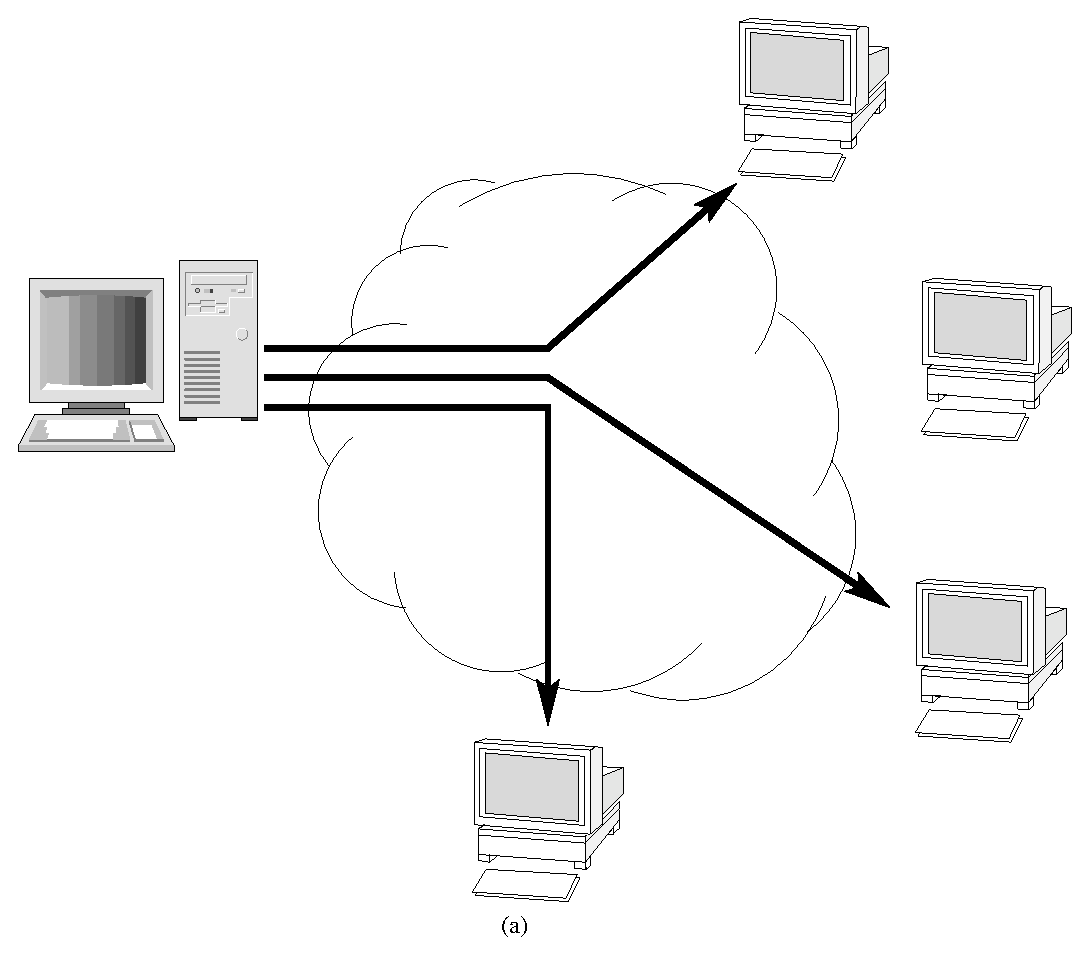
\includegraphics[width=2in]{figures/uniuni.eps}
\hspace{1in}
\includegraphics[width=2in]{figures/unimulti.eps}
\caption{(a) Unicasting the same data to multiple recipients; (b)
Doing the same thing with multicast.\label{unimulti}}
\end{center}
\end{figure}

Or consider a typical case where the sender has a single connection to
the Internet, such as a cable or DSL modem.  Sending the same data to
multiple recipients scattered throughout the Internet with unicast
requires that the same information be sent over that link many times
(\Fig{unimulti}a).  If the sender's first-hop connection has limited
outgoing capacity (say, one 1 Mbps or so), it may not even be
\emph{possible\/} to send some kinds of information---say, a real-time
video stream at 1 Mbps---to more than one recipient without exceeding
the first-hop link capacity, resulting in many lost packets and
poor quality.
%
Clearly it would be more efficient
if the information could be duplicated \emph{after\/} it crosses the first
link, as in \Fig{unimulti}b.
This saves bandwidth \emph{and\/} simplifies life for the sending program.

You may be surprised to learn that the sockets interface over TCP/IP
provides access to services like this---albeit with some
restrictions.  There are two types of
network duplication service: \defn{broadcast} and \defn{multicast}.
With broadcast, the program calls \fcnsys{sendto()}
once and the message is automatically delivered
to \emph{all\/} hosts on the local network.
With multicast, the message is sent once, and delivered
to a specific (possibly empty) \emph{group\/} of hosts throughout the
Internet---namely, those that have
indicated to the network that they should receive messages sent to that group.

\callout{We mentioned that there are some restrictions on these services.
The first is that \emph{only UDP sockets can use broadcast and
multicast services}.  The second is that \emph{broadcast only covers a local
scope}, typically a local area network.
The third restriction is that \emph{multicast across the entire
Internet is presently not supported by most Internet service
providers}.}
In spite of these restrictions, these services can often be useful.
For example, it is often useful to use multicast within a site such
as a campus network, or broadcast to local hosts.

\subsection{Broadcast}

\noindent UDP datagrams can be sent to all nodes on an attached local
network by sending them to a special address.  In IPv4 it is
called the ``limited broadcast address'', and it is the all-ones
address (in dotted-quad notation, 255.255.255.255).
In IPv6 it is called the ``all-nodes address (link scope)'', and has
the value % XXX formatting...
FF02::1.  Routers do not forward packets addressed to either one of
these addresses, so neither one will take a datagram beyond the local
network to which the sender is connected.  Each does,
however, deliver the sent packet to \emph{every\/} node on the
network; typically this is achieved using the hardware broadcast
capability of the local network. (Not all links support broadcast; in
particular, point-to-point links do not.  If
none of a host's interfaces support broadcast, any attempt to use it
will result in an error.)
Note also that a broadcast UDP datagram will actually be ``heard'' at a host
only if some program on that
host is listening for datagrams on the \emph{port\/} to which the
datagram is addressed.

What about a network-wide broadcast address to send a message to all
hosts?  There is no such address.  To see
why, consider the impact on the network of a broadcast to every host on
the Internet.  The send of a single datagram would result in a very, very
large
number of packet duplications by the routers, and bandwidth would be
consumed on each and every network.  The consequences of misuse
(malicious or accidental) are too great, so the designers of IP left
out such an Internet-wide broadcast facility  on purpose.   Even with these
restrictions, broadcast on the local link can be very useful.  Often it is
used in state exchange for network games where the players are all on
the same local area network (e.g., Ethernet).

There is one other difference between a broadcast sender and a regular
sender:  before sending to the broadcast address, the special socket
option \const{so\_broadcast} must be set.  In effect, this asks the
system for ``permission'' to broadcast.
%
We demonstrate the use of
UDP broadcast in \file{BroadcastSender.c}.  Our sender broadcasts 
a given string every three seconds to the limited broadcast address of
the address family indicated by the first argument.

\jcode{BroadcastSender.c}{code/BroadcastSender.c}{1}{1}

\begin{topcode}

\tlcitem{Declare constant address}{9}

Somewhat surprisingly, the all-nodes group address is not defined as a
named system constant, so we give it a name here.

\tlcitems{Parameter processing}{14--19}

\tlcitems{Destination address storage}{20--21}

We use a \type{sockaddr\_storage} structure to hold the destination
broadcast address, since it may be either IPv4 or IPv6.

\tlcitems{Setting up destination address}{24--47}

We set the destination address according to the given type, and
remember the size for later use.  Finally, we save the address in a
pointer to a generic type{sockaddr}.

\tlcitems{Socket creation}{53--56}

\tlcitems{Setting permission to broadcast}{59--63}
By default, sockets cannot broadcast.  Setting the
\const{SO\_BROADCAST} option
for the socket enables socket broadcast.

\tlcitem{Repeatedly broadcast}{65--72}
Send the argument string every three seconds to all hosts on the network.
\end{topcode}

Note that a receiver program does not need to do anything special to
receive broadcast datagrams (except bind to the appropriate port).
Writing a program to receive the broadcasts sent out by
\file{BroadcastSender.c} is left as an exercise.

\subsection{Multicast}

Using multicast is very similar to using unicast, for the sender.
The difference is in the form of the address.
A multicast address identifies a set of receivers who have ``asked''
the network to deliver messages sent to that address.  (This is the
receiver's responsibility; see below.)
A range of the address space is set aside for multicast in both IPv4
and IPv6.  IPv4 multicast addresses are in the range
224.0.0.0 to 239.255.255.255.  IPv6 multicast addresses are those
whose first byte contains 0xFF, i.e., all ones.  The IPv6 multicast
address space has a fairly complicated structure that is mostly beyond
the scope of this book. (The reader is referred to~\cite{RFC4291} for
details.)  For our examples we'll use
addresses beginning with FF1E; they are valid for transient use in global
applications.
(The third hex digit ``1'' indicates a multicast address that
is not permanently assigned for any particular purpose, while the
fourth digit ``E'' indicates global scope.)  An example would be FF1E::1234.

Our example multicast sender, shown in file
\file{MulticastSender.c}, takes a multicast address and
port as an argument, and sends a given string to that address and port
every three seconds.

\jcode{MulticastSender.c}{code/MulticastSender.c}{1}{1}

Note that unlike the broadcast sender, the
multicast sender does not need to set the
permission to multicast.  On the other hand, the multicast sender
may set the \emph{TTL\/} (``time-to-live'') value for the transmitted
datagrams.
Every packet contains a counter, which is initialized to
some default value when the packet is first sent,
and decremented by each router that handles the packet.  
When this counter reaches 0, the packet is discarded.  The TTL mechanism
(which can be changed by setting a socket option) allows us to
control the initial value of this counter, and thus
limit the number of hops a multicast packet can traverse.
For example, by setting TTL=1, the multicast packet  will not
go beyond the local network.

As mentioned above, the multicast network service duplicates and delivers
the message only to a specific set of receivers
This set of receivers, called a
\defn{multicast group}, is identified by a particular
multicast (or group) address.
These receivers need some mechanism to notify the network of
their interest in receiving data sent to a particular multicast
address.  Once notified, the network can begin forwarding the multicast
messages to the receiver.  This notification of the network,
called ``joining a
group,'' is accomplished via a multicast request (signaling)
message sent
 (transparently)
by the underlying protocol implementation.  To cause this to 
happen, the receiving program needs to invoke an
address-family-specific  multicast socket option.
For IPv4 it is  \const{ip\_add\_membership}; for IPv6 it is 
(surprisingly enough) \const{ipv6\_add\_membership}.
This socket option takes a structure containing the address of the
multicast ``group'' to be joined.  Alas, this structure is
also different for the
two versions:
\begin{inlinecode}
struct ip_mreq {
  struct in_addr imr_multiaddr; // Group address
  struct in_addr imr_interface; // local interface to join on
};
\end{inlinecode}
The IPv6 version differs only in the type of addresses it contains:
\begin{inlinecode}
struct ipv6_mreq {
  struct in6_addr ipv6mr_multiaddr; // IPv6 multicast address of group
  unsigned int ipv6mr_interface;    // local interface to join no
  };
\end{inlinecode}
Our multicast receiver contains
a fair amount of  version-specific code to handle the joining process.

\jcode{MulticastReceiver.c}{code/MulticastReceiver.c}{1}{1}

The multicast receiver joins the group, waits to receive a message,
prints it, then exits.

\subsection{Broadcast vs. Multicast}

The decision of using broadcast or multicast in an application
depends on several issues, including the fraction
of network hosts interested in
receiving the data, and the knowledge of the communicating parties.
Broadcast works well if a large percentage of the network hosts wish
to receive the message; however, if few hosts need to receive the
packet, broadcast ``imposes on'' all hosts in the network for the
benefit of a few.
Multicast is preferred, because it limits the duplication of data to
only those that have  expressed interest.
%
The disadvantages of multicast are (i) it is presently not supported globally,
and (ii) the sender and receiver must
agree on an IP multicast address in advance.
Knowledge of an address is not required
for broadcast.  In some contexts (local), this makes broadcast a better
mechanism for discovery than multicast.  All hosts can receive
broadcast by default, so it is simple to ask all hosts a question like
``Where's the printer?''  On the other hand, for wide-area applications,
multicast is the only choice.

\begin{exercises}

\item State precisely the conditions under which an iterative server
is preferable to a multiprocessing server.

\item Would you ever need to implement a timeout in a client or
  server that uses TCP?

\item Why do we make the server socket nonblocking in
\file{UDPEchoServer-SIGIO.c}?  In particular, what bad thing might
happen if we did not?


\item How can you determine the minimum and maximum allowable sizes for
  a socket's send and receive buffers?  Determine the minimums for
  your system.

\item \label{ex:sigpipe} This exercise considers the
reasoning behind the \constsys{sigpipe} mechanism a little further.
Recall that \constsys{sigpipe} is delivered when a program tries  to
send on a TCP socket whose connection has gone away in the meantime.
An alternative approach would be to simply have the \fcn{send()} fail
with \constsys{econnreset}.  Why might the signal-based approach be
better than conveying this information by return value?

\item What do you think will happen if you use the program in
  \file{MulticastReceiver.c} while the program
  \file{BroadcastSender.c} is running on a host connected to the same LAN?

\end{exercises}

\chapter{Under the Hood}
\label{chap:under}%
\newcommand{\netstat}{\texttt{netstat}}

Some of the subtleties of network programming are difficult to grasp
without some understanding of the data structures associated with each
socket in the implementation and certain details of how the underlying
protocols work.  This is especially true of stream (TCP) sockets.
This chapter describes some of what goes on ``under the hood'' when you
create and use a socket.
The initial discussion and Section~\ref{sect:demux} apply to both
datagram (UDP) and stream (TCP) sockets; the rest applies only to TCP
sockets.
Please note that
this description covers only the normal sequence of events and glosses
over many details.  Nevertheless, we believe that even this basic
level of understanding is helpful.  Readers who want the full story
are referred to the TCP specification~[\cite{RFC793}] or to one of the
more comprehensive treatises on the subject~[\cite{ComerV2},
\cite{StevensV2}].

Figure~\ref{fig:structures} is a simplified view of some of the
information associated with a socket---that is, the object created by
a call to \fcn{socket()}.  The integer returned by \fcn{socket()} is
best thought of as a ``handle'' that identifies the collection of data
structures for one communication endpoint that we refer to in this
chapter as the ``socket structure.''
As the figure indicates, more than one
descriptor can refer to the same socket structure.  In fact,
descriptors in \emph{different processes} can refer to the same
underlying socket structure.

\begin{figure}
%\jfigs{figures/ja05f01}{0.7}
\jfigs{figures/structures.eps}{0.5\textwidth}
\caption{\label{fig:structures}Data structures associated with a socket.}
\end{figure}

By ``socket structure'' here we mean all data structures
in the socket layer and TCP implementation that contain state
information relevant to this socket abstraction. 
Thus, the socket structure contains send and receive
queues and other information, including the following:


\begin{itemize}

\item The {local and remote} Internet addresses and port numbers
associated with the socket.  The local Internet address (labeled
``Local IP'' in the figure) is one of those assigned to the local
host; the local port is set at \fcn{bind()} time.
The remote address and port identify the remote
socket, if any, to which the local socket is connected.  We will say
more about how and when these values are determined shortly
(Section~\ref{sect:demux} contains a concise summary).

\item A FIFO queue (``\sque'') of received data waiting to be delivered and a
FIFO queue (``\rque'') for data waiting to be transmitted.

\item For a TCP socket, additional {protocol state} information
relevant to the opening and closing TCP handshakes.  In
Figure~\ref{fig:structures}, the state is ``Closed''; all sockets start
out in the Closed state.
\end{itemize}
Some general-purpose operating systems provide tools that enable users
to obtain a ``snapshot'' of these underlying data structures.
On such tool is \netstat, which is typically available on both
Unix (Linux) and Windows platforms.  Given appropriate options, 
\netstat\ displays exactly the information indicated in
Figure~\ref{fig:structures}: number of bytes in 
\emph{SendQ} and \emph{RecvQ}, 
local and remote IP addresses and port
numbers, and the connection state.
Command-line options may vary, but the output should look something
like this:
\begin{verbatim}
Active Internet connections (servers and established)
Proto Recv-Q Send-Q Local Address           Foreign Address       State      
tcp        0      0 0.0.0.0:36045           0.0.0.0:*             LISTEN     
tcp        0      0 0.0.0.0:111             0.0.0.0:*             LISTEN     
tcp        0      0 0.0.0.0:53363           0.0.0.0:*             LISTEN     
tcp        0      0 127.0.0.1:25            0.0.0.0:*             LISTEN     
tcp        0      0 128.133.190.219:34077   4.71.104.187:80       TIME_WAIT  
tcp        0      0 128.133.190.219:43346   79.62.132.8:22        ESTABLISHED
tcp        0      0 128.133.190.219:875     128.133.190.43:2049   ESTABLISHED
tcp6       0      0 :::22                   :::*                  LISTEN
\end{verbatim}
The first four lines and the last line
depict server sockets listening for connections.
(The last line is a listening socket bound to an IPv6 address.)
The fifth line corresponds to a connection to a web server
(port 80) that is partially shut
down (see Section~\ref{sect:closingTCP} below).
The next-to-last two lines are existing TCP connections.
You may want to play with \netstat, if it is available on your system,
to examine the status of connections in the scenarios depicted below.
Be aware, however, that because the transitions between states
depicted in the figures happen so quickly, it may be difficult to
catch them in the ``snapshot'' provided by \netstat.

Knowing that these data structures exist and how they are affected by
the underlying protocols is useful because they control various
aspects of the behavior of the socket.
For example, because TCP
provides a \emph{reliable} byte-stream service, a copy of any data
sent over a TCP socket must be kept \emph{by the TCP implementation}
until it has been successfully received at the other end of the
connection.
Completion of a call to \fcn{send()} on a TCP socket
does \emph{not}, in general,
imply that the data has actually transmitted---only that it has
been copied into the local buffer.  Under normal conditions it will be
transmitted soon, but the exact moment is under the control of TCP,
not the application.
Moreover, the nature of the
byte-stream service means that message boundaries are \emph{not\/} necessarily
preserved in the input stream.  As we saw in
Section~\ref{sect:framing}, this means that most application protocols
need a \emph{framing\/} mechanism, so the receiver can tell when it has
received an entire message.

On the other hand, with a datagram (UDP) socket, 
packets are
\emph{not} buffered for retransmission, and by the time a call to
\fcn{send}/\fcn{sendto} returns, the data has been
given to the network subsystem for transmission. If the network
subsystem cannot handle the message for some reason, the packet is
silently dropped (but this is rare).

The next three sections deal with some of the subtleties of sending
and receiving with TCP's byte-stream service.  Then,
Section~\ref{sect:lifecycle} considers the connection establishment
and termination of the TCP protocol.  Finally,
Section~\ref{sect:demux} discusses the process of matching incoming
packets to sockets and the rules about binding to port numbers.

\section{Buffering and TCP}
\label{sect:sendrec}%

As a programmer, the most important thing to remember when using a TCP
socket is this:

\begin{quote}
\textbf{You cannot assume any correspondence between
writes to the output stream at one end of the connection
and reads from the input stream at  the other end.}
\end{quote}

In particular, data passed in a single invocation of the output
stream's \fcn{send} method at the sender can
be spread across multiple invocations of the input stream's
\fcn{recv} method at the other end; and a
single \fcn{recv} may return data passed in
multiple \fcn{send}s.

To see this,
consider a program that does the following:
%
\begin{inlinecode}
rv = connect(s,...);
...
rv = send(s, buffer0, 1000, 0);
...
rv = send(s, buffer1, 2000, 0);
...
rv = send(s, buffer2, 5000, 0);
...
close(s);

\end{inlinecode}
%
where the ellipses represent code that sets up the data in the
buffers but contains no other calls to \fcn{send}.
%
This TCP connection transfers 8000 bytes to the receiver.  The way
these 8000 bytes are grouped for delivery at the receiving end of the
connection depends on the timing between the calls to
\fcn{send()} and
\fcn{recv()} at the two ends of the
connection---as well as the size of the buffers provided to the
\fcn{recv()} calls.

We can think of the sequence of all bytes sent (in one direction) on a
TCP connection up to a particular instant in time as being divided into three
FIFO queues:

\begin{enumerate}

\item \emph{\sque}: Bytes buffered in the underlying implementation at
the sender that have been written to the output stream but not yet
successfully transmitted to the receiving host.

\item \emph{\rque}: Bytes buffered in the underlying implementation at
the receiver waiting to be delivered to the receiving program---that
is, read from the input stream.

\item \emph{Delivered}: Bytes already read from the input stream by
the receiver.

\end{enumerate}
%
A call to \fcn{send()} at the sender
appends bytes to \sque.  The TCP protocol is responsible for
moving bytes---in order---from \sque\ to \rque.  It is
important to realize that this transfer cannot be controlled or
directly observed by the user program, and that it occurs in chunks
whose sizes are more or less independent of the size of the buffers
passed in \fcn{send}s.  Bytes are moved from
\rque\ to \emph{Delivered}\ by calls to \fcn{recv()};
the size of the transferred chunks depends on the amount of
data in \rque\ and the size of the buffer given to
\fcn{recv()}.

Figure~\ref{fig:buffers0} shows one possible state of the three queues
\emph{after} the three \fcn{send}s in
the example above, but \emph{before} any
\fcn{in.reads}s at the other end.  The
different shading patterns denote bytes passed in the three different
invocations of \fcn{send()} shown above.

\begin{figure}
%\jfigs{figures/ja05f02}{0.7}
\jfigs{figures/buffers0.eps}{\textwidth}
\caption{\label{fig:buffers0}State of  the three queues after three
  \fcn{send()} calls.}
\end{figure}

The output of \netstat\ on the sending host at the instant depicted in
this figure would contain a line like:
\begin{verbatim}
Active Internet connections
Proto Recv-Q Send-Q Local Address        Foreign Address      State
tcp        0   6500 10.21.44.33:43346    192.0.2.8:22         ESTABLISHED
\end{verbatim}
On the receiving host, \netstat\ shows:
\begin{verbatim}
Active Internet connections
Proto Recv-Q Send-Q Local Address        Foreign Address      State
tcp     1500      0 192.0.2.8:22         10.21.44.33:43346    ESTABLISHED
\end{verbatim}

Now suppose the receiver calls \fcn{recv} with
a byte array of size 2000.  The \fcn{recv} call
will move all of the 1500 bytes present in the waiting-for-delivery
(\rque) queue into the byte array and return the value 1500.
Note that this data includes bytes passed in both the first and second
calls to \fcn{send}.  At some time later,
after TCP has completed transfer of more data, the three partitions
might be in the state shown in Figure~\ref{fig:buffers1}.

\begin{figure}
%\jfigs{figures/ja05f03}{0.7}
\jfigs{figures/buffers1.eps}{\textwidth}
\caption{\label{fig:buffers1}After first \fcn{recv}}
\end{figure}

If the receiver now calls \fcn{recv} with a
buffer of size 4000, that many bytes will be moved from the
waiting-for-delivery (\rque) queue to the already-delivered
(\emph{Delivered}) queue; this includes the remaining 1500 bytes from
the second \fcn{send}, plus the first 2500
bytes from the third \fcn{send}.  The
resulting state of the queues is shown in Figure~\ref{fig:buffers2}.

\begin{figure}
%\jfigs{figures/ja05f04}{0.7}
\jfigs{figures/buffers2.eps}{\textwidth}
\caption{\label{fig:buffers2}After another \fcn{recv}}.
\end{figure}

The number of bytes returned by the next call to
\fcn{recv} depends on the size of the buffer
and the timing of the transfer of data over the network from the
send-side socket/TCP implementation to the receive-side
implementation.  The movement of data from the \sque\ to the
\rque\ buffer has important implications for the design of
application protocols. We have already encountered the need to parse
messages as they are received via a socket
when in-band delimiters are used for framing (see
Section~\ref{sect:framing}).  In the following 
sections, we consider two more subtle ramifications.

\section{Deadlock Danger}
\label{sect:deadlock}%

Application protocols have to be designed with some care to avoid
\emph{deadlock}---that is, a state in which each peer is blocked
waiting for the other to do something.  For example, it is pretty
obvious that if both client and server try to receive immediately
after a connection is established, deadlock will result.  Deadlock can
also occur in less immediate ways.

The buffers \sque\ and \rque\ in the implementation have
limits on their capacity.  Although the actual amount of memory they
use may grow and shrink dynamically, a hard limit is necessary to
prevent all of the system's memory from being gobbled up by a single
TCP connection under control of a misbehaving program.  Because these
buffers are finite, they can fill up, and it is this fact, coupled
with TCP's \emph{flow control} mechanism, that leads to the
possibility of another form of deadlock.

Once \rque\ is full, the TCP {flow control} mechanism kicks in
and prevents the transfer of any bytes from the sending host's
\sque\ until space becomes available in \rque\ as a
result of the receiver calling \fcn{recv()}.
(The purpose of the flow
control mechanism is to ensure that the sender does not transmit more
data than the receiving system can handle.)  A sending program can
continue to call \fcn{send()} until \sque\ is full; however, once
\sque\ is full, a \fcn{send} will block until space
becomes available, that is, until some bytes are transferred to the
receiving socket's \rque.  If \rque\ is also full,
everything stops until the receiving program calls
\fcn{recv} and some bytes are transferred
to \emph{Delivered}.

Let's assume the sizes of \sque\ and \rque\ are
\sqsize\ and \rqsize, respectively.  A
call to \fcn{send()} passing in a buffer of size $n$
such that $n > \sqsize$ will not return until at least
$n-\sqsize$ bytes have been transferred to \rque\ at the
receiving host.  If $n$ exceeds $(\sqsize +\rqsize)$,
\fcn{send()} cannot return until after the
receiving program has read at least $n-(\sqsize +\rqsize)$ bytes
from the input stream.  If the receiving program does not call
\fcn{recv()}, a large
\fcn{send} may not complete successfully.  In
particular, if both ends of the connection call
\fcn{send()} simultaneously, each passing a buffer
bigger than $\sqsize + \rqsize$ bytes,
deadlock \emph{will\/} result: neither write will ever complete, and both
programs will remain blocked forever.

As a concrete example, consider a connection between a program on Host
A and a program on Host B.  Assume \sqsize\ and \rqsize\ are 500
at both A and B.  Figure~\ref{fig:deadlock} shows what happens when
both programs try to send 1500 bytes at the same time.  The first 500
bytes of data in the program at Host A have been transferred to the
other end; another 500 bytes have been copied into \sque\ at
Host A.  The remaining 500 bytes cannot be sent---and therefore
\fcn{send()} will not return---until
space frees up in \rque\ at Host B.  Unfortunately, the same
situation holds in the program at Host B.  Therefore, neither
program's call to \fcn{send()} call will ever return!

\begin{figure}
%\jfigs{figures/ja05f05}{0.7}
\jfigs{figures/deadlock3.eps}{\textwidth}
\caption{\label{fig:deadlock}Deadlock due to simultaneous \fcn{send}s
to output streams at opposite ends of the connection.}
\end{figure}

\begin{quote}
The moral of the story: Design the protocol carefully to avoid
sending large quantities of data simultaneously in both directions.
\end{quote}

% XXXX Removed because this example is only in the Java version! :-(

%% Can this really happen?  Let's review the compression protocol example
%% in Section~\ref{sect:shutdown}.  Try running the compression client
%% with a large file that is still large \emph{after compression}.  The
%% precise definition of ``large'' here depends on your system, but a
%% file that is already compressed and exceeds 2MB should do nicely.  For
%% each read/write, the compression client prints an ``R''/``W'' to the
%% console.  If both the uncompressed and compressed versions of the file
%% are large enough, your client will print a series of Ws and then stop
%% without terminating or printing any~Rs.

%% Why does this happen?  The program \file{CompressClient.java} sends
%% \emph{all} of the uncompressed data to the compression server
%% \emph{before} it attempts to read anything from the compressed stream.
%% The server, on the other hand, simply reads the uncompressed byte
%% sequence and writes the compressed sequence back to the client. (The
%% number of bytes the server reads before it writes some compressed data
%% depends on the compression algorithm it uses.)  Consider the case
%% where \sque\ and \rque\ for both client and server hold
%% 500 bytes each and the client sends a 10,000-byte (uncompressed) file.
%% Suppose also that for this file the server reads about 1000 bytes and
%% then writes 500 bytes, for a 2:1 compression ratio. After the client
%% sends 2000 bytes, the server will eventually have read them all and
%% sent back 1000 bytes, and the client's \rque\ and the server's
%% \sque\ will both be full.  After the client sends another 1000
%% bytes and the server reads them, the server's subsequent attempt to
%% write will block.  When the client sends the next 1000 bytes, the
%% client's \sque\ and the server's \rque\ will both fill up.
%% The next client write will block, creating deadlock.

%% How do we solve this problem?  One solution is to execute the
%% client writing and reading loop in separate threads.  One thread
%% repeatedly reads uncompressed bytes from a file and sends
%% them to the server until the end of the file is reached, whereupon it
%% calls \fcn{shutdown()} on the
%% socket.  The other thread repeatedly reads compressed
%% bytes from the input stream connected to the server
%% and writes them to the output file, until the
%% input stream ends (i.e., the server closes the socket).  When one
%% thread blocks, the other thread can proceed independently.  We can
%% easily modify our client to follow this approach by putting the call
%% to \fcn{SendBytes} in \file{CompressClient.java} inside a thread as
%% follows:

%% \begin{inlinecode}
%% Thread thread = new Thread() \{
%%   public void run() \{
%%     try \{
%%       SendBytes(sock, fileIn);
%%     \} catch (Exception ignored) \{\}
%%   \}
%% \};
%% thread.start();
%% \end{inlinecode}

%% \noindent See \file{CompressClientNoDeadlock.java} on the book's Web
%% site for the complete example.

%% Of course, the problem can be solved without using threads, through
%% the use of nonblocking \class{Channel}s and \class{Selector}s,
%% as described in Chapter~\ref{chap:nio}.

\section{Performance Implications}

The TCP implementation's need to copy user data into \sque\ before
sending it also has implications for performance.  In
particular, the sizes of the \sque\ and \rque\ buffers
affect the throughput achievable over a TCP connection.  ``Throughput''
is the \emph{rate} at which bytes of user data from the sender are
made available to the receiving program; in programs that transfer a
large amount of data, we want to maximize the number of bytes
delivered per second.  In the absence
of network capacity or other limitations, \emph{bigger buffers generally
result in higher throughput}.

The reason for this has to do with the cost of transferring data into
and out of the buffers in the underlying implementation.  If you want
to transfer $n$ bytes of data (where $n$ is large), it is generally
much more efficient to call \fcn{send()} once
with a buffer of size $n$ than it is to call it $n$ times with a
single byte.\footnote{The same thing generally applies to receiving,
although calling \fcn{recv} with a larger buffer does not
guarantee that more data will be returned---in general, only the
data present at the time of a call will be returned.}  However, if you call
\fcn{send()} with a size parameter that is much
larger than \sqsize\ (the size of \sque),
the system has to transfer the data from the
user address space in \sqsize-sized chunks.  That is, the socket
implementation fills up the \sque\ buffer, waits for data to be
transferred out of it by the TCP protocol, refills \sque, waits
some more, and so on.  Each time the socket implementation has to wait
for data to be removed from \sque, some time is wasted in the
form of overhead (a context switch occurs). This overhead is
comparable to that incurred by a completely new call to
\fcn{send()}.  Thus the \emph{effective\/} size
of a call to \fcn{send} is limited by the actual \sqsize.
The same thing applies at the receiving end:
however large the buffer we pass to
\fcn{recv()}, data will be copied out in chunks no
larger than \rqsize, with overhead incurred between chunks.

If you are writing a program for which throughput is an important
performance metric, you will want to change the send and receive
buffer sizes using the  \const{SO\_RCVBUF} and \const{SO\_SNDBUF} socket
options.   Although there is
always a system-imposed maximum size for each buffer, it is typically
significantly larger than the default on modern systems.  Remember
that these considerations apply only if your program needs to send an
amount of data significantly larger than the buffer size, all at once.
Note also that wrapping a TCP socket in a \type{FILE}-stream adds
another stage of buffering and additional overhead, and thus may
negatively affect throughput.

\section{TCP Socket Life Cycle}
\label{sect:lifecycle}%

When a new TCP \type{socket} is created, it cannot be used immediately
for sending and receiving data.  First it needs to be connected to a
remote endpoint.
%
Let us therefore consider in more detail how the underlying structure
gets to and from the connected, or ``Established,'' state.  As we'll
see later, these details affect the definition of
reliability and the ability to bind a socket to a particular port that
was in use earlier.

\subsection{Connecting}
\label{sect:connecting}%

The relationship between the \fcn{connect()} call and
the protocol events associated with
connection establishment at the client are
illustrated in Figure~\ref{fsm0}.  In this and the remaining figures
of this section, the large arrows depict external events that cause
the underlying socket structures to change state.  Events that occur
in the application program---that is, method calls and returns---are
shown in the upper part of the figure; events such as message arrivals
are shown in the lower part of the figure.  Time proceeds left to
right in these figures.  The client's Internet address is depicted as
A.B.C.D, while the server's is W.X.Y.Z; the server's port number is~Q.
(We have depicted IPv4 addresses, but everything here applies to both
IPv4 and IPv6.)
\begin{figure}
%\jfigs{figures/ja05f06}{0.7}
\jfigs{figures/fsm0.eps}{\textwidth}
\caption{\label{fsm0}Client-side connection establishment.}
\end{figure}

When the client calls \fcn{connect()}
with the server's Internet address, W.X.Y.Z, and port, Q,
the underlying implementation creates a socket instance; it is
initially in the Closed state.  If the client did not specify the
local address/port in the constructor call, a local port number (P),
not already in use by another TCP socket, is chosen by the
implementation.  The local Internet address is also assigned; if not
explicitly specified, the address of the network interface through
which packets will be sent to the server is used.  The implementation
copies the local and remote addresses and ports into the underlying
socket structure, and initiates the TCP connection establishment
handshake.

The TCP opening handshake is known as a \emph{3-way handshake} because
it typically involves three messages: a connection request from client
to server, an acknowledgment from server to client, and another
acknowledgment from client back to server.  The client TCP considers
the connection to be established as soon as it receives the
acknowledgment from the server.  In the normal case, this happens
quickly.  However, the Internet is a best-effort network, and either
the client's initial message or the server's response can get lost.
For this reason, the TCP implementation retransmits handshake messages
multiple times, at increasing intervals.  If the client TCP does not
receive a response from the server after some time, it \emph{times
out} and gives up.  In this case \fcn{connect()} returns $-1$ and sets
\var{errno} to \const{ETIMEDOUT}.
The implementation tries very hard to complete the connection before
giving up, and thus it can take on the
order of minutes for a \fcn{connect()} call to fail.
%
After the initial handshake message is sent and before the
reply from the server is received (i.e. the middle part of
Figure~\ref{fsm0}), the output from \netstat\ on the
client host would look something like:

\begin{verbatim}
Active Internet connections
Proto Recv-Q Send-Q Local Address    Foreign Address      State      
tcp        0      0 A.B.C.D:P        W.X.Y.Z:Q            SYN_SENT
\end{verbatim}
where ``\verb+SYN_SENT+'' is the technical name of the client's state
between the first and second messages of the handshake.

If the
server is not accepting connections---say, if there is no program
associated with the given port at the destination---the server-side
TCP will respond (immediately) with a rejection message instead of an
acknowledgment, and \fcn{connect()} returns $-1$ with \var{errno} set
to \const{ECONNREFUSED}.
%
Otherwise, after the client receives a positive reply from the server,
the netstat output would look like:
\begin{verbatim}
Active Internet connections
Proto Recv-Q Send-Q Local Address    Foreign Address      State      
tcp        0      0 A.B.C.D:P        W.X.Y.Z:Q            ESTABLISHED
\end{verbatim}

The sequence of events at the server side is rather different; we
describe it in Figures~\ref{fsm1a}, \ref{fsm1b}, and~\ref{fsm1c}.
The server needs to bind to the particular TCP port
known to the client. Typically, the server specifies only the
port number (here, Q)
in the \fcnsys{bind()} call and gives the special
wildcard address
\const{INADDR\_ANY} for the local IP address.
In case the server host has more than one IP address, this technique allows the
socket to receive connections addressed to any of its IP addresses.
When the server calls \fcn{listen()}, the state of the socket is changed to
``Listening'', indicating that it is ready to accept new connections.
%
These events are depicted in Figure~\ref{fsm1a}.
The output from \netstat\ on the server after this sequence
would include a line like:
\begin{verbatim}
Active Internet connections
Proto Recv-Q Send-Q Local Address    Foreign Address      State      
tcp        0      0 0.0.0.0:Q        0.0.0.0:0            LISTENING
\end{verbatim}
%
Note that any client
connection request that arrives at the server before the
call to \fcn{listen()} will be rejected, even if it arrives
after the call to \fcn{bind()}.

\begin{figure}
%\jfigs{figures/ja05f07}{0.7}
\jfigs{figures/fsm1a.eps}{\textwidth}
\caption{\label{fsm1a}Server-side socket setup.}
\end{figure}

\begin{figure}
%\jfigs{figures/ja05f08}{0.7}
\jfigs{figures/fsm1b.eps}{\textwidth}
\caption{\label{fsm1b}Incoming connection request processing.}
\end{figure}


The next thing the server does is call \fcnsys{accept()}, which
blocks until a connection with a client is established.
We therefore focus in Figure~\ref{fsm1b} on the events that
occur in the TCP implementation when a client connection request
arrives.  Note that everything depicted in this figure happens
``under the covers,'' in the TCP implementation.

When the request for a connection arrives from the client,
a new socket structure is created for the connection.
The new socket's addresses are filled
in based on the arriving packet: The packet's destination  Internet
address and port (W.X.Y.Z and Q, respectively)  become the socket's local
address and port; the packet's source
address and port (A.B.C.D and P)
become the  socket's remote Internet address and port.
Note that the local port number  of the new socket
is always the same as that of the listening socket.
The new socket's state is set to Connecting, and it is added to a list of
not-quite-connected sockets associated with the original server socket.
Note well that the original server socket does not change state.
%
At this point the output of \netstat\ should show \emph{both\/} the original,
listening socket and the newly-created one:
\begin{verbatim}
Active Internet connections
Proto Recv-Q Send-Q Local Address    Foreign Address      State      
tcp        0      0 0.0.0.0:Q        0.0.0.0:0            LISTENING
tcp        0      0 W.X.Y.Z:Q        A.B.C.D:P            SYN_RCVD
\end{verbatim}

In addition to creating a new underlying socket structure, the
server-side TCP implementation sends an acknowledging TCP handshake
message back to the client.  However, the server TCP does not consider
the handshake complete until the third message of the 3-way handshake
is received from the client.  When that message eventually arrives,
the new structure's state is set to ``Established'', and it is then
(and only then) moved to a list of socket structures associated with
the original socket, which represent established connections ready to be
\fcn{accept}ed.
(If the third
handshake message fails to arrive, eventually the ``Connecting''
structure is deleted.)
Output from \netstat\ would then include:
\begin{verbatim}
Active Internet connections
Proto Recv-Q Send-Q Local Address    Foreign Address      State      
tcp        0      0 0.0.0.0:Q        0.0.0.0:0            LISTENING
tcp        0      0 W.X.Y.Z:Q        A.B.C.D:P            ESTABLISHED
\end{verbatim}

Now we can consider (in Figure~\ref{fsm1c}) what happens when the
server program calls \fcn{accept()}.
The call unblocks as soon as there is something in the listening
socket's list of new connections. 
(Note that this list may already be non-empty when \fcn{accept()}
is called.)  At that time, the new socket structure is removed from the list,
and a socket descriptor is allocated and returned as the result of
\fcn{accept()}.

\begin{figure}
%\jfigs{figures/ja05f09}{0.7}
\jfigs{figures/fsm1c.eps}{\textwidth}
\caption{\label{fsm1c}\fcn{accept}}
\end{figure}

It is important to note that each structure in the
server socket's associated list
represents a fully established TCP connection with a client at the
other end.  Indeed, the client can send data as soon as it receives
the second message of the opening handshake---which may be long before
the server accepts the client connection!

\subsection{Closing a TCP Connection}
\label{sect:closingTCP}%

TCP has a \emph{graceful close} mechanism that allows applications to
terminate a connection without having to worry about loss of data that
might still be in transit.  The mechanism is also designed to allow
data transfers in each direction to be terminated independently.
% XXXXX FIXME: COMPRESSION EXAMPLE
% as in
% the [FIX: compression] example of Section~\ref{sect:shutdown}.
It works like
this: the application indicates that it is finished sending data on a
connected socket by calling \fcn{close()} or by
calling \fcn{shutdown()}.  At
that point, the underlying TCP implementation first transmits any data
remaining in \sque\ (subject to available space in
\rque\ at the other end), and then sends a closing TCP
handshake message to the other end.  This closing handshake message
can be thought of as an end-of-stream marker: it tells the
receiving TCP that no more bytes will be placed in \rque.
(Note that the closing handshake message itself is \emph{not} passed
to the receiving application, but that its position in the byte stream
is indicated by \fcn{recv} returning $-1$.)  The closing TCP waits
for an acknowledgment of its closing handshake message, which
indicates that all data sent on the connection made it safely to
\rque.  Once that acknowledgment is received, the connection is
``Half closed.''
%
The connection is not \emph{completely} closed until a symmetric
handshake happens in the other direction---that is, until \emph{both}
ends have indicated that they have no more data to send.

\begin{figure}
%\jfigs{figures/ja05f10}{0.7}
\jfigs{figures/fsm2.eps}{\textwidth}
\caption{\label{fsm2}Closing a TCP connection first.}
\end{figure}

The closing event sequence in TCP can happen in two ways: either one
application calls \fcn{close()} (or
\fcn{shutdown()}) and completes
its closing handshake before the other calls
\fcn{close/shutdown}, or both close
simultaneously, so that their
closing handshake messages cross in the network.  Figure~\ref{fsm2}
shows the sequence of events in the implementation when the
application invokes \fcn{close()} \emph{before\/}
the other end closes.  The closing handshake message is sent, the
state of the socket structure is set to ``Closing'', and the call
returns.
After this point, further attempts to perform any operation on the
socket result in error returns. % XXXX
When the acknowledgment for the close handshake is
received, the state changes to ``Half closed'', where it remains until
the other end's close handshake message is received.
At this point the output of \netstat\ on the
client would show the status of the connection as:
\begin{verbatim}
Active Internet connections
Proto Recv-Q Send-Q Local Address    Foreign Address      State      
tcp        0      0 A.B.C.D:P        W.X.Y.Z:Q            FIN_WAIT_2
\end{verbatim}
(\verb+FIN_WAIT_2+ is the technical name for the ``half-closed'' state at
the host that initiates close first.  The state denoted by ``closing''
in the figure is technically called \verb+FIN_WAIT_1+,
but it is transient and is difficult to catch with \netstat.)
Note that if the
remote endpoint goes away while the connection is in this state, the
local underlying structure will stay around indefinitely.  Otherwise,
when the other end's close handshake message arrives an
acknowledgment is sent and the state is changed to ``Time-Wait''.
Although the descriptor in the application
program may have long since been reclaimed (and even reused),
the associated underlying
socket structure continues to exist in the implementation for a minute or
more; the reasons for this are discussed on
page~\pageref{time-wait-state}.

\begin{figure}
%\jfigs{figures/ja05f11}{0.7}
\jfigs{figures/fsm3.eps}{\textwidth}
\caption{\label{fsm3}Closing after the other end closes.}
\end{figure}
The output of \netstat\ at the right end of Figure~\ref{fsm2} 
includes:
\begin{verbatim}
Active Internet connections
Proto Recv-Q Send-Q Local Address    Foreign Address      State      
tcp        0      0 A.B.C.D:P        W.X.Y.Z:Q            TIME_WAIT
\end{verbatim}

Figure~\ref{fsm3} shows the simpler sequence of events at the endpoint
that does not close first.  When the closing handshake message
arrives, an acknowledgment is sent immediately, and the connection
state becomes ``Close-Wait.''
The output of \netstat\ on this host shows:
\begin{verbatim}
Active Internet connections
Proto Recv-Q Send-Q Local Address    Foreign Address      State      
tcp        0      0 W.X.Y.Z:Q        A.B.C.D:P            CLOSE_WAIT
\end{verbatim}
%
At this point, it's all over: the implementation is just
waiting for the application to call \fcn{close()}.
When it does, the socket descriptor is deallocated and the final close
handshake is initiated. When it completes, the underlying socket structure is 
deallocated.

Although most applications use \fcn{close()}, \fcn{shutdown()}
actually provides more flexibility.  A call to \fcn{close()}
terminates \emph{both\/} directions of transfer and causes the file
descriptor associated with the socket to be deallocated.
Any undelivered data remaining in \rque\ is
discarded, and the flow control mechanism prevents any further
transfer of data from the other end's \sque.  All trace of the socket
disappears from the calling program.
Underneath, however, the associated socket structure continues to exist
until the other end initiates its closing handshake.
A program calling \fcn{shutdown()} with second argument
\const{SHUT\_WR} can continue to receive data on
the socket; only sending is prohibited.
The fact that the other end of the connection has closed is
indicated by \fcn{recv()} returning $0$ (once \rque\ 
is empty, of course)
to indicate that there will be no more data available on the connection.

In view of the fact that both \fcn{close()} and
\fcn{shutdown()} return without
waiting for the closing handshake to complete, you may wonder how the
sender can be assured that sent data has actually made it to the
receiving program (i.e., to \emph{Delivered}).  In fact, it is
possible for an application to call
\fcn{close()} or
\fcn{shutdown()} and have it
complete successfully (i.e., not return $-1$) \emph{while there
is still data in \sque}.  If either end of the connection then crashes
before the data makes it to \rque, data may be lost without the
sending application knowing about~it!

\callout{The best solution is to design the application protocol so that
whichever side closes first, does so
\emph{only after} receiving application-level assurance that its data
was received.}  For example, when our \file{TCPEchoClient.c} program
receives the same number of bytes as it sent, there should be nothing
more in transit in either direction, so it is safe for it to close the
connection.  (Note that there is no \emph{guarantee\/} that the bytes
received were those sent; the client is assuming that the server
implements the ``echo'' protocol.  In a real application the client
should certainly \emph{not\/} trust the server to ``do the right thing''.

The other solution is to modify the semantics of \fcn{close()}
by setting the \const{SO\_LINGER} socket option before
calling it.  The \const{SO\_LINGER} option specifies an amount of time
for the TCP
implementation to wait for the closing handshake to complete.  The
setting of \const{SO\_LINGER} and the specification
of the wait time is given to \fcn{setsockopt()} using the
\type{linger} structure:

\begin{inlinecode}
struct linger {
    int  l_onoff;   // Nonzero to linger
    int  l_linger;  // Time (secs.) to linger
};
\end{inlinecode}

\noindent To use the linger behavior, set \param{l\_onoff} to a
nonzero value and specify the time to linger in \param{l\_linger}.
When \const{SO\_LINGER} is set,
\fcn{close()} blocks \emph{until the
closing handshake is completed\/} or until the specified amount of time
passes.  If the handshake does not complete in time,
an error indication (\const{ETIMEDOUT}) is returned.
Thus, if \const{SO\_LINGER} is set and
\fcn{close()} returns no error, the
application is assured that everything it sent reached \rque.

At the
time of this writing, however, \fcn{close()} provides no indication
that the closing handshake failed to complete, even if the time limit
set by \fcn{setSoLinger} expires before the closing sequence
completes.  In other words, \fcn{setSoLinger} does not provide any
additional assurance to the application in current implementations.

The final subtlety of closing a TCP connection revolves around the
need for the Time-Wait state\label{time-wait-state}.  The TCP
specification requires that when a connection terminates, at least one
of the sockets persists in the Time-Wait state for a period of time
after both closing handshakes complete.  This requirement is motivated
by the possibility of messages being delayed in the network.  If both
ends' underlying structures go away as soon as both closing handshakes
complete, and a \emph{new} connection is immediately established
between the same pair of socket addresses, a message from the previous
connection, which happened to be delayed in the network, could arrive
just after the new connection is established.  Because it would
contain the same source and destination addresses, the old message
could be mistaken for a message belonging to the new connection, and
its data might (incorrectly) be delivered to the application.

Unlikely though this scenario may be, TCP employs multiple mechanisms
to prevent it, including the Time-Wait\ state.  The Time-Wait\ state
ensures that every TCP connection ends with a quiet time, during which
no data is sent.  The quiet time is supposed to be equal to twice the
maximum amount of time a packet can remain in the network.  Thus, by
the time a connection goes away completely (i.e., the socket structure
leaves the Time-Wait\ state and is deallocated) and clears the way for
a new connection between the same pair of addresses, no messages from
the old instance can still be in the network.  In practice, the length
of the quiet time is implementation dependent, because there is no
real mechanism that limits how long a packet can be delayed by the
network.  Values in use range from 4~minutes down to 30~seconds or
even shorter.

The most important consequence of Time-Wait\ is that as long as the
underlying socket structure exists, no other socket is permitted to
bind to the same local port.  (More on this below.)

\section{Demultiplexing Demystified}
\label{sect:demux}%

The fact that different sockets on the same machine can have the same
local address and port number is implicit in the discussions above.
For example, on a machine with only one IP address, every
new socket \fcn{accept()}ed via a listening socket
will have the same local address and port number
as the listening socket.  
Clearly the process
of deciding to which socket an incoming packet should be
delivered---that is, the \emph{demultiplexing} process---involves
looking at {more} than just the packet's destination address and port.
Otherwise there could be ambiguity about which socket an incoming
packet is intended for.  The process of matching an incoming packet to
a socket is actually the same for both TCP and UDP, and can be
summarized by the following points:
\begin{itemize}
\item The local port
in the socket structure \emph{must} match the destination port number
in the incoming packet.
\item Any address fields in the socket
structure that contain the wildcard value (*) are considered to match
\emph{any} value in the corresponding field in the packet.
\item If there is more than one socket structure that matches an incoming
packet for all four address fields, the one that matches using the
fewest wildcards gets the packet.
\end{itemize}

For example, consider a host with two IP addresses, 10.1.2.3 and
192.168.3.2, and with a subset of its active TCP socket structures, as
shown in Figure~\ref{demuxex}.  The structure labeled 0 is associated
with a listening socket and has port 99
with a wildcard local address.  Socket structure~1 is also for a
listening socket on the same port, but
with the local IP address 10.1.2.3 specified (so it will only accept
connection requests to that address).  Structure~2 is for a connection
that was accepted via structure 0's listening socket, and
thus has the same local port number (99), but also has its local and remote
Internet addresses filled in.  Other sockets belong to other active
connections.  Now consider a packet with source IP address
172.16.1.10, source port 56789, destination IP address 10.1.2.3, and
destination port 99.  It will be delivered to the socket associated
with structure 1, because that one matches with the fewest wildcards.

\begin{figure}
%\jfigs{figures/ja05f12}{0.7}
\jfigs{figures/demuxex.eps}{\textwidth}
\caption{\label{demuxex}Demultiplexing with multiple matching sockets.}
\end{figure}

When a program attempts to \fcnsys{bind()} to a particular local port
number, the existing sockets are checked to make sure that no socket
is already using that local port.  The call to \fcn{bind()} will fail
and set \const{EADDRINUSE}  if \emph{any} socket matches the local
port and local IP address (if any) specified in the argument to \fcn{bind()}.
This can cause problems in the following scenario:
%
\begin{enumerate}

\item A server's listening socket is bound to some particular port
  $P$.

\item The server accepts a connection from a client, which enters the
  Established state.

\item The server terminates for some reason---say, because the
  programmer has created a new version and wants to test it.
  When the server program exits,
  the underlying system automatically (and virtually) calls
 \fcn{close()} on  all of its existing sockets.  The socket that was
  in the Established state immediatey  transitions to the Time-Wait state.

\item
The programmer starts up a new instance of the server, which attempts
to \fcn{bind()} to port $P$.
\end{enumerate}
Unfortunately the new server's call to \fcnsys{bind()} will fail with
EADDRINUSE because of the old socket in Time-Wait state.

As of this writing, there are two ways around this.  One
is to wait until the underlying structure leaves the
Time-Wait\ state.  The other is for the server to set the
\const{SO\_REUSEADDR} socket option  \emph{before\/} calling
\fcn{bind()}. That lets \fcn{bind()} succeed in spite of the existence
of any sockets representing earlier connections to the server's port.
%
There is no danger of ambiguity, because the existing connections
(whether still in the Established or Time-Wait\ state) have remote
addresses filled in, while the socket being bound does not.
In general, the \const{SO\_REUSEADDR} option also
enables a socket
to bind to a local port to which another socket is already bound,
provided that the IP address to which it is
being bound (typically the wildcard \const{INADDR\_ANY}
address)
is different from the existing socket's.
The default \fcnsys{bind()} behavior is to disallow such requests.

\begin{exercises}

\item The TCP protocol is designed so that simultaneous connection
attempts will succeed.  That is, if an application using port P and
Internet address W.X.Y.Z attempts to connect to address A.B.C.D, port
Q, at the same time as an application using the same address and port
tries to connect to W.X.Y.Z, port P, they will end up connected to
each other.  Can this be made to happen when the programs use the
sockets API?

\item The first example of ``buffer deadlock'' in this chapter
involves the programs on {both} ends of a connection trying to send
large messages.  However, this is not necessary for deadlock.  How
could the \file{TCPEchoClient} from earlier chapters be made
to deadlock when 
it connects to the \file{TCPEchoServer} from that chapter?

\end{exercises}

% OUTLINE
% 1. Purpose of the chapter
% 2. Overview of the socket wrapper library
% 3. Plus one service
% 3.1 Server Description
% 3.2 Client Description
% 3.3 Running client and server
% 4. Survey Service
% 4.1 Support functions
% 4.2 Server description
% 4.3 Client description
% 4.4 Running client and server
% 5 Enhanced server
% 5.1 SocketAddress
% 5.2 iostream interface
% 5.3 Server description
% 5.4 Client description
% 5.5 Administrative client description
% 5.6 Running server and the clients
	
\chapter{Socket Programming in C++}
\label{chap:cpp}

\vspace{-0.3in}
\textbf{(contributed by David B.\ Sturgill)}

\vspace{-0.2in}
{\Large {\bf David B. Sturgill}}
\vspace{0.3in}

This book is for people who want to understand sockets.  It's for
people who want to know not only how to get a couple of programs to
communicate over a network but also how and why the sockets API works
like it does.  Or course, lots of developers use sockets all the time
without really understanding these details.  It's common to use
sockets via a library that offers a simplified interface to socket
creation, name resolution and message transmission.  This is
particularly common in object-oriented languages like C++ and Java,
where it's easy to wrap socket functionality in a collection of
related classes.

The PracticalSocket library was developed to help expose students to
the basics of socket programming without requiring a complete
understanding of some of the material covered elsewhere in this book.
This library is typical of object-oriented wrappers around socket
functionality; it tries to offer a simple interface to the most
commonly used functionality.  The PracticalSocket library provides
portability between Windows and Unix platforms, and it can serve an
instructional purpose since its source code is readily available.

A reader who is more comfortable in C or who prefers to start by
understanding what's going on underneath should save this chapter for
last.  It can serve as a summary and application of many of the
concepts introduced earlier.  For a reader who is an experienced C++
programmer or who prefers to learn about sockets more selectively,
this chapter can be read earlier and can serve as an overview of
concepts covered in much more detail in earlier chapters.  The
examples presented here include many pointers to appropriate sections
earlier in the text, so this chapter can serve as an entry point for
many other sections of the book.

In this chapter, we introduce the PracticalSocket library and
demonstrate its use in a simple application.  Through a series of more
sophisticated applications, we expose additional features of the
library and demonstrate how PracticalSockets or a similar library
might be used in practice.  Both the PracticalSocket library and the
example programs used in this chapter to demonstrate it are available
from the website for this text.

\section{PracticalSocket Library Overview}

\noindent
Figure~\ref{fig:Inheritance} illustrates the classes in
PracticalSockets and their inheritance relationships.  All the classes
ending in ``Socket'' serve as wrappers around TCP or UDP sockets and
provide a simple interface for creating a socket and using it for
communication.  The \type{SocketException} class provides support for
error handling, and \type{SocketAddress} serves as a wrapper around an
address and port number.

\begin{figure}[htbp]
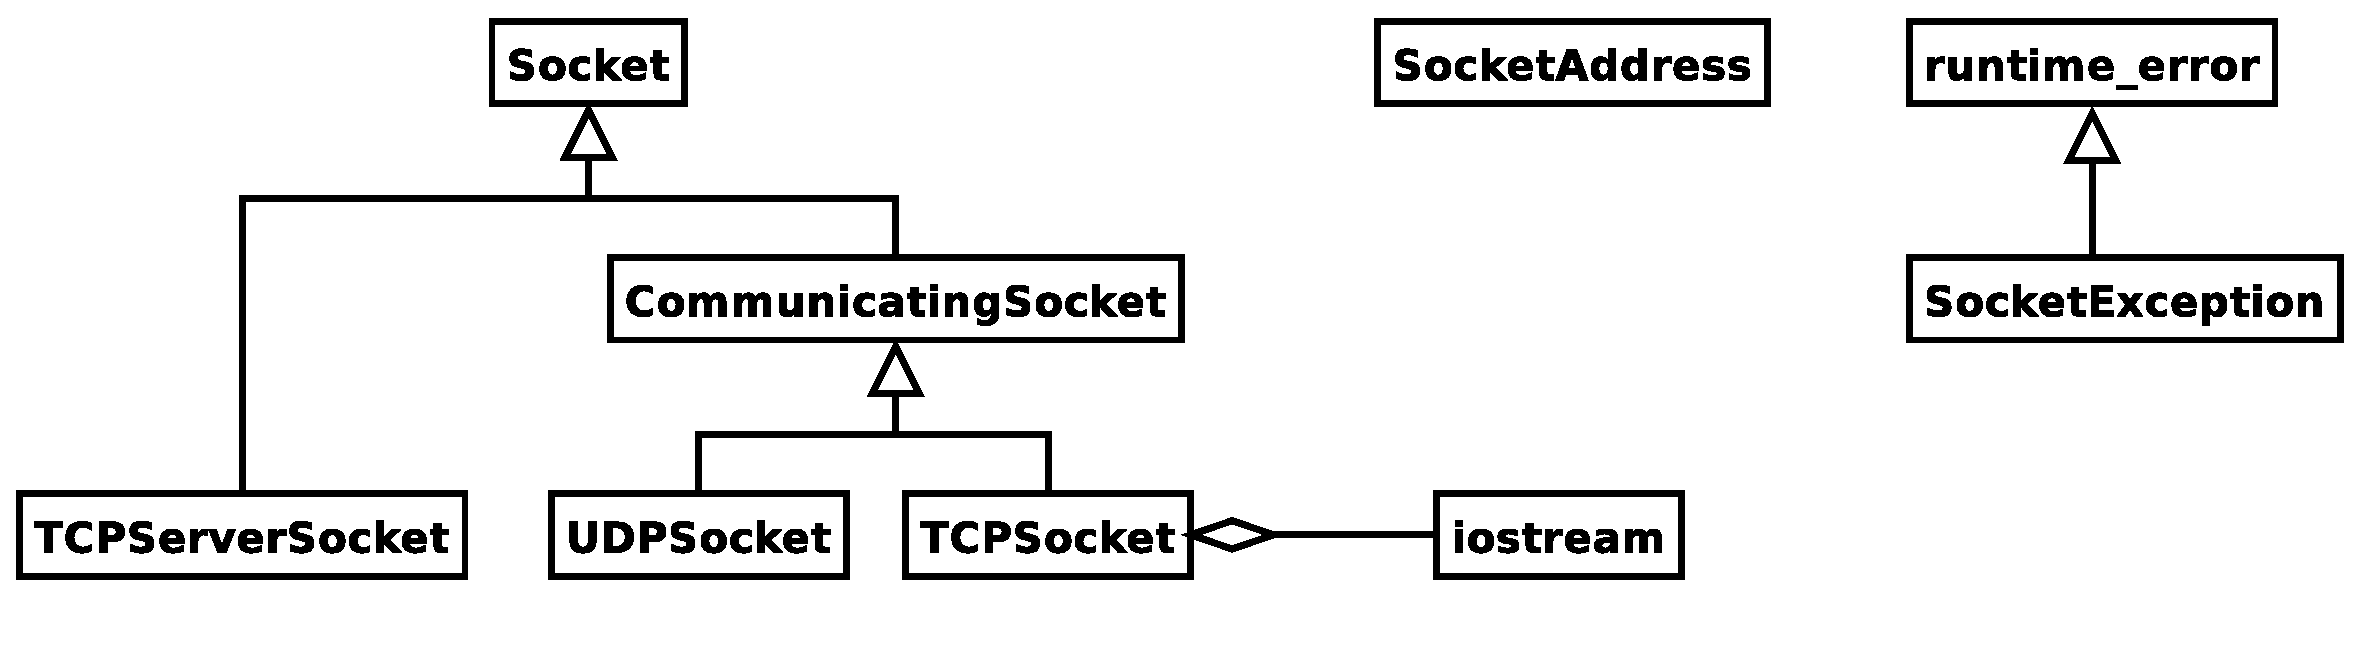
\includegraphics[width=5.5in]{figures/Inheritance.eps}
\caption{\label{fig:Inheritance}PracticalSockets Class Diagram}
\end{figure}

We can get started using this library without understanding everything
about its classes and methods all at once.  We'll start by covering
just enough to write a simple application.  From there, we can
introduce new features gradually.

The \type{TCPSocket} class is the basic mechanism for communication
over TCP.  It is implemented as wrapper around a TCP socket and serves
as an endpoint in a bidirectional communication channel.  If two
applications want to communicate, they can each obtain an instance of
\type{TCPSocket}.  Once these two sockets are connected, sequences of
bytes sent from one can be received at the other.

Functionality for \type{TCPSocket} is distributed across the class
itself and its two base classes, \type{CommunicatingSocket} and
\type{Socket}.  The \type{Socket} class is at the top of the
inheritance hierarchy, and contains only functionality common to all
socket wrappers.  Among other things, it has the job of keeping up
with the underlying socket descriptor, and it automatically closes its
descriptor when it is destroyed.

The \type{CommunicatingSocket} class is an abstraction for a socket
that, once connected, can exchange data with a peer socket.  It
provides \fcnref{send()} and \fcnref{recv()} methods that are wrappers
around the \fcnrefsys{send()} and \fcnrefsys{recv()} calls for the
underlying socket descriptor.  A successful call to the
\fcnref{send()} method of a \type{CommunicatingSocket} will send the
first \param{bufferLen} bytes pointed to by \param{buffer} to the peer
\type{CommunicatingSocket}.  A call to the \fcnref{recv()} method of a
\type{CommunicatingSocket} will attempt to read up to
\param{bufferLen} bytes of data from the peer and store the result in
the memory pointed to by \param{buffer}.  The \fcnref{recv()} method
will block until data is available on the socket, and it will return
the number of bytes received on the socket and written into \param{buffer}.
After a socket is closed, \fcnref{recv()} will return zero to indicate
that no more data can be received.

\begin{inlinefcn}
\type{void} \type{CommunicatingSocket}::\fcnref{send}(\type{const void *}\param{buffer},
\type{int} \param{bufferLen}) throw(\type{SocketException});\\
\type{int} \type{CommunicatingSocket}::\fcnref{recv}(\type{void *}\param{buffer}, \type{int}
\param{bufferLen}) throw(\type{SocketException});\\
\type{int} \type{CommunicatingSocket}::\fcnref{recvFully}(\type{void *}\param{buffer}, \type{int}
\param{bufferLen}) throw(\type{SocketException});
\end{inlinefcn}

The stream of bytes transmitted between sockets may be fragmented into
packets and reconstituted by buffering on its way from the sender to
the receiver.  \callout{A group of bytes sent in a single call to
\fcnref{send()} may not all be received in a single, corresponding
call to \fcnref{recv()}}.  The \fcnref{recvFully()} method is intended
to help with this.  It works just like \fcnref{recv()}, except that it
blocks until either exactly \param{bufferLen} bytes are received or
the socket is closed.  The return value from \fcnref{recvFully()}
reports the number of bytes received.  Ordinarily, this will be the
same as \param{bufferLen}.  However, if the socket is closed before
all the requested bytes are transmitted, a value less than
\param{bufferLen} may be returned.

The PracticalSocket library uses C++ exceptions to report when
something goes wrong.  This is evident in the prototypes above.  An
instance of \type{SocketException} is thrown whenever an error occurs
in the library.  This exception object inherits from
\typesys{runtime\_error}, so it can be caught as an instance of
\type{SocketException} by error handling code specific to the
communications portion of an application.  A \type{SocketException}
may be caught as a more general exception type by more general
error-handling code.  The \fcnrefsys{what()} method of a
\type{SocketException} returns a string with a short description of
the particular error that occurred.

The way to obtain an instance of \type{TCPSocket} depends on the role
of the application.  To establish a pair of connected \type{TCPSocket}
peers, one application must function as a server and the other as a
client.  The server listens for new connections by creating an
instance of \type{TCPServerSocket}.  The other creates a
\type{TCPSocket} directly.  The \type{TCPServerSocket} class is
derived from \type{Socket}, but not \type{CommunicatingSocket}.  It is
used to establish new TCP socket connections with client applications,
but isn't, itself, used to send and receive bytes.  The server must
construct a \type{TCPServerSocket} with an application-defined port
number.  Afterward, a call to \fcnref{accept()} will block until a
client application attempts to connect by creating a \type{TCPSocket}
with the same port number.  When this happens, \fcnref{accept()}
will return a pointer to a new instance of \type{TCPSocket} that is
connected to the \type{TCPSocket} peer on the client.

\begin{inlinefcn}
\fcnref{TCPServerSocket}(\type{unsigned short}localPort) 
      throw(\type{SocketException});\\
\type{TCPSocket *}\type{TCPServerSocket}::\fcnref{accept}() 
throw(\type{SocketException});
\end{inlinefcn}

The client application creates its end of the socket connection by
simply constructing an instance of \type{TCPSocket} and providing the
name or address of the server's host and the same port number.  Once a
pair of connected \type{TCPSocket} objects have been created, client
and server can communicate using the \fcnref{send()} and
\fcnref{recv()} methods until one of the endpoints closes its
connection via the destructor or the \fcnref{close()} method.

\begin{inlinefcn}
\fcnref{TCPSocket}(\type{const char *}\param{foreignAddress},
\type{in\_port\_t} \param{foreignPort})
throw(\param{SocketException});\\
\type{void} \type{Socket}::\fcnref{close}();
\end{inlinefcn}

\section{Plus One Service}

The few classes and methods introduced so far are enough to let us
implement a simple client and server similar to the ones in previous
chapters.  Here, accessing sockets through the PracticalSocket
classes yields somewhat shorter source code that hides many of the
details of the underlying API.  The ``plus one'' service is a
client-server application that performs the increment operation.  The client
sends an unsigned integer to the server and the server sends back a
value that's one greater.

\subsection{Plus One Server}

\file{PlusOneServer.c} is the server portion of the application.  It
accepts client connections, reads a 32-bit unsigned integer from each
client, increments it and then sends it back.

\jcode{PlusOneServer.cpp}{practical/PlusOneServer.cpp}{1}{1}

\begin{topcode}


\tlcitems{Application setup}{1--6}

Access to the sockets API is hidden behind the PracticalSocket
classes.  The application only needs to include the header for the
library and any calls we use directly.


\tlcitems{Error handling}{8, 25--27}

Error handling is via exceptions.  If an error occurs, it is caught at
the end of the main function, and the program prints an error message
before terminating.

\tlcitem{Create a server socket}{9}

The server creates a \type{TCPServerSocket} that listens for
connections on port 9431.  When constructed like this, the
\type{TCPServerSocket} automatically makes the calls to
\fcnref{socket()}, \fcnref{bind()} and \fcnref{listen()} described in
Sections~\ref{sect:connectingASocket}, \ref{sect:bindingToAnAddress}
and \ref{sect:handlingIncomingConnections}.  If anything goes wrong in
one of these steps, an exception is thrown.

To keep the example simple, the server's port number is hard-coded in
the constructor call.  Of course, it would be more maintainable to use
a named constant in a header file as the port number.

\tlcitems{Repeatedly accept client connections}{12--13}

The server repeatedly calls the \fcnref{accept()} method to wait for a
new client connection.  When a client connects, this method returns a
pointer to a new \type{TCPSocket} for communicating with the client.
This method is a wrapper around the \fcnref{accept()} call described
in Section~\ref{sect:handlingIncomingConnections}.  If something goes
wrong in \fcnref{accept()}, the catch block reports the error and the
program terminates.

\tlcitems{Read an integer from the client and convert byte order}{15--17}

Client and server have been written to exchange fixed-sized messages
in the form of unsigned 32-bit integers.  The server uses a
stack-allocated integer, \var{val}, to hold the received message.
Since the server is expecting a four-byte message, it uses the
\fcnref{recvFully()} method of \type{TCPSocket} to read the message
directly into the storage for \var{val}.  If the client connection is
closed before the entire message arrives, \fcnref{recvFully()} returns
fewer than the expected number of bytes and the server ignores the
message.

Although client and server agree on the size of a message, if they are
running on different hosts, they may represent integers using
different byte orders.  To take care of this possibility, we agree to
only transmit values that are in big-endian byte order.  The server
uses \fcnref{ntohl()} to convert the received integer to local byte
order if necessary.  

Concerns over reading entire messages and adjusting byte order are
really just the issues of framing and encoding.
Chapter~\ref{chap:encoding} focuses specifically on these topics and
offers a variety of techniques for handling framing and encoding.

\tlcitems{Increment the client integer and send it back}{18--20}

The server adds one to the client-provided value and then converts it
back to network byte order.  The server sends the value back to
the client by sending a copy of the four bytes of memory used to
represent \var{val}.

\tlcitem{Close client connection}{22}

When the server destroys its instance of \type{TCPSocket}, the
socket connection is closed.  If the server had neglected
to destroy this object, it would have not only leaked memory but also
leaked an underlying socket descriptor with each client connection.  A
server with this type of bug could very quickly reach an
operating-system-enforced limit on per-process resources.

\end{topcode}

\subsection{Plus One Client}

\file{PlusOneClient.c} is the client counterpart of the plus one
server.  It connects to the server, sends it a copy of an integer
value given on the command line, and prints out the value the server
sends back.

\jcode{PlusOneClient.cpp}{practical/PlusOneClient.cpp}{1}{1}

\begin{topcode}

\tlcitems{Application setup and parameter checking}{1--12}

The client uses the PracticalSocket classes along with support from a
few other header files.  On the command line, the client expects an
address or hostname for the server and an integer value to send to the
server.  A usage message is printed if the wrong number of arguments is given.

\tlcitems{Error handling}{14, 27--29}

As in the server, a socket-related exception is caught by code at the
end of the program, and an error message is printed.

\tlcitem{Connect to the server}{14}

The client creates an instance of \type{TCPSocket}, passing in the
user-supplied hostname and the hard-coded port number for the server.
This constructor hides a lot of detail in the underlying sockets API.
First, the given hostname is resolved to one or more addresses.  As
<<<<<<< cpp.tex
described in Chapter~\ref{sect:address-independence}, the
=======
described in Chapter~\ref{chap:addrindep}, 
>>>>>>> 1.6
\fcnref{getaddrinfo()} returns all matching addresses for a given host
and port.  Some may be IPv4 addresses, and some may be IPv6.  The
\type{TCPSocket} constructor creates a socket for the first address and
attempts to connect to it.  If this fails, each successive address is
tried until a connection can be established.  If no addresses will
connect, an exception is thrown.

\tlcitems{Parse, convert and send value to server}{17--19}

The client parses the user-provided value from the command line,
converts it to network byte order and sends it to the server by
sending the four bytes starting at the value's starting address.


\tlcitems{Receive incremented value, convert and print}{22--25}

Using \fcnref{recvFully()}, the client blocks until it either receives a
four-byte integer from the server or the socket connection is closed.
If all four bytes arrive, the received value is converted to
host byte order and printed.

\tlcitem{Close the socket}{25}

Since the client's \type{TCPSocket} is allocated on the stack, it is
automatically closed and destroyed when the socket goes out of scope.

\end{topcode}

\subsection{Running Server and Client}

The executable \exec{PlusOneServer} requires no command-line
arguments.  Once compiled, it should be started from the command
prompt and permitted to run for as long as you want to try it out.
While the server is running, you should run a copy of
\exec{PlusOneClient} from a different command prompt, possibly on a
different host.  Supply the name of the server's host and an integer
value on the command line and it should, with a little help from the
server, produce a value one larger than the command-line argument.
For example, if the server is running on a host named ``venus,'' you
should be able to run the client as follows:

\noindent \textbf{PlusOneClient connecting to a server on host, venus}
\begin{shell}
\prompt \typed{PlusOneClient venus 345318} \\
\response{Server Response: 345319}
\end{shell}

\begin{exercises}

\item Instead of simply incrementing the value from a single client,
  modify the server so it will send back the sum of two values
  supplied by different clients.  After a first client connects, the
  server will wait for a second client.  The server will read integer
  values from both clients and send back the sum of these two values
  to both.

\item The client and server communicate using binary-encoded,
  fixed-sized messages.  Modify these programs so that they use
  variable-length, text-encoded messages as described in
  Section~\ref{sect:textEncoding}.  The sender will write its integer
  value to character array as a sequence of ascii-encoded digits.  The
  receiver will read a copy of this array and parse out the integer.

\end{exercises}

\section{Survey Service}

Building on the concepts demonstrated in the plus one service and
using techniques presented in Chapters~\ref{chap:encoding} and
\ref{chap:advanced}, we can create a distributed application that does
something a little more useful.  The survey client and server
implement a simple, distributed survey application.  At startup, the
server reads a list of survey questions and responses from a text
file.  When a client connects, the server sends it copies of the
questions and response options.  The client prints each question and
sends the user's response back to the server, where it is recorded.

The file, \file{survey1.txt}, is an example survey file the server
might use.  The first line gives the number of questions.  This is
followed by a description for each question.  A question is described
by a one-line prompt, followed by a line giving the number of
responses and a line of text for each response.  For example, the
first question on the survey below is ``What is your favorite flavor
of ice cream?''  The three possible responses are ``Vanilla,''
``Chocolate'' or ``Strawberry.''  As users take the survey, the server
will keep up with how many selected each of these responses.

\jcode{survey1.txt}{practical/survey1.txt}{1}{1}

\subsection{Survey Support Functions}

The client and server depend on common functionality implemented in
\file{SurveyCommon.h} and \file{SurveyCommon.cpp}.  The header file
provides a named constant for the server's port number, a
\type{Question} type for representing survey questions and prototypes
for provided functions.

\jcode{SurveyCommon.h}{practical/SurveyCommon.h}{1}{1}

\jcode{SurveyCommon.cpp}{practical/SurveyCommon.cpp}{1}{1}

\begin{topcode}

\tlcitems{Integer encode and decode}{5--8, 16-22}

In this application, client and server communicate by exchanging
values of type integer and string.  Integers are handled much like
they are in the plus one service.  To encode a 32-bit integer, it is
first converted to network byte order and then sent out over a socket.
To receive an integer, we attempt to read four bytes from the socket
and, if successful, convert them to host byte order and return the
result.  If four bytes can't be read, an exception is thrown.  Since
this type of error is not produced in the PracticalSocket library
itself, the exception is reported as a \type{runtime\_error} rather
than a \type{SocketException}.

\tlcitems{String encode and decode}{10--14, 24--37}

Encoding and decoding of strings is more complicated because they can
be of arbitrary length.  Strings are encoded by first sending the
string length and following this by the content of the string.  The
decoder tries to read both of these values and, if successful,
converts the received string contents to a \type{string} object and
returns it.

\tlcitems{Parse survey}{38-59}

The survey is stored in a text file.  The \fcnref{readSurvey()} function
reads the survey from the given input stream and fills in the given
\var{qList} parameter with the sequence of questions.

\end{topcode}

\subsection{Survey Server}

The survey server is responsible for maintaining the list of survey
questions, keeping up with user response totals and interacting with
the client.

The plus one server was able to handle only one client connection at a
time.  If multiple clients wanted to use the service, they would have
to take turns.  As discussed in Chapter~\ref{chap:advanced},
\Sect{sect:multiplexing}, this makes sense a simple application where
we can expect very short exchanges with each client.  However, it may not
work for the survey service.  Here, users may deliberate for
as long as they want over each question.  If two users want to take
the survey at the same time, it wouldn't be reasonable to make one
wait until the other is finished.

To interact with more than one client at the same time, the survey
server creates a separate thread to handle interaction with each
client.  As in Section~\ref{sect:perClientThread}, the new thread
manages the session with the client.  Each time the server receives a
response, it tallies it in its response count.  Mutual exclusion helps
the server to make sure two threads don't modify the response totals
at the same time.

\jcode{SurveyServer.cpp}{practical/SurveyServer.cpp}{1}{1}

\begin{topcode}

\tlcitems{Access to library functions}{1--6}

The server uses standard C++ I/O facilities and POSIX threads for
interacting with multiple concurrent clients.

\tlcitems{Survey representation}{9--11}

The survey is represented as a \type{vector} of \type{Question}
instances.  The variable, \var{rCount} keeps up with user response
counts, with each element of \var{rCount} corresponding to a survey
question.  Since each question has several possible responses, each
element of \var{rCount} is a \type{vector} of totals, one for each
response.  Each time a user selects a response, the count for that
question and response is incremented.

If multiple clients connect to the server at the same time, it's
possible that two or more of them will try to increment a counter at
the same time.  Depending on how this increment is performed by the
hardware, this could leave the count in an unknown state.  For example,
an increment performed in one thread might overwrite the result of an
increment that was just completed in another thread.  The chances of
this happening are remote, but this possibility should not be left to
chance.  The \var{lock} variable is a mutex that is used to manage
concurrent access to \var{rCount}.  Using this synchronization object,
it will be easy to make sure only one thread at a time tries to modify
\var{rCount}.

The server uses file-scoped variables to keep up with the survey and
responses.  This makes it easy to access these data structures from
any of our threads.  Using the static modifier prevents these
variables from polluting the global namespace, since they are only
visible to a single implementation file.  However, this organization
would be an impediment to code reuse if, say, we wanted to run
multiple surveys from the same application.

\tlcitems{Initialize server state}{17--31}

The server parses the survey text from a user-supplied file.  If
anything goes wrong during this process, an error message is printed
and the server exits.  After the \type{Question} list has been
successfully read, we know how many questions and responses there are,
so we initialize the parallel response count representation.  The
mutex, \var{lock}, must also be initialized before it can be used.

\tlcitems{Create server socket and repeatedly accept clients}{35--45}

The server creates a \type{TCPServerSocket} listening on an
agreed-upon port number.  It repeatedly waits for client connections,
and for each connection creates a new thread to handle interaction
with the client.  When creating the thread, the server gives a pointer
to the \fcnref{conductSurvey} function as the starting point for the new thread
and a pointer to the new \type{TCPSocket} as the thread's argument.  From this
point on, the new thread is responsible for the socket object and for
interacting with the client.  Of course, if a new thread can't be
created, the server prints an error message and cleans up by deleting
the socket immediately.

\tlcitems{Thread startup}{53--54}

The \fcnref{conductSurvey} function serves as the main function for
each new thread.  The thread will execute this function once it starts
up, and it will terminate once it returns out of the function.  The
parameter and return types of this function are determined by the
Pthreads API.  The void pointers are intended to let us pass 
pointers to any type of data we need.  Here, we know we passed in a
pointer to a \type{TCPSocket} instance, so the first thing we do is
cast it to a more specific type to make it easier to use.

Depending on the number of clients connecting, there may be several
copies of \fcnref{conductSurvey} running at the same time, each on its
own thread.  While all of these threads may be running in the same
function, each has its own local variables, and each is communicating
over the instance of \type{TCPSocket} that was provided at thread
startup.

\tlcitems{Survey client handler}{53--79}

\begin{bottomcode}

\blcitems{Send each question to client}{56--63}

The server uses functions provided by \file{SurveyCommon.cpp} to
simplify interaction with the client.  It sends the client the number
of questions in the survey and then sends each question and its
response list after the client as answered the previous question.

\blcitems{Get client response and tally it}{66--71}

The client indicates the user's chosen response by sending its index
back to the server.  Before tallying the response, the server makes
sure it's in the range of legitimate responses.  This check is very
important.  If the server incremented in \var{rCount} using an
arbitrary client-supplied index, it would be giving the client
permission to make changes at unknown memory locations.  A malicious
client could use this to try to crash the server or, worse, take
control of the server's host.  Of course, we wrote the client and the
server code.  You will see that we perform a similar check on the
client before we even send a response, so what's the point of also
performing the check on the server?  We're not concerned about the
behavior of properly-functioning clients.  We're more concerned about
what will happen if a malicious user creates a client that doesn't
behave as nicely as the one we wrote.

If a legitimate response is received, the client thread locks the
mutex to make sure no other threads are trying to modify \var{rCount}
at the same time.  It then increments the appropriate count and
unlocks the mutex right away to let other threads make changes to
\var{rCount} as needed.  This is typical of the operation of a
multi-threaded application.  In general, we want to lock out other
threads for as short a period as possible.  Consider what would happen
if threads locked the mutex once at the start of
\fcnref{conductSurvey} and then released it when they were done.  This
would eliminate the need to lock and unlock the mutex on every
response, but it would completely suppress concurrency; only one
thread at a time could interact with its client.

\blcitems{Error handling}{55,73--75}

An exception occurring in the client thread will terminate the thread,
but the server will continue to run and accept new connections.  This
makes sense as such an exception may simply result from a client
terminating unexpectedly.  If an exception is caught during client
interaction, execution falls through to the thread exit code.  Note
that the exception is caught as the more general type,
\type{runtime\_exception}, since it may be thrown either by
PracticalSockets or by our own \fcnref{recvInt()} or
\fcnref{recvString()} functions.

\blcitems{Close socket and exit}{77--78}

Since the thread in \fcnref{conductSurvey} is responsible for its
dynamically allocated \type{TCPClient} instance, it must free the
instance before it exits.  Like a C++ stream, deleting the object
automatically closes the underlying socket.

\end{bottomcode}

\end{topcode}

\subsection{Survey Client}

The survey client is not as complicated as its server.  Here, we
don't have to worry about multi-threading, concurrency or maintaining
response counts.  

\jcode{SurveyClient.cpp}{practical/SurveyClient.cpp}{1}{1}

\begin{topcode}

\tlcitems{Access to library functions}{1--4}

\tlcitems{Connect to server}{9--12}

The client expects the hostname of the server on the command line.  If
it's not given, an error message is printed and the client exits.  The
client attempts to create a \type{TCPSocket} object using the hostname
and the server's port number defined in \file{SurveyCommon.h}.  If a
connection can't be established, the exception handling code will
report an error and exit.

\tlcitems{Receive and print survey questions}{18--25}

Using functions provided by \file{SurveyCommon.cpp}, the client reads
the number of questions and then reads each question and its list of
responses.

\tlcitems{Read user responses and send them to the server}{28--35}

For each question, the user is prompted for a response.
The client checks to make sure the response is in the proper range
before sending it to the server.

\end{topcode}

\subsection{Running Server and Client}

The \exec{SurveyServer} requires one command-line argument, the name
of the file containing the survey questions.  For a survey file like
the one above, we can run the server like:

\noindent \textbf{SurveyServer offering questions from \texttt{survey1.txt}}
\begin{shell}
\prompt \typed{SurveyServer survey1.txt} \\
\end{shell}

\noindent
The \exec{SurveyClient} requires one command-line argument, the
server's hostname or address.  If the server is running on a system
named ``earth,'' we could run the client as:

\noindent \textbf{SurveyClient connecting to a server on host, earth}
\begin{shell}
\prompt \typed{SurveyClient earth} \\
\response{Q0:  What is your favorite flavor of ice cream?}\\
\response{ 0 Vanilla}\\
\response{ 1 Chocolate}\\
\response{ 2 Strawberry}\\
\response{> }\\
\end{shell}

\noindent
From this point, the user can respond to questions by entering the
index of the desired response.  The client terminates once all
questions have been answered.

\section{Survey Service, Mark 2}

Although it performs a modestly useful function as it is, the survey
service is ripe for enhancement.  In this section, we add an
administrative interface to report on response counts, we have the
server keep a list of IP addresses of clients completing the survey,
and we explore an alternative technique for encoding and decoding
messages between client and server.  A few additional features of the
PracticalSocket library are needed to make these enhancements to the
survey service.

\subsection{Socket Address Support}

The PracticalSocket library provides a \type{SocketAddress} class that
encapsulates an IP address and a port number.  It's actually just a
wrapper around the \type{sockaddr\_storage} structure introduced in
Section~\ref{sect:specifyingAddresses}.  Objects of this type are
handy for keeping up with the endpoints of a socket connection and the
library uses them in many different places.

Through its constructors and static \fcnref{lookupAddresses()} methods,
\type{SocketAddress} provides a simple interface to name resolution.
An instance of SocketAddress can be constructed with either an address
or a hostname and a port number.  Alternatively, the port can be
described using a service name instead of a number.  Both of these
constructors are wrappers around the \fcnrefsys{getaddrinfo()} function
described in Chapter~\ref{chap:addrindep}.  The underlying
\fcnrefsys{getaddrinfo()} actually returns a list of matching
addresses, and these constructors simply use the first address that's
returned.  The static \fcnref{lookupAddresses()} methods take the same
parameters as these constructors and return a list of all matching
addresses in an STL \type{vector}.  This could be useful for an
application that needs to choose between IPv4 or IPv6 or when multiple
network interfaces are available on a single host.

\begin{inlinefcn}
\fcnref{SocketAddress}(\type{const char *}\param{host},
\type{in\_port\_t} \param{port})
throw(\type{SocketException});\\ 
\fcnref{SocketAddress}(\type{const char
  *}\param{host}, \type{const char *}\param{service})
throw(\type{SocketException});\\ 
static \type{std::vector$\langle$SocketAddress$\rangle$}
\type{SocketAddress}::\fcnref{lookupAddresses}(\type{const char
  *}\param{host},\\
\hspace*{2in}\type{in\_port\_t} \param{port}) throw(\type{SocketException});\\
static \type{std::vector$\langle$SocketAddress$\rangle$}
\fcnref{lookupAddresses}(\type{const char *}\param{host},\\
\hspace*{2in} \type{const char *}\param{service})
 throw(\type{SocketException});\\
\end{inlinefcn}

Instances of \type{SocketAddress} can also be obtained by querying the
addresses at the ends of a socket connection.  The base class,
\type{Socket}, provides a \fcnref{getLocalAddress()} method that
returns a \type{SocketAddress} for the local address to which a socket
is bound.  In the case of a \type{TCPServerSocket}, this will give the
address on which the server is listening, and, in the case of a
\type{TCPSocket} this will give the address at the local end of the
connection.  The \type{CommunicatingSocket} class provides a
\fcnref{getForeignAddress()} method that returns a
\type{SocketAddress} for the remote end of a connection.  Once
obtained, the host address and port number of a SocketAddress can be
examined via the \fcnref{getAddress()} and \fcnref{getPort()} methods.

\begin{inlinefcn}
\type{SocketAddress} \type{Socket}::\fcnref{getLocalAddress}()\\
\hspace*{2in} throw(\type{SocketException});\\
\type{SocketAddress}
\type{CommunicatingSocket}::\fcnref{getForeignAddress}()\\
\hspace*{2in}throw(\type{SocketException});\\
\type{std::string} \type{SocketAddress}::\fcnref{getAddress}()\\
\hspace*{2in} const throw(\type{SocketException});\\
\type{in\_port\_t} \type{SocketAddress}::\fcnref{getPort}()\\
\hspace*{2in} const throw(\type{SocketException});\\ 
\end{inlinefcn}

For the user who wants to take more control over how a socket is set
up, \fcnref{bind()} and \fcnref{connect()} methods are provided that
take an instance of \type{SocketAddress} as a parameter.  An
application can create a \type{TCPSocket} or a \type{TCPServerSocket}
using the default constructor.  The socket can then be bound to a
local address with the \fcnref{bind()} method and, in the case of
\type{TCPSocket}, connected to a remote server with the
\fcnref{connect()} method.  This lets the programmer manage socket
creation with a level of control more similar to what's described in
Chapter~\ref{chap:tcp}.

\begin{inlinefcn}
\type{void} \type{TCPSocket}::\fcnref{bind}(\type{const SocketAddress
  \&}\param{localAddress})\\
\hspace*{2in} throw(\type{SocketException});\\
\type{void} \type{TCPSocket}::\fcnref{connect}(\type{const
  SocketAddress \&}\param{foreignAddress})\\
\hspace*{2in} throw(\type{SocketException});\\
\type{void} \type{TCPServerSocket}::\fcnref{bind}(\type{const
  SocketAddress \&}\param{localAddress})\\
\hspace*{2in} throw(\type{SocketException});\\
\end{inlinefcn}

\subsection{Socket iostream Interface}

The \fcnref{send()} and \fcnref{recv()} methods provided by
\type{CommunicatingSocket} serve as a very thin veneer over the
\fcnref{send()} and \fcnref{recv()} functions for the underlying
socket.  This kind of interface is natural for some types of messages,
but it isn't the most familiar for handling text-encoded messages
as described in Section~\ref{sect:textEncoding}.  

The \fcnref{getStream()} method of \type{CommunicatingSocket} returns
a reference to an \type{iostream} that's backed by the socket.  For a
C++ programmer, this can serve as a very convenient interface for
reading and writing text-encoded information.  It's a C++ analog to
the \fcnsys{fdopen()} mechanism described in
Section~\ref{sect:streams}.  Character sequences written to the
\type{iostream} will be sent over the socket, and the sequence of
characters received from the network can be read from the
\type{iostream}.  With this interface, the programmer can use the
familiar techniques for working with \type{istream} and \type{ostream}
to encode and decode messages.

\begin{inlinefcn}
\type{std::iostream
  \&}\type{CommunicatingSocket}::\fcnref{getStream}()
throw(\type{SocketException});
\end{inlinefcn}

The \type{iostream} interface to a \type{CommunicatingSocket} provides
fixed-sized buffers for storing part of the character sequence being
sent and received.  Text written to the \type{iostream} will be held
in memory until the buffer is full or until it is flushed.  This can
offer some performance advantages since a message can be written to
the \type{iostream} one field at a time and then pushed out to the
network after it's complete.  However, this level of buffering makes
it problematic to mix I/O operations via the \type{iostream} with
direct calls to the \fcnref{send()} and \fcnref{recv()} methods.
Consider, for example, some message $A$ written to the socket via
its \type{iostream}.  If the stream isn't subsequently flushed, part
of message $A$ may remain buffered in the \type{iostream}.  If message
$B$ is then sent directly via the socket's \fcnref{send()} method, $B$
will be pushed out to the network before the buffered portions of $A$.

\subsection{Enhanced Survey Server}

The enhanced server uses \type{SocketAddress} objects to keep
up with a list of addresses for clients completing the survey.
For each client, the server records the host address by saving a
copy of the \type{SocketAddress} at the remote end of the socket.

The server also provides an administrative socket interface for
reporting the current state of the survey.  The server restricts
access to the administrative interface by only permitting connections
from clients running on the same host.  To do this, the server cannot
use the convenience constructor for \type{TCPServerSocket} used in
previous examples.  The server must create a \type{TCPServerSocket} in
the unbound state and then explicitly bind it to a
\type{SocketAddress} for the loopback interface.

The enhanced survey server makes extensive use of the
\type{iostream} interface of \type{CommunicatingSocket}.  This makes
the sending and receiving of messages look a lot like reading and
writing a file.  It also permits some additional code reuse between
the client and server.  Instead of using a new format to send survey
questions to the client, the server encodes them in the same format as
the survey file it reads at startup.  The client can use the same
\fcnref{readSurvey()} function provided by \file{SurveyCommon.cpp} to
read the list of survey questions all at once.

\jcode{SurveyServer2.cpp}{practical/SurveyServer2.cpp}{1}{1}

\begin{topcode}

\tlcitems{Access to library functions}{1--6}

\tlcitems{Survey representation}{9--11}

This version of the server adds a \type{vector} of
\type{SocketAddress} objects to keep up with the list of clients
completing the survey.  Since multiple client threads may attempt to
access this list at the same time, use of the list is protected
by the mutex, \var{lock}.

\tlcitems{Initialize server state}{23--37}

\tlcitems{Create a thread for the administrative interface}{43--46}

The server must accept connections over its primary
\type{TCPServerSocket} and its administrative
\type{TCPServerSocket}.  If the same thread tried to serve both of
these sockets, calling \fcnref{accept()} on one of them would leave it
blocked and unable to accept connections from the other.  To serve
both, the server creates a new thread to handle connections over its
administrative interface.  The \fcnref{adminServer()} function
implements this interface.

\tlcitems{Create server socket and handle each client with a new thread}{49--57}

\tlcitems{Survey client handler}{65--101}

\begin{bottomcode}

\blcitems{Encode survey and send to client}{69--78}

A client thread first writes a copy of the whole survey to the client,
using the same format as the original input file.  It uses
\fcnref{getStream()} to obtain a copy of the \type{iostream} for its
\type{TCPSocket} and then writes out the survey as if it were writing
to a file.  Instead of using \var{endl} to end each line, we use the
newline character.  Using \var{endl} would flush the stream after each
line.  As much as possible, we would like to buffer all or large portions of
the message and then send when the message is complete.  The server writes
the entire message and then calls the stream's \fcnref{flush()} method
to initiate sending of any buffered data.

\blcitems{Get client responses and tally them}{81--89}

The client has the entire survey, so the server only needs to read its
responses one after another.

\blcitems{Log the client}{92--94}

Once the client has completed the survey, the server records a copy of
its address.

\end{bottomcode}

\tlcitems{Administrative client handler}{103--143}

\begin{bottomcode}

\blcitems{Create administrative socket}{106--107}

The administrative interface uses a port number offset by one from the
survey port.  Since the server is intended to only accept
administrative connections from the local host, we have to go through
more explicit steps to construct the \type{TCPServerSocket} and bind
it to a local address.

\blcitems{Repeatedly accept administrative connections}{108--109}

Administrative clients are served with a single thread.  If two
administrative clients try to connect, the second will have
to wait for the first to be served.

\blcitems{Snapshot reported structures}{114--117}

Before sending a report, the server makes a copy of the client address
history and the response count lists.  This frees the server from
having to lock these structures repeatedly as it writes out the
report, but, more importantly, it provides a consistent snapshot of
the state.  The reported list of client addresses won't grow while the
server is printing it out.  If the server had simply locked the mutex
for the entire report generation instead of copying these lists, all
client threads would have been blocked while the server tried to send
the report to the administrative client.  A malicious administrative
client could fail to read from its socket and suspend the conducting
of surveys indefinitely.

\blcitems{Write administrative report}{119--132}

We make the server responsible for formatting the administrative
report.  It writes a tally for each question and response to the
socket's \type{iostream}, followed by the host addresses for every
client completing the survey.

\end{bottomcode}

\end{topcode}

\subsection{Enhanced Survey Client}

To communicate with the server using text-encoded messages, the client
requires a few changes.  First, instead of reading survey questions
individually, it obtains the socket's \type{iostream} and uses
\fcnref{readSurvey()} to read the whole survey at once.  The client
offers the survey to the user one question at a time and sends
corresponding responses by writing to the stream.

\jcode{SurveyClient2.cpp}{practical/SurveyClient2.cpp}{1}{1}

\subsection{Administrative Client}

A very simple client is sufficient to access the administrative
interface.  Since the server writes out the vote and client report in
a human-readable format, the client can just copy each byte it
receives from the server to the console.  The administrative client
first attempts to connect to a server running on the local host.
Since the client is attempting to connect using the administrative
port number, the server will automatically send it a report and then close
the socket connection.

The client creates a fixed-sized buffer and then copies one buffer
full after another to the console.  Even though the server writes to
the socket using its \type{iostream} interface, the socket simply
conveys the sequence of bytes written, and the client is free to read
the sequence using the \fcnref{recv()} method.  In this case,
\fcnref{recv()} is probably a more convenient interface than
\type{iostream} for echoing the server's output to the console.  The
client doesn't have to worry about how the server's report is
formatted, how many lines it contains or how long each line is.

The server's administrative report is just a sequence of printable
characters, with no null terminators anywhere in the report.  To print
out a buffer full of the report as if it was a string, the client must
mark the end of the buffer with a null terminator.  Since the
\fcnref{recv()} method returns the number of bytes successfully
saved in \var{buffer}, it's easy to fill in a null terminator at the
end.  Of course, the client has to be certain to leave room for this
extra character each time a buffer is read.  That's why the client's
call to \fcnref{recv()} advertises the buffer as one byte shorter than
its actual capacity.

\jcode{AdminClient2.cpp}{practical/AdminClient2.cpp}{1}{1}

\subsection{Running Server and Clients}

The enhanced survey server and its survey client are run with the same
arguments as the original.  The administrative client doesn't require
any arguments since it automatically tries to connect to an instance
of the survey server running on the local host at a known port number.

\begin{exercises}

\item In the server's code for the administrative interface, we made
  an effort to get a consistent snapshot of the response tally and the
  client address list before we started generating the report.
  However, since the server's \fcnref{conductSurvey()} function
  records client responses as soon as they are received, the
  administrative report may still include results for
  partially completed surveys.  Modify the server so that responses
  are tallied only after the client completes the survey.  In this
  way, both the response tallies and the list of client addresses will
  reflect only clients that actually completed the survey.

\item As it is written, it's possible for a client to cause a server
  crash.  If the client closes its socket connection while the server
  is sending it a message, the server will receive a \const{SIGPIPE}
  signal.  Consult Section~\ref{sect:signals} and modify the server so
  it will not terminate under these circumstances.

\item The survey server maintains an open socket and a thread on behalf
  of each client taking a survey.  If a client never completes the
  survey, the server never reclaims these resources.  Extend the
  server so that sockets are closed and client threads are permitted
  to terminate automatically five minutes after the client begins
  taking the survey.  When a client thread starts up, you will also
  start up another thread that we'll call the sleeper.  The sleeper
  will simply wait for five minutes and then check to see if the
  client thread is still running.  If it is, the sleeper will close
  the client's socket, which will unblock the server thread and give
  it a chance to exit.  Doing this the right way will require the server to
  maintain some additional per-client state and to perform
  some additional synchronization.  For example, a sleeper thread
  should not make a call to \fcnref{close()} if its client thread has
  already finished and deleted the socket.

\end{exercises}



% \division{chap07}
% \division{part2}
% \division{api}

%\printindex
\bibliographystyle{plain}
\begin{thebibliography}{99}

%% \bibitem{SNMP}
%% Case, J.~D., Fedor, M., and Schoffstall, M.~L.
%% ``Simple Network Management Protocol (SNMP).'' Internet Request for
%% Comments~1157, May 1990.

\bibitem{ComerV1}
Comer, Douglas E. \emph{Internetworking with TCP/IP,} volume~1,
\emph{Principles, Protocols, and Architecture} (third edition).
Prentice Hall, 1995.

\bibitem{ComerV2}
Comer, Douglas E., and Stevens, David L. \emph{Internetworking with
TCP/IP,} volume~2, \emph{Design, Implementation, and Internals} (third
edition).  Prentice Hall, 1999.

\bibitem{ComerV3}
Comer, Douglas E., and Stevens, David L. \emph{Internetworking with
TCP/IP,} volume~3, \emph{Client-Server Programming and Applications}
(BSD version, second edition).
Prentice Hall, 1996.

\bibitem{RFC4291}
Hinden, R., and Deering, S.
``IP Version 6 Addressing Architecture'', Internet Request for
Comments~4291, February 2006.

\bibitem{RFC2460}
Deering, S., and Hinden, R. ``Internet Protocol, Version 6 (IPv6)
Specification.'' Internet Request for Comments 2460, December 1998.

\bibitem{RFC3493}
Gilligan, R., Thomson, S., Bound, J., McCann, J., and Stevens, W.
``Basic Socket Interface Extensions for IPv6.''
Internet  Request for Comments 3493, February 2003.

\bibitem{RFC3022}
Srisuresh, P., Egevang, S.
``Traditional IP Network Address Translator (Traditional NAT).''
Internet  Request for Comments 3022, January 2001.

%% \bibitem{ASN1}
%% International Organization for Standardization. \emph{Basic Encoding
%% Information Processing Systems: Open Systems Interconnection---Specification
%% of Abstract Syntax Notation One (ASN.1)}.
%% International Standard 8824, December 1987.

\bibitem{RFC1034}
Mockapetris, Paul.
``Domain Names: Concepts and Facilities.''
Internet  Request for Comments 1034, November 1987.

\bibitem{RFC1035}
Mockapetris, Paul.
``Domain Names: Implementation and Specification.''
Internet  Request for Comments 1035, November 1987.

\bibitem{PandD}
Peterson, Larry L., and Davie, Bruce S.
\emph{Computer Networks: A Systems Approach} (fourth edition).
Morgan Kaufmann, 2007.

\bibitem{RFC4038}
 M-K. Shin, et al.
``Application Aspects of IPv6 Transition'', Internet Request for
Comments 4038, March 2005

\bibitem{RFC791}
Postel, John. ``Internet Protocol.'' Internet Request for Comments
791, September 1981.

\bibitem{RFC793}
Postel, John. ``Transmission Control Protocol.'' Internet Request for Comments
793, September 1981.

\bibitem{RFC768}
Postel, John. ``User Datagram Protocol.'' Internet Request for Comments
768, August 1980.

\bibitem{StevensV1}
Stevens, W. Richard. \emph{TCP/IP Illustrated,} volume~1, \emph{The Protocols}.
Addison-Wesley, 1994.

\bibitem{StevensUNP}
Stevens, W. Richard. \emph{UNIX Network Programming: Networking
APIs: Sockets and XTI} (second edition). Prentice Hall, 1997.

\bibitem{StevensV2}
Wright, Gary  R., and Stevens, W. Richard. \emph{TCP/IP Illustrated,}
volume~2, \emph{The Implementation}. Addison-Wesley, 1995.

\end{thebibliography}


\newpage

\thispagestyle{empty}

\vspace*{\fill}

%\copyrightnotice

\end{document}
